%
% -----------------------------------------------------------------------
%
\documentclass[onecolumn,a4paper]{article}
%
% ----------------------------------------------------------------------- 
%
\usepackage{color}
\usepackage{graphicx}
%\usepackage{times}
\usepackage{fancyhdr}
\usepackage[reqno]{amsmath}
\usepackage[reqno]{empheq}
\usepackage{amsfonts}
\usepackage{amssymb}
%\usepackage{txfonts}
\usepackage{fancyvrb}
\usepackage{url}

\renewcommand{\topmargin}{-1.0cm}
\renewcommand{\headheight}{14.4pt}
\renewcommand{\headrulewidth}{0.4pt}
\renewcommand{\footrulewidth}{0.4pt}
\renewcommand{\headsep}{1cm}
\textheight24.7cm
\oddsidemargin0cm
\evensidemargin0cm
\textwidth16.4cm
%
\lhead{Vulture: User Manual}
\rhead{\thepage}
\lfoot{I. D. Flintoft}
\cfoot{}
\rfoot{University of York}
%
%====================================================================
%-------------------------------------------------------------------- 
%
%   isomath.tex  LaTeX macros for math conforming to ISO standards
%
%---------------------------------------- this is a LaTeX-2e document
%====================================================================     

%% Blackboard Bold

\newcommand*{\bbb}[1]{\mathbb{#1}}
\newcommand{\bC}{\bbb{C}}
\newcommand{\bN}{\bbb{N}}
\newcommand{\bQ}{\bbb{Q}}
\newcommand{\bR}{\bbb{R}}
\newcommand{\bZ}{\bbb{Z}}
\newcommand{\bF}{\bbb{F}}
\newcommand{\bFp}{\bbb{F}_p}
\newcommand{\bFpn}{\bbb{F}_{p^n}}
\newcommand{\ii}{\mathbf{i}}
\newcommand{\jj}{\mathbf{j}}
\newcommand{\kk}{\mathbf{k}}

\newcommand{\N}{\bN}
\newcommand{\Q}{\bQ}
\newcommand{\R}{\bR}
\newcommand{\Z}{\bZ}
\newcommand{\ZpZ}{\Z/p\Z}
\newcommand{\ZmZ}{\Z/m\Z}
\newcommand{\C}{\bC}
\newcommand{\F}{\bF}
\newcommand{\Fp}{\bFp}
\newcommand{\Fpn}{\bFpn}

%% Calligraphic

%\newcommand*{\cal}[1]{\mathcal{#1}}
%\newcommand{\cB}{\cal{B}}
%\newcommand{\cC}{\cal{C}}
%\newcommand{\cF}{\cal{F}}
%\newcommand{\cH}{\cal{H}}
%\newcommand{\cK}{\cal{K}}
%\newcommand{\cT}{\cal{T}}

%% Named Functions and Operators
\newcommand{\id}{\mathrm{id}}
\newcommand{\Id}{\mathrm{Id}}
\newcommand{\rank}{\mathrm{rank}}
\newcommand{\tr}{\mathrm{tr}}
\newcommand{\Aut}{\mathrm{Aut}}
\renewcommand{\Re}{\ensuremath{\mathrm{Re}}}
\renewcommand{\Im}{\ensuremath{\mathrm{Im}}}

\DeclareMathOperator{\cod}{Codom}
\DeclareMathOperator{\dom}{Dom}
\DeclareMathOperator{\im}{Im}
\DeclareMathOperator{\ran}{Ran}
\DeclareMathOperator{\supp}{supp}

\DeclareMathOperator*{\clsp}{\overline{span}}
\DeclareMathOperator*{\spn}{span}

%% Vectors

\usepackage{amsbsy}
\renewcommand*{\vec}[1]{\boldsymbol{#1}}
\newcommand{\va}{\vec{a}}
\newcommand{\vb}{\vec{b}}
\newcommand{\vc}{\vec{c}}
\newcommand{\ve}{\vec{e}}
\newcommand{\vf}{\vec{f}}
\newcommand{\vk}{\vec{k}}
\newcommand{\vl}{\vec{l}}
\newcommand{\vn}{\vec{n}}
\newcommand{\vr}{\vec{r}}
\newcommand{\vs}{\vec{s}}
\newcommand{\vx}{\vec{x}}
\newcommand{\vy}{\vec{y}}
\newcommand{\vz}{\vec{z}}
\newcommand{\vu}{\vec{u}}
\newcommand{\vv}{\vec{v}}
\newcommand{\vw}{\vec{w}}
\newcommand{\vA}{\vec{A}}
\newcommand{\vE}{\vec{E}}
\newcommand{\vH}{\vec{H}}
\newcommand{\vI}{\vec{I}}
\newcommand{\vD}{\vec{D}}
\newcommand{\vB}{\vec{B}}
\newcommand{\vJ}{\vec{J}}
\newcommand{\vM}{\vec{M}}
\newcommand{\vP}{\vec{P}}
\newcommand{\vQ}{\vec{Q}}
\newcommand{\vS}{\vec{S}}
\newcommand{\vtimes}{\vec{\times}}
\newcommand{\vcdot}{\vec{\cdot}}
\newcommand{\vnabla}{\vec{\nabla}}

%% Normalised fields

\newcommand{\tE}{\tilde{E}}
\newcommand{\tH}{\tilde{H}}
\newcommand{\tP}{\tilde{E}}
\newcommand{\tPP}{\tilde{P'}}
\newcommand{\tB}{\tilde{B}}
\newcommand{\tM}{\tilde{M}}
\newcommand{\tJ}{\tilde{J}}
\newcommand{\tDelta}{\tilde{\Delta}}
\newcommand{\tbeta}{\tilde{\beta}}
\newcommand{\tgamma}{\tilde{\gamma}}
\newcommand{\talpha}{\tilde{\alpha}}
\newcommand{\bbeta}{\bar{\beta}}
\newcommand{\bgamma}{\bar{\gamma}}
\newcommand{\balpha}{\bar{\alpha}}

%% Logical Propositions

\newcommand*{\pro}[1]{\mathsf{#1}}
\newcommand{\pP}{\pro{P}}
\newcommand{\pQ}{\pro{Q}}
\newcommand{\pR}{\pro{R}}

%% Matrices and Tensors

\DeclareMathAlphabet{\mathsfsl}{OT1}{cmss}{m}{sl}
\newcommand*{\mat}[1]{\mathsfsl{#1}}
\newcommand{\mA}{\mat{A}}
\newcommand{\mD}{\mat{D}}
\newcommand{\mI}{\mat{I}}
\newcommand{\mM}{\mat{M}}
\newcommand{\mO}{\mat{O}}
\newcommand{\mP}{\mat{P}}
\newcommand{\mQ}{\mat{Q}}
\newcommand{\mR}{\mat{R}}
\newcommand{\mS}{\mat{S}}
\newcommand{\mT}{\mat{T}}
\newcommand{\mU}{\mat{U}}
\newcommand{\mY}{\mat{Y}}
\newcommand{\mZ}{\mat{Z}}

%% Special Numbers and Characters

\newcommand{\ra}{\mathrm{a}}
\newcommand{\rc}{\mathrm{c}}
\newcommand{\re}{\mathrm{e}}
\newcommand{\ri}{\mathrm{i}}
\newcommand{\ro}{\mathrm{o}}
\newcommand{\rp}{\mathrm{p}}
\newcommand{\rr}{\mathrm{r}}
\newcommand{\rs}{\mathrm{s}}
\newcommand{\rd}{\mathrm{d}} % differential
\newcommand{\rt}{\mathrm{t}}
\newcommand{\rz}{\mathrm{z}}
\newcommand{\rE}{\mathsf{E}}
\newcommand{\rF}{\mathsf{F}}
\newcommand{\rG}{\mathrm{G}}
\newcommand{\rI}{\mathsf{I}}
\newcommand{\rK}{\mathsf{K}}
\newcommand{\rL}{\mathsf{L}}
\newcommand{\rM}{\mathsf{M}}
\newcommand{\rN}{\mathsf{N}}
\newcommand{\rO}{\mathsf{O}}
\newcommand{\rP}{\mathsf{P}}
\newcommand{\rS}{\mathsf{S}}
\newcommand{\rT}{\mathsf{T}}
\newcommand{\rU}{\mathsf{U}}
\newcommand{\rV}{\mathsf{V}}
\newcommand{\rW}{\mathsf{W}}
\newcommand{\rX}{\mathsf{X}}
\newcommand{\rY}{\mathsf{Y}}
\newcommand{\rZ}{\mathsf{Z}}

%\newcommand{\rpi}{\pi}       % actually, pi should be upright.
\newcommand{\rpi}{\piup}      % like this - needs txfonts package!

\newcommand{\dif}[1]{\,\rd{#1}} % differential
\newcommand{\df}{\dif{f}}
\newcommand{\dx}{\dif{x}}
\newcommand{\dy}{\dif{y}}
\newcommand{\dz}{\dif{z}}
\newcommand{\dt}{\dif{t}}
\newcommand{\deriv}[3][]{\frac{\rd^{#1}#2}{\rd #3^{#1}}}           % total derivative
\newcommand{\pderiv}[3][]{\frac{\partial^{#1}#2}{\partial #3^{#1}}} % partial derivative

%% Units
\newcommand*{\unit}[1]{\ensuremath{\mathrm{\,#1}}}
\newcommand{\degree}{\ensuremath{^\circ}}
\newcommand{\celsius}{\ensuremath{^\circ C}}
\newcommand{\micro}{\ensuremath{\mu}}
\newcommand{\ohm}{\ensuremath{\mathrm{\Omega}}}

%% Shortcuts
\newcommand{\prt}{(\vr,t)}
\newcommand{\prw}{(\vr,\omega)}
\newcommand{\epsilonc}{\hat{\epsilon}}

%% Unit vectors
\newcommand{\uvx}{\hat{\vx}}
\newcommand{\uvy}{\hat{\vy}}
\newcommand{\uvz}{\hat{\vz}}
\newcommand{\uvk}{\hat{\vk}}
\newcommand{\uvn}{\hat{\vn}}

%====================================================================

\newcommand{\half}{ {\scriptstyle \frac{1}{2}} }
\newcommand{\thalf}{ {\scriptstyle \frac{3}{2}} }
\newcommand{\quarter}{ {\scriptstyle \frac{1}{4}} }
%
\numberwithin{equation}{section}
%
% ----------------------------------------------------------------------- 
%
\begin{document}
%
% ----------------------------------------------------------------------- 
%
\thispagestyle{empty}
\begin{flushright}
\vspace{5mm}
\begin{minipage}[t]{\linewidth}
\begin{center}
%\includegraphics[width=20mm]{leftlogo}
%{\large \bf Some Text}
%\includegraphics[width=20mm]{rightlogo}
\end{center}
\end{minipage}  
\end{flushright}

\vspace{80mm}
\hspace{45mm}\begin{minipage}[t]{60mm}
\large
\begin{center}
  {\scshape Vulture FDTD Code}\\
  \vspace{4mm} 
  {\bf User Manual} \\
  \vspace{4mm} Vulture Version 0.7.0\\
               Mesh Version 1.0.0\\
               (\number\day/\number\month/\number\year)
\end{center}
\normalsize
\end{minipage}  

\vspace{20mm}
\begin{minipage}[t][100mm][b]{70mm}
{\large\bf Dr I D Flintoft}\\
Tel: +44 (0) 1904 322391\\
Email: ian.flintoft@york.ac.uk
\end{minipage}  
\hfill
\begin{minipage}[t][100mm][b]{52mm}
Physical Layer Research Group \\
Department of Electronics \\
University of York \\
Heslington \\
York \\
YO10 5DD \\
\\
http://www.emc.york.ac.uk \\
Fax: +44 (0) 1904 323224
\end{minipage}  
\newpage
\thispagestyle{empty}
%
% ----------------------------------------------------------------------- 
%
%\section*{Copyright, acknowledgements and document history}
%
% ----------------------------------------------------------------------- 
%

\bigskip
\begin{quote}
    Copyright \copyright{}  2013 Ian Flintoft.
    Permission is granted to copy, distribute and/or modify this document
    under the terms of the GNU Free Documentation License, Version 1.3
    or any later version published by the Free Software Foundation;
    with no Invariant Sections, no Front-Cover Texts, and no Back-Cover Texts.
    A copy of the license is included in the section entitled ``GNU
    Free Documentation License''.
\end{quote}
\bigskip

\section*{Acknowledgements}

\begin{itemize}
 \item The input mesh format for Vulture is an evolution of the format used by
 the University of York ``Hawk'' Transmission Line Matrix and ``Falcon'' Finite-Difference
 Time-Domain solvers by Dr Stuart Porter and Dr John Dawson~\cite{hawkman,falconman}. The binary output format and 
 the associated post-processing tools were also originally developed by
 Dr Stuart Porter and Dr John Dawson for these two codes~\cite{procman}. 

\end{itemize}

\section*{History}

%
%
%
\newpage
% ----------------------------------------------------------------------- 
%
\tableofcontents
%
\newpage
%
% ----------------------------------------------------------------------- 
%
\section*{Acronyms and abbreviations}
\pagestyle{fancy}
%
% ----------------------------------------------------------------------- 
%
\addcontentsline{toc}{section}{Acronyms and Abbreviations}
{\large
\begin{tabular}{l@{\hspace{15mm}}l}
  ABC        &Absorbing Boundary Condition \\
  ASCII      &American Standard Code for Information Interchange \\
  CFL        &Courant-Fredrichs-Lewy \\
  CFLN       &Courant-Fredrichs-Lewy Number \\
  DC         &Direct Current \\
  DFT        &Discrete Fourier Transform \\
  EM         &ElectroMagnetic \\
  FDTD       &Finite-Difference Time-Domain \\
  FFT        &Fast Fourier Transform \\
  PEC        &Perfect Electric Conductor \\
  PMC        &Perfect Magnetic Conductor \\
  PML        &Perfectly Matched Layer \\
  SIBC       &Surface Impedance Boundary Condition \\
  TEM        &Transverse ElectroMagnetic \\
  TFSF       &Total-Field Scattered-Field \\
  UPML       &Uniaxial Perfectly Matched Layer
\end{tabular}
}%\large
%
%
%
\newpage
%
% ----------------------------------------------------------------------- 
%
\section{Introduction}         
%
% ----------------------------------------------------------------------- 
%

% --
\subsection{Overview}
% --

This user guide provides both a user manual and tutorial introduction
for the Vulture finite-difference time-domain (FDTD) code. Details about the theory 
and implementation of the code can be found in the Vulture Code Implementation 
Manual~\cite{vultimp}. This user guide assumes that the Vulture software has already been 
installed according to the instructions in the binary or source distribution package 
as appropriate. Please also refer to the \texttt{ReadMe.txt} and \texttt{Bugs.txt} files in the 
distribution package for details of any known bugs or issues with the particular 
version of Vulture you have installed.

% --
\subsection{Solver features}
% --

Vulture is a non-uniform structured mesh FDTD code which has the following features:
\begin{itemize}
 \item Non-uniform mesh allowing for uniform cubic and uniform cuboid special cases;
 \item External mesh surfaces that can independently be perfect electric conductor (PEC), 
 perfect magnetic conductor (PMC), perfectly match layer (PML), analytic Mur absorbing
 boundary condition (ABC) or periodic boundary conditions;
 \item A uniaxial perfectly matched layer (UPML) implementation that can terminate arbitrary inhomogeneous media;
 \item Gaussian pulse, compact pulse, ramped sinusoid, differentiated pulse and user defined waveforms;
 \item Distributed hard and soft electric and magnetic field, current density, current and ideal voltage sources;
 \item Lumped resistive voltage and current sources;
 \item Internal PEC surfaces;
 \item Simple isotropic media with frequency independent permittivity, conductivity and (real) permeability.
 \item Arbitrary electrically dispersive media using a generalised multi-pole Debye dispersion relationship.
 \item A total-field-scattered-field (TFSF) plane-wave source, also known as a Huygen's surface source, 
       for multiple plane-wave excitation. The implementation supports partial Huygen's surfaces
       and has grid dispersion optimisations for uniform cubic meshes.  
 \item Binary and ASCII format field observers.
\end{itemize}

Additional optional features that can be enabled at compile time are:
\begin{itemize}
 \item (\texttt{WITH\_SIBC=ON/OFF}): Enables/disables frequency dependent surface impedance boundary condition (SIBC) 
 surface material types.
 \item (\texttt{USE\_AVERAGED\_MEDIA=ON/OFF}): Enables/disables volumetric material averaging. When enabled this 
 providies second-order accurate treatment of boundaries between different media (incompatible with \texttt{USE\_INDEXED\_MEDIA=ON}, {\em EXPERIMENTAL}).
 \item (\texttt{WITH\_OPENMP=ON/OFF}): Enables/disables multi-threaded parallelisation of the core update algorithms 
 for increased performance on shared memory multi-core computers.
 \item (\texttt{USE\_INDEXED\_MEDIA=ON/OFF}): Enables/disables the use of indexed media. Indexed media can considerably 
 reduced memory consumption, with a small penalty in run-time performance, providing the number of media is not very large
 (incompatible with \texttt{USE\_AVERAGED\_MEDIA=ON} and \texttt{USE\_SCALED\_FIELDS=ON}.
 \item (\texttt{USE\_SCALED\_FIELDS=ON/OFF}): Enables/disables the use of scaled fields on the computational grid. Scaled
 field give a small improvement in performance by reducing the operataion count in the discete curl operator (incompatible with \texttt{USE\_INDEXED\_MEDIA=ON}).
 \end{itemize}

% --
\subsection{Running the solver}
% --

Vulture is a command-line program that runs from the Linux/Unix shell or Windows command prompt.
For example, under Linux the program can be run using 
\begin{verbatim}
$ vulture -h

Usage:

vulture -h | --help
vulture -V | --version
vulture [ option ] <meshFile>

Valid options are:

-m, --readmesh                  Read the mesh only and stop
-n <int>, --numproc <int>       Set number of threads
-p, --preprocess                Preprocess the mesh only and stop
-v, --verbose                   Produce verbose logging information
\end{verbatim}
where the \texttt{-h} option is used to provide basic usage information. The 
settings of the compilation options used to compile the executable can be checked
using the \texttt{-V} option:
\begin{verbatim}
$ vulture -V

Vulture (version 0.6.3) Copyright (C) 2011-2013 Ian David Flintoft

Vulture comes with ABSOLUTELY NO WARRANTY; for details type `vulture --licence'.
This is free software, and you are welcome to redistribute it
under certain conditions; type `vulture --licence' for details.

  Supported mesh versions 1.0.0 - 1.0.0
  Using un-scaled fields.
  Field arrays are 4-bytes.
  Using indexed media.
  Medium index is 4-bytes.
  Using un-averaged media.

\end{verbatim}
The program expects an input mesh file in the current directory which is in the format given in Section~\ref{ssc:meshfile}. 
The program's outputs are
written into files in the same directory, hence each simulation requires its own working directory in order
to avoid confusion and overwriting of output data. A typical command line for running Vulture is
\begin{verbatim}
$ vulture -v antenna.mesh
\end{verbatim}
where \texttt{antenna.mesh} is the name of the input mesh file and the \texttt{-v} option requests more
verbose information in the log file. The output files created by the solver include:
\begin{itemize}
 \item \texttt{vulture.log}: An ASCII log file containing information on the mesh and simulation.
 \item \texttt{xlines.dat}, \texttt{ylines.dat} and \texttt{zlines.dat}: ASCII files containing lists
 of the $x$, $y$ and $z$ mesh line coordinates.
 \item \texttt{impulse.dat}: A binary format file containing time-domain field outputs.
 \item \texttt{excite.dat}: An ASCII file containing the excitation waveform time series.
 \item \texttt{process.dat}: A template ASCII file for controlling other post-processing tools.
 \item \texttt{wf\_<t:~name>\_td.asc}: ASCII data files containing waveform time series.
 \item \texttt{eh\_<t:~name>\_td.asc}: ASCII data files containing field time series.
 \item \texttt{wf\_<t:~name>\_fd.asc}: ASCII data files containing waveform frequency spectra.
 \item \texttt{eh\_<t:~name>\_fd.asc}: ASCII data files containing field frequency spectra.
\end{itemize}

If the solver has been compiled with OpenMP parallelisation support the number of threads used
can be set wtih the command line flag \texttt{-n}. For example, to use two threads start the
solver with
\begin{verbatim}
$ vulture -n 2 antenna.mesh
\end{verbatim}
If the number of threads is not specified using the option argument then the
value of the environment variable \texttt{OMP\_NUM\_THREADS} is used. On Linux/Unix
system using Bourne/bash shells this can be set with
\begin{verbatim}
$ export OMP_NUM_THREADS=2
\end{verbatim}
If neither the option argument or environment variable are set then a single thread is used.

% --
\subsection{The mesh file}
\label{ssc:meshfile}
% --

The simulation is defined in an ASCII mesh file with the format shown in Table~\ref{tb:meshspec},
in which each line performs a specific function. The first two characters of each line constitute 
a two letter code or {\it directive} that specifies the nature of the information on the rest of the line. 
The \texttt{\#} character can be used to insert comments anywhere in the mesh file, either full lines 
or at the end of a line. In the table it has been used to insert comments identifying the different 
logical parts of the mesh file. Empty lines can also be placed anywhere in the file.
Each directive must appear on a single line in the file. In this manual some directives with long lines 
have been wrapped onto a second line denoted by the back-slash at the end of the first line. In the 
real input file the directives {\it must} be place on a single line. Optional elements in the directives 
are enclosed in square brackets \texttt{[]}.

\begin{table}[th!]
{\footnotesize
\begin{Verbatim}[frame=single]
VM <i: majorVersion>.<i: minorVersion>.<i: patchVersion>
#
# Section 1
# 
CE <s: comment>
DM <i: nx> <i: ny> <i: nz> 
GS
#
# Section 2
#
MT <t: name> <t: type> <param1> ... <paramN>
BT <t: name> <t: type> <param1> ... <paramN>
WT <t: name> <t: type> <param1> ... <paramN>
MB <i: ilo> <i: ihi> <i: jlo> <i: jhi> <i: klo> <i: khi> <t: name> [ <t: mask> ]
TB <i: ilo> <i: ihi> <i: jlo> <i: jhi> <i: klo> <i: khi> <t: name> [ <i: orient> [ <r: angle> ] ]
TW <i: ilo> <i: ihi> <i: jlo> <i: jhi> <i: klo> <i: khi> <t: name> [ <t: end1Type>] [ <t: end2Type> ]
WF <t: name> <t: type> [ <r: size> [ <r: delay> [ <r: width> [ <r:freq> ] ] ] ]
WF <t: name> EXTERNAL <s: fileName> [ <r: size> [ <r: delay> ] ]
EX <i: ilo> <i: ihi> <i: jlo> <i: jhi> <i: klo> <i: khi> <t: name> <t: type> <t: wfName> \
   [ <r: size> [ <r: delay> ] ]
EX <i: ilo> <i: ihi> <i: jlo> <i: jhi> <i: klo> <i: khi> <t: name> <t: type> <t: wfName> \
   <r: imped> [ <r: size> [ <r: delay> ] ]
PW <i: ilo> <i: ihi> <i: jlo> <i: jhi> <i: klo> <i: khi> <t: name> <t: wfName>  \
   <r: theta> <r: phi> <r: psi> [ <i:mask> [<r: size> [ <r: delay> ] ] ]
OP <i: ilo> <i: ihi> <i: jlo> <i: jhi> <i: klo> <i: khi> <t: name> <t: type> [<t: wfName>]
OP <i: ilo> <i: ihi> <i: jlo> <i: jhi> <i: klo> <i: khi> <t: name> <t: type> [ <t: wfName> \
   [ <i: xstep> <i: ystep> <i: zstep> ] ]
FF <i: ilo> <i: ihi> <i: jlo> <i: jhi> <i: klo> <i: khi> <t: name> <t: wfName> \
   <r: theta1> <r: theta2> <i: num_theta> <r: phi1> <r: phi2> <i: num_phi> [ <t: mask> ]
GE
#
# Section 3
#
NT <i: numSteps>
CN <r: courantNumber>
OT <i: tstart> <i: tstop>
OF <r: fstart> <r: fstop> <i: numFreq>
MS <r: delx> [ <r: dely> <r: delz> ] ]
XL 
<r: x[0]>
.....
<r: x[nx]>
YL 
<r: y[0]> 
.....
<r: y[ny]>
ZL
<r: z[0]> 
.....
<r: z[nz]>
EN
\end{Verbatim}
}
\caption{\label{tb:meshspec} Input mesh file format. Note that some directives with long lines have 
been wrapped onto a second line denoted by the back-slash (\textbackslash) at the end of the first line. In the 
real input file the directives {\it must} be place on a single line. Optional elements are enclosed in
square brackets \texttt{[]}.}
\end{table}

The \texttt{VM} directive must be the first directive in the mesh file. It specifies the version of
the mesh format and is used by Vulture to determine how to parse the file. The other directives
can occur in any order within their respective mesh sections. The mesh sections must be in the order
shown in Table~\ref{tb:meshspec}. The number of times each directive can be used (its multiplicity)
and other constraints are listed in Table~\ref{tb:directives}. Some directives are optional (multiplicity 0,1), 
with default values being assigned in their absence, while others must occur once and only once (multiplicity 1). 
Sections~1 and~3 of the mesh file define the computational grid while section~2 defines the objects on the grid.

\begin{table}[ht]
\begin{center}
{\small
\begin{tabular}{|c|c|c|l|l|l|}\hline
Directive   &Section &Multiplicity &Mnemonic             &Class              &Constraints/Notes      \\  \hline
\texttt{VM} &0       &1            &Vulture Mesh         &Syntax             &Mesh version           \\
\texttt{CE} &1       &0,1          &CommEnt              &Syntax             &Mesh title             \\  
\texttt{DM} &1       &1            &DiMensions           &Mesh               &Number of {\em cells}  \\ 
\texttt{GS} &1       &1            &Geometry Start       &Syntax             &Marks end of section 1 \\ 
\texttt{MT} &2       &0,1,...      &Medium Type          &Physical model     &                       \\ 
\texttt{BT} &2       &0,1,...      &Boundary Type        &Physical model     &                       \\ 
\texttt{WT} &2       &0,1,...      &Wire Type            &Physical model     &                       \\ 
\texttt{MB} &2       &0,1,...      &Material Block       &Selector (Volume)  &                       \\ 
\texttt{TB} &2       &0,1,...      &Thin Boundary        &Selector (Surface) &                       \\ 
\texttt{TW} &2       &0,1,...      &Thin Wire            &Selector (Line)    &                       \\ 
\texttt{WF} &2       &0$^*$,1,...  &WaveForm             &Source             &                       \\ 
\texttt{EX} &2       &0$^*$,1,...  &EXcitation           &Source             &                       \\ 
\texttt{PW} &2       &0,1,...      &PlaneWave            &Source             &                       \\ 
\texttt{OP} &2       &0$^*$,1,...  &OutPut               &Observer           &                       \\ 
\texttt{FF} &2       &0,1,...      &Far Field            &Observer           &                       \\ 
\texttt{GE} &2       &1            &Geometry End         &Syntax             &Marks end of section 2 \\ 
\texttt{NT} &3       &1            &Number of Time-steps &Simulation         &                       \\ 
\texttt{CN} &3       &0,1          &Courant Number       &Simulation         &                       \\ 
\texttt{OT} &3       &0,1          &Output Time-steps    &Simulation         &                       \\ 
\texttt{OF} &3       &0,1          &Output Frequencies   &Simulation         &                       \\ 
\texttt{MS} &3       &0,1          &Mesh Size            &Mesh               &                       \\ 
\texttt{XL} &3       &0,1          &X-Lines              &Mesh               &Not valid if \texttt{MS} present \\ 
\texttt{YL} &3       &0,1          &Y-Lines              &Mesh               &Not valid if \texttt{MS} present \\ 
\texttt{ZL} &3       &0,1          &Z-Lines              &Mesh               &Not valid if \texttt{MS} present \\ 
\texttt{EN} &3       &1            &ENd                  &Syntax             &Marks end of section 3           \\ \hline
\end{tabular}
}
\caption{\label{tb:directives}Directive properties. $^*$ indicates a multiplicity that while syntactically valid
will lead to a useless simulation!}
\end{center}
\end{table}

The elements following the two-letter directive code are user defined values of the following types:
\begin{itemize}
 \item \texttt{<i:~var>}: An integer.
 \item \texttt{<r:~var>}: A real number.
 \item \texttt{<s:~var>}: A general character string up to 1023 characters long. The string 
 {\it must} be enclosed in double quotation marks, for example \texttt{"waveform.asc"}.
 \item \texttt{<t:~var>}: A ``tag'', which is defined as a character string consisting 
 of the letters ``\texttt{a-z}'', ``\texttt{A-Z}'', numbers ``\texttt{0-9}'' and underscore ``\texttt{\_}'' with length up to 31 characters.  The string 
 {\it must not} be enclosed in quotation marks and should not start with an underscore character. These tags are used to name and reference entities in 
 the mesh and {\it must} be defined before they are used.
\end{itemize}

The detailed meanings of all the mesh directives are given in Sections~\ref{sc:meshdefn} to~\ref{sc:obs} below.

% --
\subsection{The log file}
\label{ssc:logfile}
% --

Vulture creates a detailed log file called \texttt{vulture.log} in the current directory.
This file contains:
\begin{itemize}
 \item Information about the parsing of the mesh file.
 \item A report on the input mesh characteristics.
 \item Initialisation information for all the grid objects.
 \item A report on the computational grid characteristics.
 \item A breakdown of the memory usage.
 \item A periodically updated estimate of the completion time
 of the simulation.
 \item A final summary of the run-time and the overall average 
 seconds per iterations (spi) per cell.
\end{itemize}
If called with the \texttt{-v} option \texttt{Vulture} will add more
detailed information to the log file that is useful for debugging the
solver and identifying problems with the mesh. 

An example of the grid report from the log file is:
\begin{verbatim}

Grid characteristics:

  Grid is CUBIC
  Number of lines x: 41 y: 6 z: 6
  Mesh BBOX=[0,40,0,5,0,5]
  Grid dimensions [cells]: 58 x 7 x 7
  Grid size: 1400 cells
  Inner grid: BBOX=[9,49,1,6,1,6]
  Outer grid: BBOX=[1,57,1,6,1,6]
  Ghost grid: BBOX=[0,58,0,7,0,7]
  Minimum edge lengths: DXMIN = 9.999983e-04, DYMIN = 9.999999e-04, DZMIN = 9.999999e-04
  Maximum edge lengths: DXMAX = 1.000002e-03, DYMAX = 1.000000e-03, DZMAX = 1.000000e-03
  Time step [s]: 1.667820e-12
  PML XLO Region: BBOX=[1,8,1,5,1,5]
  PML XHI Region: BBOX=[49,56,1,5,1,5]
  PML YLO Region: BBOX=[9,48,1,0,1,5]
  PML YHI Region: BBOX=[9,48,6,5,1,5]
  PML ZLO Region: BBOX=[9,48,1,5,1,0]
  PML ZHI Region: BBOX=[9,48,1,5,6,5]

  Total array allocation 258.5 kiB
  
\end{verbatim}  
This part of the log file contains the time-step and total array allocation. 
An example of the detailed memory usage report which follows the grid characteristics
is:
\begin{verbatim}

Memory usage:

  Grid auxiliary arrays:          1.33203 kiB
  Grid E/H field arrays:          0.0862885 MiB
  Grid update coefficient arrays: 0.0862885 MiB
  PML field arrays:               0.0241089 MiB
  PML coefficients arrays:        2.8125 kiB
  Waveforms:                      0 kiB
  Sources:                        0 kiB
  Observers:                      27.4453 kiB
  Boundaries:                     0 kiB
  Surfaces:                       0 kiB
  Media:                          0.015625 kiB
  Blocks:                         0 kiB
  Wires:                          0 kiB
  Lines:                          0 kiB
  
\end{verbatim}

%
% ----------------------------------------------------------------------- 
%
\section{The computational mesh}
\label{sc:meshdefn}
%
% ----------------------------------------------------------------------- 
%

% --
\subsection{Mesh version and title: \texttt{VM}, \texttt{CE}, \texttt{GS}}
% --

The version of the mesh format must be specified by the first directive in the mesh file using the 
\texttt{VM} directive:
\begin{verbatim}
VM <i: majorVersion>.<i: minorVersion>.<i: patchVersion>
\end{verbatim}
Here the three integers define the major version number, minor version number and patch
level of the mesh format. For mesh files conforming to the format specified by this manual
the version numbers should match those on the front title page. 

An optional single line description or title for the mesh can be defined after the 
\texttt{VM} directive using the \texttt{CE} directive:
\begin{verbatim}
CE <s: comment>
\end{verbatim}
Section 1 of the mesh file is then closed using a \texttt{GS} directive:
\begin{verbatim}
GS
\end{verbatim}

% --
\subsection{Mesh lines and cells: \texttt{DM}, \texttt{MS}, \texttt{XL}, \texttt{YL}, \texttt{ZL}}
% --

\begin{figure}[ht]
\centerline{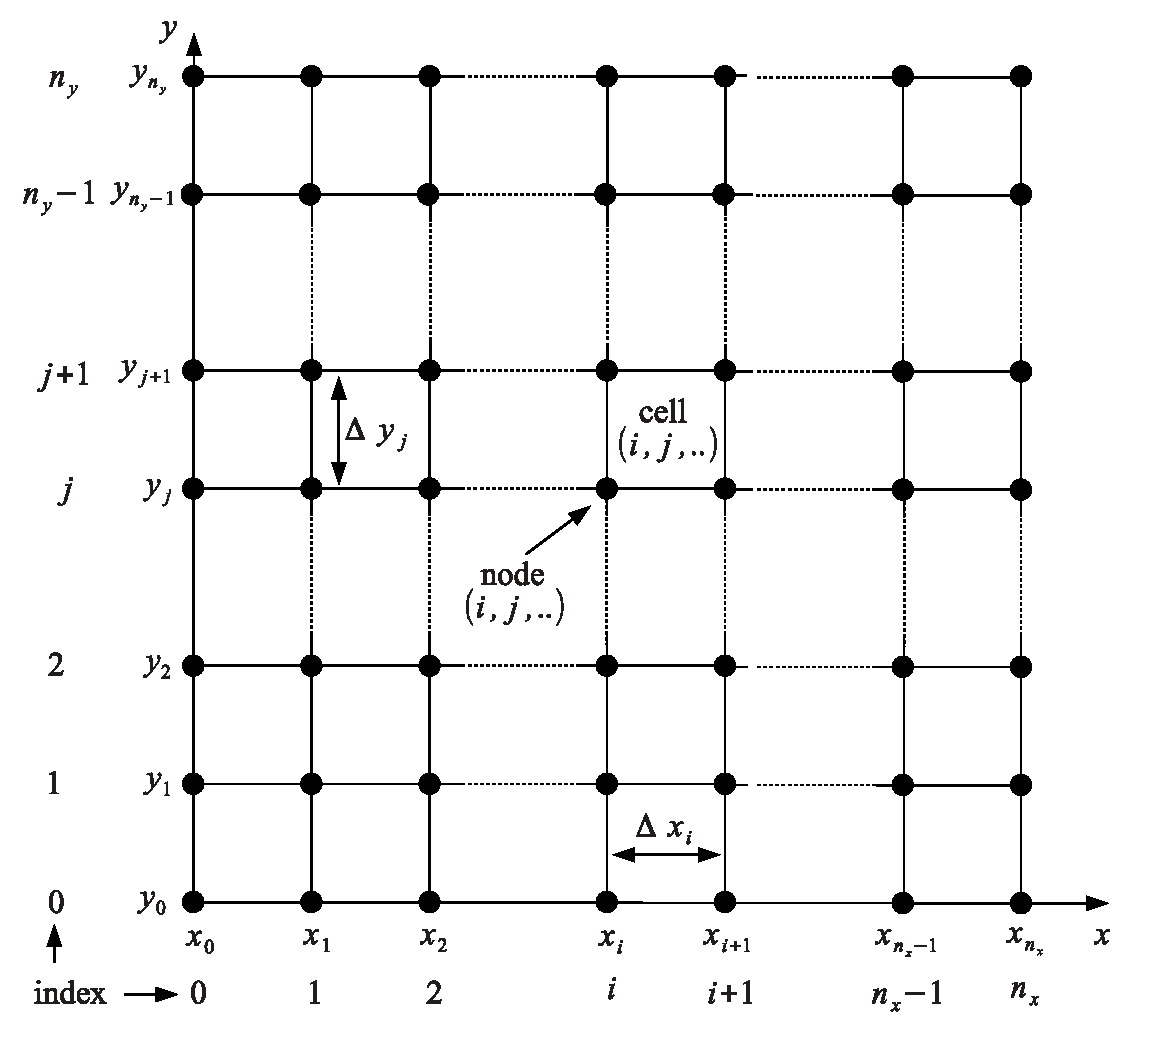
\includegraphics[width=12cm]{figures/meshdefn}}
\caption{\label{fg:meshdefn} Mesh lines and cells in the $x$ and $y$ directions.}
\end{figure}

The structured mesh used by Vulture is defined by a set of mesh lines $x_i$, $y_j$ and $z_k$ in the $x$, $y$ 
and $z$ directions
\begin{eqnarray}
&\{ x_i;& i = 0 \ldots N_x - 1 \} \nonumber \\
&\{ y_j;& j = 0 \ldots N_y - 1 \} \\
&\{ z_k;& k = 0 \ldots N_z - 1 \},  \nonumber
\end{eqnarray}
where $N_x$, $N_y$ and $N_z$ are the number of mesh lines in each direction (see Figure~\ref{fg:meshdefn}). The mesh lines are
labelled by the indices $i$, $j$ and $k$. The intersection points of the mesh lines define a 
set of nodes labelled by the indices of the intersecting mesh lines, $(i,j,k)$, and the lines (edges) 
between the nodes partition the volume of the mesh into $(N_x-1) \times (N_y-1) \times (N_z-1) \equiv n_x \times n_y \times n_z$ cuboid cells.
These cell form the primary grid or lattice. The cells are labelled by the indices of the mesh lines on the low coordinate side of the 
cell, so we have cells number indices $0,\ldots,n_x-1$ etc. The cell sizes are given by
\begin{eqnarray}
& \{\Delta x_i = x_{i+1} - x_i ; i = 0 \ldots n_x-1 \} \nonumber \\
& \{\Delta y_j = y_{j+1} - y_j ; j = 0 \ldots n_y-1 \}.  \\
& \{\Delta z_k = z_{k+1} - z_k ; k = 0 \ldots n_z-1 \} \nonumber
\end{eqnarray}
The electric field is sampled at the centres of the primary grid edges at times $t=n \Delta t\,\,(n=0,\ldots,N_\mathrm{s}-1)$:
$E^{n}_x(i+\half,j,k)$, $E^{n}_y(i,j+\half,k)$ and $E^{n}_z(i,j,k+\half)$.
The cell centres are at the coordinates
\begin{eqnarray}
\{ &x_{i+\half} = x_i + \Delta x_i / 2;& i = 0 \ldots N_x-2 \} \nonumber \\
\{ &y_{j+\half} = y_j + \Delta y_j / 2;& j = 0 \ldots N_y-2 \} \nonumber \\
\{ &z_{k+\half} = z_k + \Delta z_k / 2;& k = 0 \ldots N_z-2 \}.
\end{eqnarray}
The {\em dual} or {\em secondary lattice} is then defined to be the grid whose
vertices are the primary lattice centres,
\begin{eqnarray}
\{ &x_{i+\half};& i = 0 \ldots N_x-2 \} \nonumber \\
\{ &y_{j+\half};& j = 0 \ldots N_y-2 \} \nonumber \\
\{ &z_{k+\half};& k = 0 \ldots N_z-2 \},
\end{eqnarray}
and the edge lengths of the dual lattice are
\begin{eqnarray}
\{ &\tilde{\Delta} x_i = x_{i+\half} - x_{i-\half}  = (\Delta x_i + \Delta x_{i-1})/2;& i = 1 \ldots N_x-2 \} \nonumber \\
\{ &\tilde{\Delta} y_j = y_{j+\half} - y_{j-\half}  = (\Delta y_j + \Delta y_{j-1})/2;& j = 1 \ldots N_y-2 \} \nonumber \\
\{ &\tilde{\Delta} z_k = z_{k+\half} - z_{k-\half}  = (\Delta z_k + \Delta z_{k-1})/2;& k = 1 \ldots N_z-2 \}.
\end{eqnarray}
The magnetic field is sampled at the centres of the secondary grid edges at times $t=(n+\half)\Delta t\,\,(n=0,\ldots,N_\mathrm{s}-1)$:
$H^{n+\half}_x(i,j+\half,k+\half)$, $H^{n+\half}_y(i+\half,j,k+\half)$ and $H^{n+\half}_z(i+\half,j+\half,k)$. The locations of the
electric and magnetic fields in the primary are is shown in Figure~\ref{fg:yeecell}.

\begin{figure}[t]
\centerline{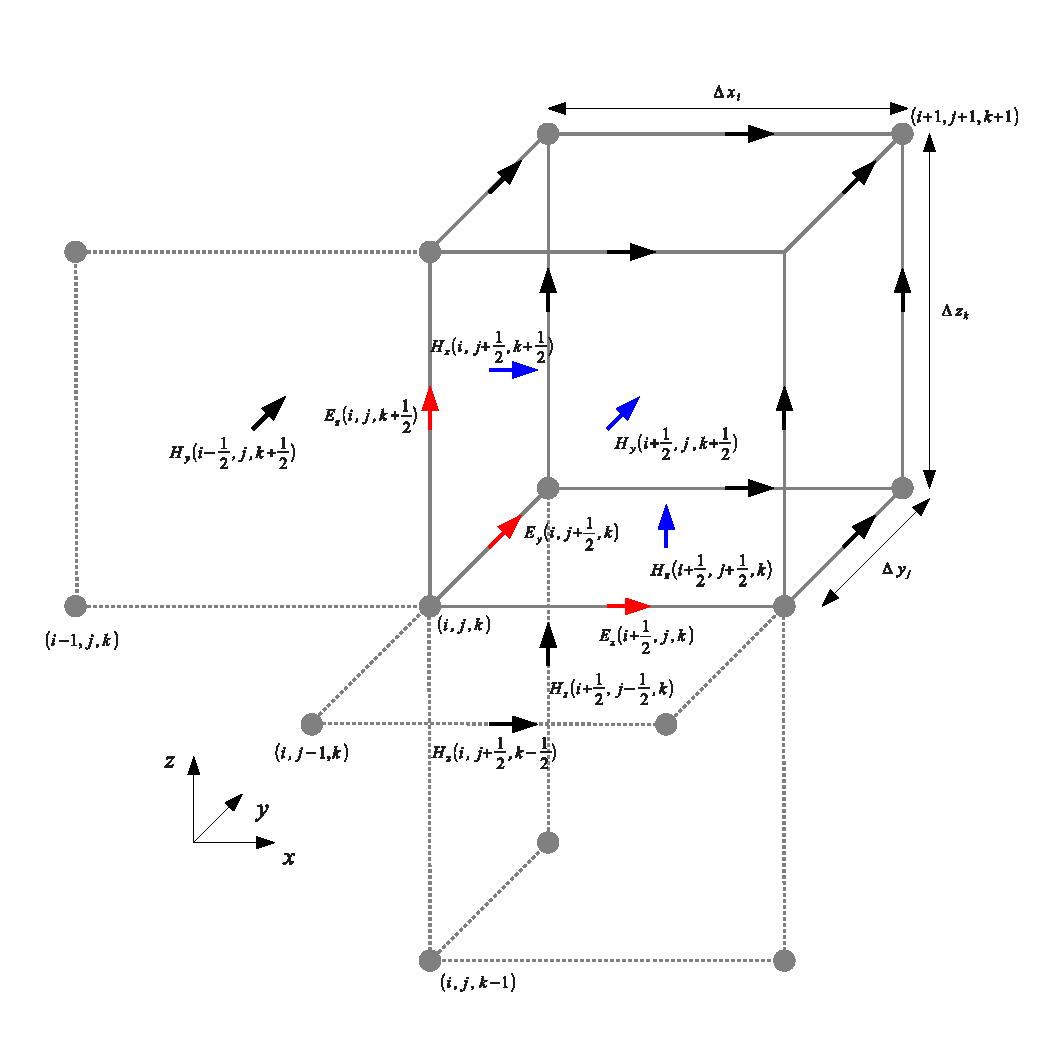
\includegraphics[width=0.9\linewidth]{figures/yeecell}}
\caption{\label{fg:yeecell}Location of the field sampling points in the primary FDTD grid.}
\end{figure}

In the mesh file the overall mesh extents are specified in Section 1
using the numbers of cells $(n_x,n_y,n_z)$ with the \texttt{DM} directive:
\begin{verbatim}
DM <i: nx> <i: ny> <i: nz> 
\end{verbatim}
The mesh sizes are defined in Section 3 of the mesh file.
Uniform meshes are defined using an \texttt{MS} directive to specify the constant edge lengths 
\texttt{<r:~delx>} ($\Delta x$), \texttt{<r:~dely>} ($\Delta y$) and \texttt{<r:~delz>}
($\Delta z$) in the three coordinate directions:
\begin{verbatim}
MS <r: delx> [ <r: dely> <r: delz> ] ]
\end{verbatim} 
The edge lengths are specified in metres. If \texttt{<r:~dely>} and/or \texttt{<r:~delz>} are missing the edge 
length from the previous coordinate direction is used. A uniform cubic mesh can therefore be defined using
\begin{verbatim}
MS <r: del>
\end{verbatim}
in which case $\Delta x_i=\Delta y_j=\Delta z_k=\Delta\,(\forall i,j,k)$. The physical coordinates of the mesh lines are defined automatically 
for a uniform mesh starting at $x_0=y_0=z_0=0$\,m. For non-uniform meshes the \texttt{MS} directive is replaced by \texttt{XL},  \texttt{YL} 
and \texttt{ZL} directives which explicitly give the physical coordinates of all the mesh lines in metres:
\begin{verbatim}
XL 
<r: x[0]>
.....
<r: x[nx]>
YL 
<r: y[0]> 
.....
<r: y[ny]>
ZL
<r: z[0]> 
.....
<r: z[nz]>
\end{verbatim}

% --
\subsection{Bounding boxes}
% --
Objects on the mesh are specified by a bounding box selector which references a physical model or other
entity such as a source or observer. An inclusive bounding box consists of a set of six integer mesh line indices 
$[i_\mathrm{lo},i_\mathrm{hi},j_\mathrm{lo},j_\mathrm{hi},k_\mathrm{lo},k_\mathrm{hi}]$ that selects all the
compatible mesh elements within and on its surface:
\begin{eqnarray}
[i_\mathrm{lo},i_\mathrm{hi},j_\mathrm{lo},j_\mathrm{hi},k_\mathrm{lo},k_\mathrm{hi}] =
\{ i: i_\mathrm{lo} \le i \le i_\mathrm{hi},
   j: j_\mathrm{lo} \le j \le j_\mathrm{hi},
   k: k_\mathrm{lo} \le k \le k_\mathrm{hi}\}. \nonumber
\end{eqnarray}
Such bounding boxes are able to select single nodes, edges, faces, surfaces and volumes on the mesh.
Bounding boxes are required to be {\em normal} in the sense defined by
\begin{eqnarray}
i_\mathrm{lo} \le i_\mathrm{hi} \nonumber \\
j_\mathrm{lo} \le j_\mathrm{hi} \nonumber \\  
k_\mathrm{lo} \le k_\mathrm{hi},
\label{eq:normalbbox}
\end{eqnarray}
and use the mesh line numbers from $(0,0,0)$ to $(n_x,n_y,n_z)$.
Some examples are:
\begin{verbatim}
2 2 3 3 4 4  # A node at (2,3,4).
2 2 3 3 4 5  # A z-directed edge.
2 2 3 3 4 7  # A z-directed line 3 edges long.
2 2 1 2 1 2  # An x-normal face.
2 2 1 5 1 5  # An x-normal 4x4 face surface.
2 3 3 4 4 5  # A single cell.
2 4 3 5 4 6  # A 2x2x2 cell volume.
\end{verbatim}

% --
\subsection{Simulation time-step control: \texttt{NT}, \texttt{CN}}
% --

The number of time-step iterations to be performed, $N_\mathrm{s}$, is specified by the
\texttt{<i:~numSteps>} parameter in the \texttt{NT} directive:
\begin{verbatim}
NT <i: numSteps>
\end{verbatim}
The FDTD simulation will run for $N_\mathrm{s}$ iterations $n=0,\ldots,N_\mathrm{s}-1$ 
corresponding to times $t=0,\ldots,(N_\mathrm{s}-1)\Delta t$. The time-step is determined
automatically from the mesh-lines using
\begin{eqnarray}
\Delta t = C_N \frac{1}{c_0 \sqrt{ 
\left(\frac{1}{\Delta x_\mathrm{min}}\right)^2 
+\left(\frac{1}{\Delta y_\mathrm{min}}\right)^2
+\left(\frac{1}{\Delta z_\mathrm{min}}\right)^2
} }
\label{eq:ttimestep}
\end{eqnarray}
where $\Delta x_\mathrm{min} = \min_i [ \Delta x_i ,\tilde{\Delta}x_i ]$ etc. are the edge lengths of the
smallest cell in the mesh. Thus the cell with the largest value of $1/(\Delta x_\mathrm{min})^2 
+1/(\Delta y_\mathrm{min})^2+1/(\Delta z_\mathrm{min})^2$ in the mesh determines the time-step. Here the 
Courant-Fredrichs-Lewy Number (CFLN), $C_N$, must be in the range zero to one, $0<C_N\le1$, for the simulation to be stable. By 
default $C_N=\sqrt{3}/2$, in which case on a cubic mesh of edge length $\Delta$ the time-step becomes
\begin{eqnarray}
\Delta t = \frac{\Delta}{2 c_0}
\label{eq:ttimestep2}
\end{eqnarray}
and wavefronts propagating in free-space normal to mesh faces advance by one cell in two time-steps.

The CFLN number can changed using the \texttt{CN} directive:
\begin{verbatim}
CN <r: courantNumber>
\end{verbatim}
Dispersion in the FDTD grid becomes greater as the CFLN is reduced. However, as the CFLN
approaches unity the algorithm has more chance of becoming unstable, depending on which features of the code
are being used.

%
% ----------------------------------------------------------------------- 
%
\section{Physical models}
\label{sc:phymod}
%
% ----------------------------------------------------------------------- 
%

% --
\subsection{Physical models and bounding boxes as selectors}
% --

Physical models for volumetric, surface and line type materials are defined separately 
using \texttt{MT}, \texttt{BT} and \texttt{WT} directives respectively:
\begin{verbatim}
MT <t: name> <t: type> <param1> ... <paramN>
BT <t: name> <t: type> <param1> ... <paramN>
WT <t: name> <t: type> <param1> ... <paramN>
\end{verbatim}
The parameters for these directives are generally independent of the mesh and specific 
to the physical model. The name-spaces of the tags for the voulme, surface and wire
material types are distinct. 

Three corresponding types of selector are defined for physical models on the mesh using
\texttt{MB}, \texttt{TB} and \texttt{TW} directives:
\begin{verbatim}
MB <i: ilo> <i: ihi> <i: jlo> <i: jhi> <i: klo> <i: khi> <t: name> [<param1> ... <paramN>]
TB <i: ilo> <i: ihi> <i: jlo> <i: jhi> <i: klo> <i: khi> <t: name> [<param1> ... <paramN>]
TW <i: ilo> <i: ihi> <i: jlo> <i: jhi> <i: klo> <i: khi> <t: name> [<param1> ... <paramN>]
\end{verbatim}
These select volumes (blocks), surfaces (boundaries) and lines (wires) respectively. These selectors are used to
define the mesh elements on which the physical models referenced by their tags are to be applied.
The parameters are used to define how the model is applied within the bounding box. 

Irrespective of the order in which the physical model directives are declared in Section 2 
of the mesh file they are applied to the computational grid in the following order:
\begin{enumerate}
 \item All \texttt{MB}s in the order found in the mesh.
 \item All \texttt{TB}s in the order found in the mesh.
 \item All \texttt{TW}s in the order found in the mesh.
 \item All \texttt{EX}s in the order found in the mesh.
 \item All \texttt{PW}s in the order found in the mesh.
\end{enumerate}
As will be detailed below \texttt{MB}, \texttt{TB} and \texttt{TW} objects of type \texttt{PEC}, 
\texttt{FREE\_SPACE} and \texttt{SIMPLE} will over-write each other without side effects. Other types 
(e.g SIBCs and dispersive materials) will {\it not} overwrite and will probably generate indeterminate results. 

% --
\subsection{Volumetric materials: \texttt{MT}, \texttt{MB}}
% --

Volumetric material model types are defined using the \texttt{MT} directive which has
the general form:
\begin{verbatim}
MT <t: name> <t: type> <param1> ... <paramN>
\end{verbatim}
Here \texttt{<t:~name>} is the name tag for the material type being defined and must be unique 
amongst all other \texttt{MT} directives. The valid material types, \texttt{<t:~type>}, and 
their parameters are:
\begin{verbatim}
MT <t: name> SIMPLE [ <r: eps_r> [ <r: sigma> [ <r: mu_r> ] ] ]
MT <t: name> FREE_SPACE
MT <t: name> PEC
MT <t: name> DEBYE <r: eps_Inf> <r: sigma> <r: mu_r> <r: res_1> <r: pole_1> \
   [ <r: res_2> <r: pole_2> [ <r: res_3> <r: pole_3> ] ] 
MT <t: name> DEBYE <s: fileName>
\end{verbatim}
The material type tags \texttt{PEC} and \texttt{FREE\_SPACE} are predefined for \texttt{PEC} 
and \texttt{FREE\_SPACE} materials respectively and cannot be overridden, i.e. the directives 
\begin{verbatim}
MT PEC PEC
MT FREE_SPACE FREE_SPACE
\end{verbatim}
have effectively already been applied internally by the solver. 

A material type identified by tag \texttt{<t:~name>} is applied to a volume on the mesh using 
the \texttt{MB} directive:
\begin{verbatim}
MB <i: ilo> <i: ihi> <i: jlo> <i: jhi> <i: klo> <i: khi> <t: name>  [ <t: mask> ]
\end{verbatim}
The bounding box {\em must} define a volume (not a surface, line, edge or node). Volumetric materials 
are the first physical models applied to computational grid with each \texttt{MB} directive applied 
in the order it appears in the mesh file. Materials of type \texttt{SIMPLE}, \texttt{FREE\_SPACE} 
and \texttt{PEC} will overwrite each other without adverse side effects. Other materials types
should not be applied ``on top of each other''. If compilation option {USE\_AVERAGED\_MEDIA=OFF}
(see below) then the optional parameter \texttt{<t:~mask>} can be used
to determine if each external surface of the block is included in the material. The parameter is a
string of six binary digits 0/1 with no spaces between them indicating whether (1) or not (0) the 
surfaces \texttt{XLO}, \texttt{XHI}, \texttt{YLO}, \texttt{YHI}, \texttt{ZLO}, \texttt{ZHI} respectively
of the block are within the material. The default is to include all surfaces, i.e. \texttt{111111}. The string
\texttt{111011} would indicate that all surfaces except \texttt{YHI} should be included.

Depending on the value of the compilation option \texttt{USE\_AVERAGED\_MEDIA}, volumetric materials 
are applied  to the grid in one of two ways:
\begin{itemize}
 \item \texttt{USE\_AVERAGED\_MEDIA=OFF}: The simple material parameters are applied directly to
 all the edges encompassed by the bounding box. This method does not accurately represent the location of 
 interfaces between different media. \texttt{SIMPLE} material types will overwrite when the bounding boxes
 overlap. Overlapping of \texttt{DEBYE} material types is ill-defined and the \texttt{<t:~mask>} option of 
 the \texttt{MB} directive should be used to align such material boundaries precisely {\em without} overlap.
 \item \texttt{USE\_AVERAGED\_MEDIA=ON}: The material parameters are first associated with the entire volume of 
 each cell in  the bounding box, ignoring any \texttt{<t:~mask>} parameters in \texttt{MB} directives. After 
 all the \texttt{MB} directives have been processed the parameters are then 
 averaged across the boundaries of different materials to give a more accurate model for material interfaces
 at the location of the mesh faces (i.e the actual location of the bounding box surfaces). {\em This option does not
 yet correctly support averaging of} \texttt{DEBYE} {\em type media.} For Debye media the high frequency 
 permittivity and (ionic) conductivity terms are averaged, however, the polarisation currents due to the 
 relaxtion terms are not. The polarisation currents are applied directly, as for the case \texttt{USE\_AVERAGED\_MEDIA=OFF},
 respecting any \texttt{<t:~mask>} parameters. Depending on the material parameters and simulation
 geometry this may or may not produce an accurrate model. 
\end{itemize}

\subsubsection{\texttt{SIMPLE} non-dispersive material type}

\begin{verbatim}
MT <t: name> SIMPLE [ <r: eps_r> [ <r: sigma> [ <r: mu_r> ] ] ]
\end{verbatim}

\begin{table}[ht]
\begin{center}
\begin{tabular}{|l|l|c|c|c|}
\hline
Parameter             &Quantity                &Symbol                &Units    &Default  \\  
\hline
\texttt{<r:~eps\_r>}  &Relative permittivity   &$\epsilon_\mathrm{r}$ &-        &1.0      \\
\texttt{<r:~sigma}    &Electrical conductivity &$\sigma$              &S/m      &0.0      \\
\texttt{<r:~mu\_r>}   &Relative permeability   &$\mu_\mathrm{r}$      &-        &1.0      \\ 
\hline
\end{tabular}
\caption{\label{tb:mbsimple}\texttt{SIMPLE} material model parameters.}
\end{center}
\end{table}

The simple material model type, \texttt{SIMPLE}, defines frequency independent isotropic media that
are characterised by a relative permittivity, $\epsilon_\mathrm{r}$, electrical conductivity,
$\sigma$, and a relative permeability, $\mu_\mathrm{r}$. The parameters for this type are defined 
in Table~\ref{tb:mbsimple}.

An example of a simple material model type and its application on a mesh is:
\begin{verbatim}
MT copper SIMPLE 1.0 3.7e7 1.0
MB 10 20 10 20 10 20 copper
\end{verbatim}
This would set the volume enclosed by the bounding box $[10,20,10,20,10,20]$ to have 
the simple material parameters of copper: $\epsilon_\mathrm{r}=1$, $\sigma=37$\,MS/m and 
$\mu_\mathrm{r}=1$.

\subsubsection{\texttt{FREE\_SPACE} material type}

\begin{verbatim}
MT <t: name> FREE_SPACE
\end{verbatim}

The free-space material type, \texttt{FREE\_SPACE}, is a pseudonym for \texttt{SIMPLE 1.0 0.0 1.0}
so the above is equivalent to
\begin{verbatim}
MT <t: name> SIMPLE 1.0 0.0 1.0
\end{verbatim}

\subsubsection{\texttt{PEC} material type}

\begin{verbatim}
MT <t: name> PEC
\end{verbatim}

The PEC material type, \texttt{PEC}, simulates a perfect electric conductor 
in volumes to which it is applied by setting the FDTD update coefficients to 
$\alpha=-1.0$ and $\beta=0.0$ (see the Code Implementation Manual for details~\cite{vultimp}). 
This method is more robust than using a high conductivity to represent a PEC material as in
\begin{verbatim}
MT POORPEC SIMPLE 1.0 1e5
\end{verbatim}
but it behaves in the same way with regard to overwriting of overlapping bounding boxes 
and the averaging of neighbouring materials discussed above.

\subsubsection{\texttt{DEBYE} electrically dispersive material type}

\begin{verbatim}
MT <t: name> DEBYE <r: eps_Inf> <r: sigma> <r: mu_r> <r: res_1> <r: pole_1> \
   [ <r: res_2> <r: pole_2> [ <r: res_3> <r: pole_3> ] ] 
MT <t: name> DEBYE <s: fileName>
\end{verbatim}

The \texttt{DEBYE} material type defines a frequency dependent electrically dispersive material
characterised by a multi-pole generalised Debye dispersion relationship. The dispersion relationship 
for an $N_m$-pole relaxation is given by
\begin{eqnarray}
\hat{\epsilon}_r(\omega) = \epsilon_\infty - \frac{\jmath \sigma}{\omega \epsilon_0}
+\sum_{k=1}^{N_m} \left\{ \frac{r_k}{\jmath\omega - p_k} + \frac{r^*_k}{\jmath\omega - p^*_k} \right\},
\end{eqnarray}
where $\epsilon_{\infty}$ is the relative permittivity in the high frequency limit, 
$\sigma$ is an ionic conductivity term, $r_k$ is the residue of the $k$-th pole and $p_k$ is the 
$k$-th pole. Using this formulation the poles are enforced to occur in complex conjugate pairs.
Such parameterisations can, for example, be obtained using a vector fitting algorithm~\cite{Gustavsen1999}.
A standard Debye relaxation is a special case with a real residue and pole given by
\begin{eqnarray}
p_k &=& -\frac{1}{\tau_k} \\
r_k &=& \frac{\Delta \epsilon_k}{2 \tau_k} \\
 \left\{ \frac{r_k}{\jmath\omega - p_k} + \frac{r^*_k}{\jmath\omega - p^*_k} \right\}
&\rightarrow&
\frac{\Delta \epsilon_k}{1+\jmath\omega\tau_k}, 
\end{eqnarray}
where $\Delta \epsilon_k=\epsilon_{\mathrm{static};k}-\epsilon_{\infty;k}$ is the decrement caused by the $k$-th 
pole and $\tau_k$ is the relaxtion time of the pole. Here $\epsilon_{\mathrm{s};k}$ is the static, low frequency permittivity associated 
with the $k$-th relaxation.
A second-order Lorentz dispersion is given by
\begin{eqnarray}
p_k &=& -\delta_k -\jmath \sqrt{ \omega^2_k - \delta^2_k } \\
r_k &=& \frac{\jmath \Delta \epsilon_k \omega^2_k}{2 \sqrt{ \omega^2_k - \delta^2_k }} \\
 \left\{ \frac{r_k}{\jmath\omega - p_k} + \frac{r^*_k}{\jmath\omega - p^*_k} \right\}
&\rightarrow&
\frac{\Delta \epsilon_k \omega^2_k}{\omega^2_k+2\jmath\omega\delta_k-\omega^2}.
\end{eqnarray}
The parameters are summarised in Table~\ref{tb:mbdebye}, where the poles and residues are taken to be real. 
For a stable causal model it is required that $\epsilon_{\infty} \ge 1$ and $\Re(p_k) \le 0$.
For up to three real poles the Debye parameters can be specified directly in the mesh file. For complex
poles and higher orders the parameters must be specified in an external ASCII file, referenced by the file 
name parameter \texttt{<s:~fileName>}, that has the format given in Table~\ref{tb:mbdebext}. {\em Note that
only one residue/pole of each complex conjugate pair should be entered - the other is included implicitly!}

\begin{table}[ht]
\begin{center}
\begin{tabular}{|l|l|c|c|c|}
\hline
Parameter              &Quantity                             &Symbol              &Units         &Default  \\  
\hline
\texttt{<r:~eps\_Inf>} &High frequency relative permittivity &$\epsilon_\infty$   &-             &1.0       \\
\texttt{<r:~sigma>}    &(Ionic) electrical conductivity      &$\sigma$            &S/m           &0.0       \\
\texttt{<r:~res\_k>}   &Residue                              &$r_k$               &rad\,s$^{-1}$ &none      \\ 
\texttt{<r:~pole\_k>}  &Pole                                 &$p_k$               &rad\,s$^{-1}$ &none      \\
\hline
\end{tabular}
\caption{\label{tb:mbdebye}\texttt{DEBYE} material model parameters.}
\end{center}
\end{table}

\begin{table}[ht]
\begin{center}
\begin{Verbatim}[frame=single]
<i: N_m> <r: eps_inf> <r: sigma> <r: mu_r>
Re[<r: res_1>]   Im[<r: res_1>]   Re[<r: pole_1>]   Im[<r: pole_1>]
...              ...              ...               ...
Re[<r: res_N>]   Im[<r: res_N>]   Re[<r: pole_N>]   Im[<r: pole_N>]
\end{Verbatim}
\vspace{-3mm}
\caption{\label{tb:mbdebext}External file format for the \texttt{DEBYE} material type. Comment and blank lines are not allowed.}
\end{center}
\end{table}

% --
\subsection{Internal and external surface materials, \texttt{BT}, \texttt{TB}}
% --

Surface material model types - called boundary types - are defined using the \texttt{BT} directive 
which has the general form:
\begin{verbatim}
BT <t: name> <t: type> <param1> ... <paramN>
\end{verbatim}
Here \texttt{<t:~name>} is the name tag for the boundary type being defined and must be unique 
amongst all other \texttt{BT} directives. The valid boundary types, \texttt{<t:~type>}, and 
their parameters are:
\begin{verbatim}
BT <t: name> FREE_SPACE
BT <t: name> PEC
BT <t: name> PMC
BT <t: name> PERIODIC
BT <t: name> MUR
BT <t: name> PML <i: nlayer> <i: order> <rl: n_eff> <rl: refcoeff> <rl: kmax>
BT <t: name> SIBC  <r: S11_TM> <r: S12_TM> <r: S21_TM> <r: S22_TM> \
                 [ <r: S11_TE> <r: S12_TE> <r: S21_TE> <r: S22_TE> ]
BT <t: name> SIBC  <s: fileName>
\end{verbatim}
The boundary type tags \texttt{PEC}, \texttt{PMC} and \texttt{FREE\_SPACE} are predefined for \texttt{PEC}, \texttt{PMC} 
and \texttt{FREE\_SPACE} boundary types respectively and cannot be overridden, i.e. the directives 
\begin{verbatim}
BT PEC PEC
BT PMC PMC
BT FREE_SPACE FREE_SPACE
\end{verbatim}
are effectively applied internally by the solver. The valid usage of the
different boundary types on internal and external surfaces of the mesh is summarised in Table~\ref{tb:bt}.

\begin{table}[ht]
\begin{center}
\begin{tabular}{|l|c|c|c|}\hline
Boundary type         &Internal surface      &External surface  &Over-write \\  \hline
\texttt{FREE\_SPACE}  &Yes                   &No                &Yes        \\
\texttt{PEC}          &Yes                   &Yes               &Yes        \\
\texttt{PMC}          &No                    &Yes               &No         \\
\texttt{PERIODIC}     &No                    &Yes               &n/a        \\
\texttt{MUR}          &No                    &Yes               &n/a        \\
\texttt{PML}          &No                    &Yes               &n/a        \\
\texttt{SIBC}         &Yes                   &No                &Limited    \\ \hline
\end{tabular}
\caption{\label{tb:bt} Valid usage of different boundary types.}
\end{center}
\end{table}

A boundary type identified by tag \texttt{<t:~name>} is applied to a surface on the mesh using 
the \texttt{TB} directive:
\begin{verbatim}
TB <i: ilo> <i: ihi> <i: jlo> <i: jhi> <i: klo> <i: khi> <t: name> \
   [ <i: orient> [ <r: angle> ] ]
\end{verbatim}
The bounding box must define a surface (not a volume, line, edge or node). The parameters 
\texttt{<i:~orient>} and \texttt{<r:~angle>} are used to orientate and align asymmetric and
anisotropic boundary type materials on the computational grid as discussed below.

Boundary type materials are the second type of physical model applied to computational grid, after 
the volumetric materials, with each \texttt{TB} directive applied in the order it appears in 
the mesh file. Boundaries of type \texttt{FREE\_SPACE} and \texttt{PEC} will overwrite each 
other without adverse side effects. SIBC boundaries can be applied (once) on top of PEC boundaries.
Other boundary types should not be applied ``on top of each other''.

\subsubsection{External surfaces}

Boundary type tags for the boundaries forming each external face of the mesh are predefined by the solver
and associated with those surfaces. This is equivalent to the directives
\begin{verbatim}
TB  0  0  0 ny  0 nz XLO
TB nx nx  0  0  0 nz XHI
TB  0 nx  0  0  0 nz YLO
TB  0 ny ny ny  0 nz YHI
TB  0 nx  0 ny  0  0 ZLO
TB  0 nx  0 ny nz nz ZHI
\end{verbatim}
having been applied, where \texttt{nx, ny, nz} are the mesh extents. So, for example, \texttt{XLO} is a tag 
for the boundary type of the $x$-normal external face of the mesh on the lower $x$ side of the mesh. 
These tags can used to define the boundary types on the external mesh surfaces using \texttt{BT} directives,
somewhat in reverse to the way they are used for all other internal surfaces. By default all the external 
surfaces are PML absorbing boundary types with default parameters, i.e. the directives
\begin{verbatim}
TB XLO PML
TB XHI PML
TB YLO PML
TB YHI PML
TB ZLO PML
TB ZHI PML
\end{verbatim}
are applied by default. Only boundary types \texttt{PEC}, \texttt{PMC}, \texttt{PERIODIC}, \texttt{MUR} and \texttt{PML} are
valid on external surfaces.

\subsubsection{\texttt{PEC} boundary type}

\begin{verbatim}
BT <t: name> PEC
\end{verbatim}

The \texttt{PEC} boundary type enforces zero tangential electric field on a surface
by setting the FDTD update coefficients to $\alpha=-1.0$ and $\beta=0.0$
(see the Code Implementation Manual for details~\cite{vultimp}).

The following example defines a closed PEC box: 
\begin{verbatim}
BT walls PEC 
TB 10 10 10 20 10 20 walls
TB 20 20 10 20 10 20 walls
TB 10 20 10 20 10 10 walls
TB 10 20 10 20 20 20 walls
TB 10 20 10 10 10 20 walls
TB 10 20 20 20 10 20 walls
\end{verbatim}

\subsubsection{\texttt{PMC} boundary type}

\begin{verbatim}
BT <t: name> PMC
\end{verbatim}

The \texttt{PMC} boundary type enforces a PMC boundary condition on an external
surface using a field mirroring algorithm with ghost fields ``outside'' the computational
grid. In this way the PMC is located on the primary grid faces, the same as \texttt{PEC}
boundary types on external surfaces.

For example an infinite parallel plate waveguide with metal plates on the lower and upper
$z$-normal external surfaces can be defined using:
\begin{verbatim}
BT XLO PMC
BT XHI PMC
BT YLO PEC
BT YHI PEC
BT ZLO PML
BT ZHI PML
\end{verbatim}

PMC boundary types can also be used to create symmetry planes, for example:
\begin{verbatim}
BT XLO PML
BT XHI PML
BT YLO PMC
BT YHI PML
BT ZLO PML
BT ZHI PML
\end{verbatim}
would create a symmetry plane in the \texttt{YLO} mesh surface.

\subsubsection{\texttt{PERIODIC} boundary type}

\begin{verbatim}
BT <t: name> PERIODIC
\end{verbatim}

The \texttt{PERIODIC} boundary type enforces a periodic boundary condition between pairs of external
surfaces \texttt{XLO/XHI}, \texttt{YLO/YHI} and \texttt{ZLO/ZHI}, using a field copying 
algorithm with ghost fields ``outside'' the computational grid. The boundary condition is located on 
the primary grid faces, the same as other boundary types on external surfaces. Opposite pairs of
external faces {\em must} both be defined with the \texttt{PERIODIC} boundary type.

For example an infinite parallel plate waveguide with metal plates on the lower and upper
$z$-normal external surfaces can be defined using:
\begin{verbatim}
BT XLO PERIODIC
BT XHI PERIODIC
BT YLO PEC
BT YHI PEC
BT ZLO PML
BT ZHI PML
\end{verbatim}

\subsubsection{\texttt{FREE\_SPACE} boundary type}

\begin{verbatim}
BT <t: name> FREE_SPACE
\end{verbatim}

The \texttt{FREE\_SPACE} boundary type imposes free-space material parameters on a
surface. The main use of this boundary type is to ``punch'' holes through
internal \texttt{PEC} type surfaces to create apertures. For example:
\begin{verbatim}
BT walls PEC 
BT aperture FREE_SPACE
# First make a closed metal box.
TB 10 10 10 20 10 20 walls
TB 20 20 10 20 10 20 walls
TB 10 20 10 20 10 10 walls
TB 10 20 10 20 20 20 walls
TB 10 20 10 10 10 20 walls
TB 10 20 20 20 10 20 walls
# Then punch hole in face.
TB 10 10 12 18 12 18 aperture
\end{verbatim}

Note that this does not work for SIBC types surfaces!

\subsubsection{\texttt{MUR} boundary type}

\begin{verbatim}
BT <t: name> MUR
\end{verbatim}

The \texttt{MUR} boundary type specifies a first order Mur analytic ABC for external surfaces. It is compatible
with \texttt{PEC} and \texttt{PMC} boundary types on neighbouring surfaces. It gives a normal incidence 
free-space reflection coefficient of approximately -20\,dB providing sufficient space is left between
it and scattering objects on the grid (about half a wavelength).

\subsubsection{\texttt{PML} boundary type}

\begin{verbatim}
BT <t: name> PML <i: nlayer> <i: order> <r: n_eff> <r: refcoeff> <r: kmax>
\end{verbatim}

The \texttt{PML} boundary type specifies a perfectly matched layer (PML) ABC for external surfaces.
This is a more advanced ABC than the Mur with much better performance, albeit at a significantly 
higher computational cost. The PML boundary
type adds a number of layers, $n_\mathrm{layer}$, of fictitious matched absorbing material to the 
external face of the mesh. Adding more layers improves the performance, i.e. reduces the 
reflections from the face, but increases the memory requirements and run-time of the simulation.  
Vulture implements a Uniaxial PML (UPML) with complex stretching factor~\cite{vultimp}
\begin{eqnarray}
s(x) = \kappa(x) + \frac{\sigma (x)}{\ri \omega \epsilon_0}
\end{eqnarray}
and polynomial grading profiles
\begin{eqnarray}
\sigma(x) &=& \sigma^{\mathrm{max}} \left(\frac{x}{d}\right)^m \\
\kappa(x) &=& 1 + (\kappa^{\mathrm{max}}-1) \left( \frac{x}{d} \right)^m.
\end{eqnarray}
Here $x$ is the perpendicular distance into the PML and $d$ is the total thickness of
the PML. The maximum PML conductivity, $\sigma^{\mathrm{max}}$, is related to the magnitude of
the theoretical (continuous space) reflection coefficient, $|R(0)|$ by 
\begin{eqnarray}
\sigma^{\mathrm{max}} = -\frac{m+1}{2 \eta d} \ln \left| R(0) \right|.
\end{eqnarray}
This has an empirically determined optimum value of 
\begin{eqnarray}
\sigma^{\mathrm{opt}} = \frac{4}{\eta \Delta} \frac{m+1}{5} = \frac{4 n_\mathrm{eff}}{\eta_0 \Delta l} \frac{m+1}{5},
\end{eqnarray}
where $\Delta$ is the mesh size of the PML cells in the direction 
perpendicular to the surface and $n_\mathrm{eff}$ is the effective refractive index
of the dominant mode(s) incident on the PML. The PML parameters and their
default values are defined in Table~\ref{tb:tbpml}. 

\begin{table}[ht]
\begin{center}
\begin{tabular}{|l|l|c|c|c|}
\hline
Parameter              &Quantity                   &Symbol                &Units &Default \\  
\hline
\texttt{<i:~nlayer>}   &Number of layers           &$n_\mathrm{layer}$    &-     &6       \\
\texttt{<i:~order>}    &Profile order              &m                     &-     &4       \\
\texttt{<r:~n\_eff>}   &Effective refractive index &$n_\mathrm{eff}$      &-     &1.0     \\
\texttt{<r:~refcoeff>} &Reflection coefficient     &$|R(0)|$              &-     &-1$^*$  \\
\texttt{<r:~kmax>}     &Maximum PML permittivity    &$\kappa_\mathrm{max}$ &-     &1.0     \\ 
\hline
\end{tabular}
\caption{\label{tb:tbpml}\texttt{PML} boundary type model parameters. $^*$ indicates optimal value 
should be chosen automatically}
\end{center}
\end{table}

While the PML has substantially improved performance relative to the Mur ABC it has limitiations:
\begin{itemize}
 \item The reflection coefficient begins to increase at grazing angles of incidence which can be a
 problem on high apsect ratio meshes.
 \item The PMLs performance at transparently terminating evanescent waves is limited. The PML permittivity 
 parameter $\kappa$ is useful for improving the performance in this respect. Typically values of 
 $\kappa$ from 5 to 80 have been found to be useful.
\end{itemize}

The Vulture PML implementation allows inhomogeneous
simple materials to be place in contact with PML boundaries and PEC type internal boundaries
normal to the PML surface can also be placed in contact with the PML. This effectively
simulates the medium touching the PML being extended in the normal direction to infinity. 
The PML is also 
consistent with PEC, PMC and PERIODIC boundary types on neighbouring external surfaces.
Support for electrically dispersive materials is currently only partially implemented.
 
For example, a 10 layer PML with a cubic polynomial profile can de defined using:
\begin{verbatim}
BT ZLO PML 10 3     
\end{verbatim}

\subsubsection{\texttt{SIBC} boundary type}

\begin{verbatim}
BT <t: name> SIBC <s: fileName>
BT <t: name> SIBC  <r: Saa_TM> <r: Sab_TM> <r: Sba_TM> <r: Sbb_TM> \
                 [ <r: Saa_TE> <r: Sab_TE> <r: Sba_TE> <r: Sbb_TE> ]
TB <i: ilo> <i: ihi> <i: jlo> <i: jhi> <i: klo> <i: khi> <t: name> \
   [ <i: orient> [ <r: angle> ] ]
\end{verbatim}

\begin{figure}[ht]
  \begin{center}
    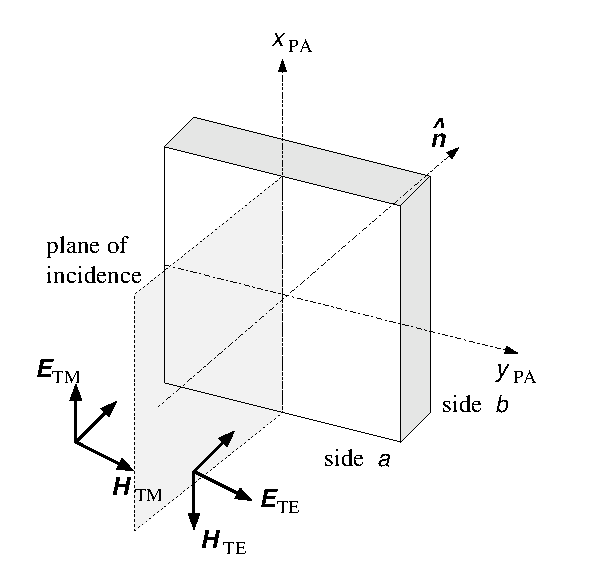
\includegraphics[width=0.40\linewidth]{figures/axesdef}
    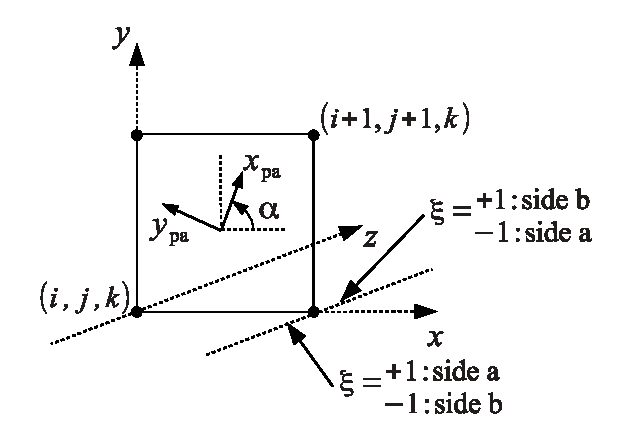
\includegraphics[width=0.49\linewidth]{figures/sibc}
  \end{center}
  \caption{\label{fg:sibc}Definition of SIBC impedance matrix (left) and alignment SIBCs on the mesh for a
  $z$-normal surface(right). The conventions for $x$- and $y$-normal surface are given by cyclic permutation.}
\end{figure}

Note that the SIBC boundary type is a compile time option that is enabled by setting the 
compilation option \texttt{WITH\_SIBC=ON} and may not be available in a particular solver executable.

SIBC boundary types are arbitrary frequency dependent
reflection and transmission boundaries. In general the tangential fields on each 
side of an anisotropic boundary representing a thin material can be resolved into 
transverse electric (TE) and transverse magnetic (TM) waves (see Figure~\ref{fg:sibc}). 
The SIBC model relates these tangential electric and magnetic fields 
using a surface impedance matrix. A natural convention for defining the surface 
impedance matrix is with the TM and TE ports blocked together on either side of the boundary.
In the principal axis system of the material the impedance matrix is block diagonal and
the SIBC can be written
\begin{eqnarray}
\left[
\begin{array}{c}
E^\mathrm{TM}_\mathrm{a}(\omega) \\
E^\mathrm{TM}_\mathrm{b}(\omega) \\
E^\mathrm{TE}_\mathrm{a}(\omega) \\
E^\mathrm{TE}_\mathrm{b}(\omega)
\end{array}
\right]
=
\left[
\begin{array}{cccc}
Z^\mathrm{TM}_{aa}(\omega) &Z^\mathrm{TM}_{ab}(\omega) &0 & 0 \\
Z^\mathrm{TM}_{ba}(\omega) &Z^\mathrm{TM}_{bb}(\omega) &0 & 0 \\
0 & 0 &Z^\mathrm{TE}_{ab}(\omega) &Z^\mathrm{TE}_{aa}(\omega) \\
0 & 0 &Z^\mathrm{TE}_{ba}(\omega) &Z^\mathrm{TE}_{bb}(\omega)
\end{array}
\right]
\left[
\begin{array}{c}
H^\mathrm{TM}_\mathrm{a}(\omega) \\
-H^\mathrm{TM}_\mathrm{b}(\omega) \\
H^\mathrm{TE}_\mathrm{a}(\omega) \\
-H^\mathrm{TE}_\mathrm{b}(\omega)
\end{array}
\right]
\equiv \mZ(\omega) 
\left[
\begin{array}{c}
H^\mathrm{TM}_\mathrm{a}(\omega) \\
-H^\mathrm{TM}_\mathrm{b}(\omega) \\
H^\mathrm{TE}_\mathrm{a}(\omega) \\
-H^\mathrm{TE}_\mathrm{b}(\omega)
\end{array}
\right]
\end{eqnarray}
with two 2-by-2 sub-matrices for the TM and TE polarisations. 
Here ``a'' and ``b'' denote the two sides of the boundary.
For a reciprocal material
\begin{eqnarray}
Z_{ij}(\omega) = Z_{ji}(\omega), 
\end{eqnarray}
while if the material is isotropic
\begin{eqnarray}
Z^\mathrm{TM}_{ij}(\omega) = Z^\mathrm{TE}_{ij}(\omega) \equiv Z_{ij}(\omega).
\end{eqnarray}

The TM and TE polarisations are defined with reference to a local reference system on the 
surface of the material. Aligning this with the global coordinate system of a computational 
grid requires two parameters to be specified for each surface on which the SIBC is applied:
\begin{itemize}
 \item \texttt{<i:~orient>} ($\xi$): A binary orientation flag that indicates which side of 
 the material is on which side of the surface. $\xi=+1$ indicates the ``a'' side of the material is on the lower
 perpendicular coordinate side of the surface while $\xi=-1$ indicates the converse.
 \item \texttt{<r:~angle>} ($\alpha$): The angle between the $x$/$y$/$z$ coordinate axis on the mesh 
 and the $x_\mathrm{pa}$ reference axes on the material for $z$/$x$/$y$-normal surfaces respectively.
\end{itemize}
The conventions are shown in Figure~\ref{fg:sibc} and the SIBC parameters and their default values 
are summarised in Table~\ref{tb:tbsibc}. \texttt{SIBC} boundary types can only be used on internal surfaces.

\begin{table}[ht]
\begin{center}
\begin{tabular}{|l||l|c|c|c|}
\hline
Parameter              &Quantity                       &Symbol   &Units    &Default  \\  
\hline
\texttt{<s:~filename>} &File name                      &n/a      &-        &6        \\
\texttt{<i:~orient>}   &Orientation of sides ($\pm 1$) &$\xi$    &-        &+1       \\
\texttt{<r:~angle>}    &Angle of principal axes        &$\alpha$ &degrees  &0.0      \\ 
\hline
\end{tabular}
\caption{\label{tb:tbsibc}\texttt{SIBC} boundary type model parameters.}
\end{center}
\end{table}

The impedance matrix is related to the scattering matrix of the surface by
\begin{eqnarray}
\mS
=
\left( \mZ - {\mZ}_0 \right)
\left( \mZ + {\mZ}_0 \right)^{-1},
\end{eqnarray}
where
\begin{align}
\mZ_0 &= \mathrm{diag} \left[ \eta_\mathrm{TM}^a , \eta_\mathrm{TE}^b , \eta_\mathrm{TE}^a, \eta_\mathrm{TE}^b \right]
\end{align}
is a diagonal matrix holding the intrinsic impedances of the media on either side of the boundary.
Note that the scattering matrix is specific to the medium surrounding the boundary whereas the impedance
matrix is not. 

The frequency dependent impedance matrix elements are represented by partial fraction 
expansions (PFEs) in the $s$-plane
\begin{eqnarray}
Z_{ij}(s=\jmath \omega)
=
Z^\infty_{ij} + \sum_{k=1}^{N_{ij}}
\frac{r^k_{ij}}{s-p^k_{ij}}\,\,\,\,\,\,(i,j=1,\ldots,M)
\end{eqnarray}
where $Z^\infty_{ij}$ is the high frequency asymptotic response, $N_{ij}$ is 
the order of the $(i,j)$-th element and $r^k_{ij}$ and $p^k_{ij}$ are the $k$-th complex
residues and poles of the $(i,j)$-th element. Typically the order is the same for each element, however, this
does not need to be the case. Frequency independent boundaries are a special case with
$N_{ij}=0\,(\forall i,j)$. 

The PFE representation automatically ensures causality of the SIBC. Stability requires 
that the poles all lie in the left-hand side of the complex plane ($\Re[p^k_{ij}]<0$) and passivity
requires that $\Re[Z_{ij}(\omega)]\ge 0\,\,\forall\omega$. The latter condition can be difficult
to ensure since it applies to {\it all} frequencies, including those far above the frequency
at which the mesh becomes under-sampled. 

The PFEs are specified in an external ASCII format file 
referenced by the \texttt{<s:~filename>} parameter. Denoting $r^k_{ij}$ by 
\texttt{r(i,j,k)}, $p^k_{ij}$ by \texttt{p(i,j,k)} and
$N_{ij}$ by \texttt{N(i,j)} the general format of this PFE input file is
given in Table~\ref{tb:prm}. Vulture currently supports three cases of SIBC
in external files determined by the order of the impedance matrix, $M$:
\begin{itemize}
 \item $M=1$: {\color{red} NOT IMPLEMENTED YET: One-sided (no transmission) isotropic symmetrical material}.
 \item $M=2$: Two-sided isotropic material.
 \item $M=4$: Two-sided anisotropic material.
\end{itemize}
For frequency independent boundaries real valued scattering
parameters
\begin{eqnarray}
\left[
\begin{array}{c}
E^\mathrm{TM-}_\mathrm{a} \\
E^\mathrm{TM-}_\mathrm{b} \\
E^\mathrm{TE-}_\mathrm{a} \\
E^\mathrm{TE-}_\mathrm{b}
\end{array}
\right]
=
\left[
\begin{array}{cccc}
S^\mathrm{TM}_{aa} &S^\mathrm{TM}_{ab} &0 & 0 \\
S^\mathrm{TM}_{ba} &S^\mathrm{TM}_{bb} &0 & 0 \\
0 & 0 &S^\mathrm{TE}_{ab} &S^\mathrm{TE}_{aa} \\
0 & 0 &S^\mathrm{TE}_{ba} &S^\mathrm{TE}_{bb}
\end{array}
\right]
\left[
\begin{array}{c}
E^\mathrm{TM+}_\mathrm{a} \\
E^\mathrm{TM+}_\mathrm{b} \\
E^\mathrm{TE+}_\mathrm{a} \\
E^\mathrm{TE+}_\mathrm{b}
\end{array}
\right]
\equiv \mS
\left[
\begin{array}{c}
E^\mathrm{TM+}_\mathrm{a} \\
E^\mathrm{TM+}_\mathrm{b} \\
E^\mathrm{TE+}_\mathrm{a} \\
E^\mathrm{TE+}_\mathrm{b}
\end{array}
\right]
\end{eqnarray}
can be specified directly in the mesh file using
\begin{verbatim}
BT <t: name> SIBC  <r: Saa_TM> <r: Sab_TM> <r: Sba_TM> <r: Sbb_TM> \
                 [ <r: Saa_TE> <r: Sab_TE> <r: Sba_TE> <r: Sbb_TE> ]
\end{verbatim}
These scattering parameters should be referenced to free-space port impedances, even
if they are to be used on surfaces embedded in other media. The scattering matrix must
represent a passive system, i.e. $\mI - \mS^\dagger \mS$ must be positive definite,
where $\mI$ is the identity matrix.

\begin{table}[ht]
\begin{Verbatim}[frame=single]
M N
N(1,1) Zinf(1,1)
Re[r(1,1,1)]       Im[r(1,1,1)]      Re[p(1,1,1)]      Im[p(1,1,1)]
...
Re[r(1,1,N(1,1))]  Im[r(1,1,N(1,1))] Re[p(1,1,N(1,1))] Im[p(1,1,N(1,1))]
N(1,2) Zinf(1,2)
Re[r(1,2,1)]       Im[r(1,2,1)]      Re[p(1,2,1)]      Im[p(1,2,1)]
...
Re[r(1,2,N(1,2))]  Im[r(1,2,N(1,2))] Re[p(1,2,N(1,2))] Im[p(1,2,N(1,2))]
...
N(i,j) Zinf(i,j)
Re[r(i,j,1)]       Im[r(i,j,1)]      Re[p(i,j,1)]      Im[p(i,j,1)]
...
Re[r(i,j,N(i,j))]  Im[r(i,j,N(i,j))] Re[p(i,j,N(i,j))] Im[p(i,j,N(i,j))]
...
N(M,N) Zinf(M,N)
Re[r(M,N,1)]       Im[r(M,N,1)]      Re[p(M,N,1)]      Im[p(M,N,1)]
...
Re[r(M,N,N(M,N))]  Im[r(M,N,N(M,N))] Re[p(M,N,N(M,N))] Im[p(M,N,N(M,N))]
\end{Verbatim}
\caption{\label{tb:prm} PFE ASCII file format for \texttt{SIBC} boundary types. For Vulture 
SIBC boundaries only $M=N=2,4$ are currently valid.}
\end{table}

For example,  a surface composed of a frequency independent, isotropic, symmetric and
reciprocal surface material with a reflection coefficient of -6\,dB and
transmission coefficient -20\,dB can be modelled using
\begin{verbatim}
BT absorber SIBC -0.5 0.1 0.1 -0.5
TB 10 10 12 18 12 18 absorber
\end{verbatim}

An example of an enclosure with five metal walls and one wall composed of a 
frequency dependent surface material defined by the PFE in a file 
called \texttt{"cfc.prm"} is:
\begin{verbatim}
BT cfc2 SIBC "cfc.prm"
BT walls PEC
TB 10 10 10 20 10 20 walls
TB 20 20 10 20 10 20 walls
TB 10 20 10 20 10 10 walls
TB 10 20 10 20 20 20 walls
TB 10 20 10 10 10 20 walls
TB 10 20 20 20 10 20 walls
TB 10 10 12 18 12 18 cfc2
\end{verbatim}

% --
\subsection{Linear wire materials: \texttt{WT}, \texttt{TW}}
% --

Wire material types are defined using the \texttt{WT} directive which has the general form:
\begin{verbatim}
WT <t: name> <t: type> <param1> ... <paramN>
\end{verbatim}
Here \texttt{<t:~name>} is the name for the wire type being defined and must be unique 
amongst all other \texttt{WT} directives. The valid wire types and their parameters are:
\begin{verbatim}
WT <t: name> PEC
WT <t: name> THIN_WIRE <r: radius>
\end{verbatim}
The wire type tag \texttt{PEC} is predefined for \texttt{PEC} wire types and cannot be overridden, 
i.e. the directive
\begin{verbatim}
WT PEC PEC
\end{verbatim}
has effectively already been applied internally by the solver.

A wire type identified by tag \texttt{<t:~name>} is applied to a line on the mesh using 
the \texttt{TW} directive:
\begin{verbatim}
TW <i: ilo> <i: ihi> <i: jlo> <i: jhi> <i: klo> <i: khi> <t: name> \
   [ <t: end1Type>] [ <t: end2Type> ]
\end{verbatim}
The bounding box must define a line (not a volume, surface, or node). The parameters 
\texttt{<t:~endType1>} and \texttt{<t:~endType2>} are used to set the end types for the low and 
high ends of wire on the computational grid as discussed below.

Wire type materials are the third type of physical model applied to computational grid, after 
the volumetric and surface materials, with each \texttt{TW} directive applied in the order it appears in 
the mesh file. Wire types should not be applied ``on top of each other''. Wires can be applied within
\texttt{SIMPLE} volumetric materials and across \texttt{PEC} type surfaces. 

\subsubsection{\texttt{PEC} wire type}

\begin{verbatim}
WT <t: name> PEC
\end{verbatim}

The \texttt{PEC} wire types enforces zero electric field on a line
by setting the FDTD update coefficients to $\alpha=-1.0$ and $\beta=0.0$
(see the Code Implementation Manual for details~\cite{vultimp}). This method is more 
robust than using a high conductivity to represent a PEC material. This produces 
a model of a wire with cross-sectional area of roughly 3\,\% of the 
the area of the secondary grid face normal to the wire's edge.

Example:
\begin{verbatim}
BT cable PEC 
TB 10 10 10 20 10 10 cable
\end{verbatim}

\subsubsection{\texttt{THIN\_WIRE} wire type}

{\color{red}\it The THIN\_WIRE type is currently not implemented!\\ \\}

{\color{red}
\begin{verbatim}
WT <t: name> THIN_WIRE <r: radius>
TW <i: ilo> <i: ihi> <i: jlo> <i: jhi> <i: klo> <i: khi> <t: name> \
   [ <t: end1Type>] [ <t: end2Type> ]
\end{verbatim}

The \texttt{THIN\_WIRE} type is a thin wire sub-cell model in which the wire radius, \texttt{<r:~radius>}, must be much less 
than the cell size. The radius is specified in metres. The parameters \texttt{<t:~endType1>} and \texttt{<t:~endType2>} 
are used to set the end types for the low and high coordinate ends of the wire. The valid values are \texttt{THRU} (default), \texttt{END} and
\texttt{CORNER}.

An example for a wire going around a corner is:
\begin{verbatim} 
WT cable THIN_WIRE 1e-3 
TW 10 10 10 20 10 10 cable END CORNER
TW 10 10 20 20 10 20 cable CORNER END
\end{verbatim}
}

%
% ----------------------------------------------------------------------- 
%
\section{Waveforms and sources}
\label{sc:wavsrc}
%
% ----------------------------------------------------------------------- 
%

% --
\subsection{Waveforms: \texttt{WF}}
% --

Waveform types are used to define a nominally dimensionless time-series of values 
that can be used by different physical sources in a simulation. They are defined
by the \texttt{WF} directive which has two slightly different forms depending on the
waveform type:
\begin{verbatim}
WF <t: name> <t: type> [ <r: size> [ <r: delay> [ <r: width> [ <r:freq> ] ] ] ]
WF <t: name> EXTERNAL <s: fileName> [ <r: size> [ <r: delay> ] ]
\end{verbatim}
Here \texttt{<t:~name>} is the name tag for the waveform type being defined and must be unique 
amongst all other \texttt{WT} directives. The valid waveform types and their parameters are
\begin{verbatim}
WF <t: name> GAUSSIAN_PULSE [ <r: size> [ <r: delay> [ <r: width> [ <r:freq> ] ] ] ]
WF <t: name> NARROW_GAUSSIAN_PULSE [ <r: size> [ <r: delay> [ <r: width> [ <r:freq> ] ] ] ]
WF <t: name> DIFF_GAUSSIAN_PULSE [ <r: size> [ <r: delay> [ <r: width> [ <r:freq> ] ] ] ]
WF <t: name> RICKER_WAVELET [ <r: size> [ <r: delay> [ <r: width> [ <r:freq> ] ] ] ]
WF <t: name> COMPACT_PULSE [ <r: size> [ <r: delay> [ <r: width> [ <r:freq> ] ] ] ]
WF <t: name> DIFF_COMPACT_PULSE [ <r: size> [ <r: delay> [ <r: width> [ <r:freq> ] ] ] ]
WF <t: name> RAMPED_SINSOID [ <r: size> [ <r: delay> [ <r: width> [ <r:freq> ] ] ] ]
WF <t: name> MOD_GAUSSIAN_PULSE [ <r: size> [ <r: delay> [ <r: width> [ <r:freq> ] ] ] ]
WF <t: name> MOD_COMPACT_PULSE [ <r: size> [ <r: delay> [ <r: width> [ <r:freq> ] ] ] ]
WF <t: name> EXTERNAL <s: fileName> [ <r: size> [ <r: delay> ] ]
\end{verbatim}

The common waveform type parameters are defined in Table~\ref{tb:wfparm}.

\begin{table}[ht]
\begin{center}
\begin{tabular}{|l|l|c|c|c|}
\hline
Parameter           &Quantity             &Symbol         &Units &Default \\ 
\hline
\texttt{<r:~size>}  &Magnitude            &$A$            &-     &1.0     \\
\texttt{<r:~delay>} &Delay                &$t_\mathrm{d}$ &s     &0.0     \\
\texttt{<r:~width>} &Pulse width          &$\sigma$       &s     &$^*$    \\ 
\texttt{<r:~freq>}  &Modulation frequency &$f_\mathrm{m}$ &Hz    &$^*$    \\ 
\hline
\end{tabular}
\caption{\label{tb:wfparm}Waveform type common parameters. $^*$\,depends on type.}
\end{center}
\end{table}

\subsubsection{Built-in waveform types}

The built-in waveform types are defined and their default parameters given in 
Table~\ref{tb:wf}. The equations for the waveforms are:\\

\noindent Gaussian pulse:
\begin{eqnarray}
\psi_\mathrm{GP}(t) &=& A \re^{-( t - t_\mathrm{d} )^2/2 \sigma^2}
\end{eqnarray}
Differentiated Gaussian pulse:
\begin{eqnarray}
\psi_\mathrm{DGP}(t) &=& \sigma \deriv{\psi_\mathrm{GP}}{t} = -A (t - t_\mathrm{d}) \re^{-( t - t_\mathrm{d} )^2/2 \sigma^2}
\end{eqnarray}
Ricker wavelet (double-differentiated Gaussian pulse):
\begin{eqnarray}
\psi_\mathrm{RW}(t)  &=& \sigma \deriv{\psi_\mathrm{DGP}}{t} = \sigma^2 \deriv[2]{\psi_\mathrm{GP}}{t} = -A \left( 1 - \left\{ \frac{t - t_\mathrm{d}}{\sigma^2} \right\}^2 \right) 
\re^{-( t - t_\mathrm{d} )^2/2 \sigma^2},
\end{eqnarray}
Compact pulse (Blackman-Harris pulse):
\begin{eqnarray}
\psi_\mathrm{CP}(t) 
&=& \left\{
\begin{array}{ll} 
\frac{A}{32}\left( 10-15\cos( \omega_0 t) + 6\cos (2\omega_0 t) - \cos (3\omega_0 t) 
\right)   &0 \le t \le 2\sigma \\
0  &t> 2\sigma
\end{array}
\right. \\
&=& \left\{
\begin{array}{ll} 
\sum_{m=0}^3 a_m \cos ( m \omega_0 t)  &0 \le t \le 2\sigma \\
0  &t> 2\sigma
\end{array}
\right. \\
&\mathrm{with}\,\,&\omega_0=\frac{\pi}{\sigma}, \,\,a_0=10/32,\,\,a_1=-15/32,\,\,a_2=6/32,\,\,a_3=-1/32
\end{eqnarray}
Differentiated compact pulse:
\begin{eqnarray}
\psi_\mathrm{DCP}(t) &=&
\sigma \deriv{\psi_\mathrm{CP}}{t}=
\left\{  
\begin{array}{ll} 
-A\frac{\pi}{32} \left( 15\sin(\omega_0 t) +12\sin(2\omega_0 t) + 3 \sin(3\omega_0 t)\right)  &0 \le t \le 2\sigma \\
0                                                                                            &t> 2\sigma
\end{array}
\right.
\end{eqnarray}
Ramped sinusoid:
\begin{eqnarray} 
\psi_\mathrm{RS}(t) &=& \left\{  
\begin{array}{ll} 
A\sum_{m=0}^3 a_m \cos ( m \omega_0 t) \sin(2\pi f_\mathrm{m} t)   &0 \le t \le \sigma \\
A\sin(2\pi f_m t)                                          &t> \sigma
\end{array}
\right.
\end{eqnarray}
Modulated Gaussian pulse:
\begin{eqnarray}
\psi_\mathrm{MGP}(t) &=& A \re^{-( t - t_\mathrm{d} )^2/2 \sigma^2} \sin(2\pi f_m t)
\end{eqnarray}
Modulated compact pulse:
\begin{eqnarray}
\psi_\mathrm{MCP}(t) &=& \left\{  
\begin{array}{ll} 
A\sum_{m=0}^3 a_m \cos ( m \omega_0 t) \sin(2\pi f_m t)   &0 \le t \le 2\sigma_{\mathrm{CP}} \\
0                                                       &t> 2\sigma_{\mathrm{CP}}
\end{array}
\right.
\end{eqnarray}

\begin{table}[ht]
\begin{center}
\begin{tabular}{|l|c|c|c|c|c|}\hline
Waveform type                     &Definition             &Size, $A$ &Delay, $t_\mathrm{d}$ &Width, $\sigma$      &Frequency, $f_\mathrm{m}$ \\ 
{ }                               &{ }                    &(-)       &(s)                   &(s)                  &(Hz)                      \\ \hline
\texttt{GAUSSIAN\_PULSE}          &$\psi_\mathrm{GP}(t)$  &1.0       &$40\Delta t$          &$5\sqrt{2}\Delta t$  &n/a                       \\
\texttt{NARROW\_GAUSSIAN\_PULSE}  &$\psi_\mathrm{GP}(t)$  &1.0       &$12\Delta t$          &$2\Delta t$          &n/a                       \\
\texttt{DIFF\_GAUSSIAN\_PULSE}    &$\psi_\mathrm{DGP}(t)$ &1.0       &$40\Delta t$          &$5\sqrt{2}\Delta t$  &n/a                       \\
\texttt{RICKER\_WAVELET}          &$\psi_\mathrm{RW}(t)$  &1.0       &$40\Delta t$          &$5\sqrt{2}\Delta t$  &n/a                       \\
\texttt{COMPACT\_PULSE}           &$\psi_\mathrm{CP}(t)$  &1.0       &n/a                   &$20\Delta t$         &n/a                       \\
\texttt{DIFF\_COMPACT\_PULSE}     &$\psi_\mathrm{DCP}(t)$ &1.0       &n/a                   &$20\Delta t$         &n/a                       \\
\texttt{RAMPED\_SINUSOID}         &$\psi_\mathrm{RS}(t)$  &1.0       &n/a                   &$20\Delta t$         &$\frac{1}{20\Delta t}$    \\
\texttt{MOD\_GAUSSIAN\_PULSE}     &$\psi_\mathrm{MGP}(t)$ &1.0       &$120\Delta t$         &$20\sqrt{2}\Delta t$ &$\frac{1}{20\Delta t}$    \\
\texttt{MOD\_COMPACT\_PULSE}      &$\psi_\mathrm{MCP}(t)$ &1.0       &n/a                   &$80\Delta t$         &$\frac{1}{20\Delta t}$    \\
\hline
\end{tabular}
\caption{\label{tb:wf}Waveform types and default parameters.}
\end{center}
\end{table}

When choosing a waveform the following issues should be considered:
\begin{itemize}
 \item Broad pulses generally have more energy at high frequencies and therefore exhibit
 more artefacts due to under-sampling. The default parameters limit
 this effect while still giving sufficient energy at frequencies up to where cell size
 is $\lambda/5$ to avoid dynamic range issues. The \texttt{NARROW\_GAUSSIAN\_PULSE} is an
 except to this - it has significant energy beyond the Nyquist spatial sampling frequency.
 \item Differentiated pulses have no DC response. The low frequency response may be inaccurate.
 \item The modulated Gaussian and compact pulse have a band-pass response, hence the
 results are only meaningful over a limited frequencies range and may be unreliable at low
 and high frequencies.
\end{itemize}

The default pulses and differentiated pulses and their spectra are shown in 
Figures~\ref{fg:wfpulsetd} and~\ref{fg:wfpulsefd}. The modulated pulses and 
their spectra are shown in Figure~\ref{fg:wfmodtd} and Figure~\ref{fg:wfmodfd}.

\begin{figure}[p]
  \begin{center}
    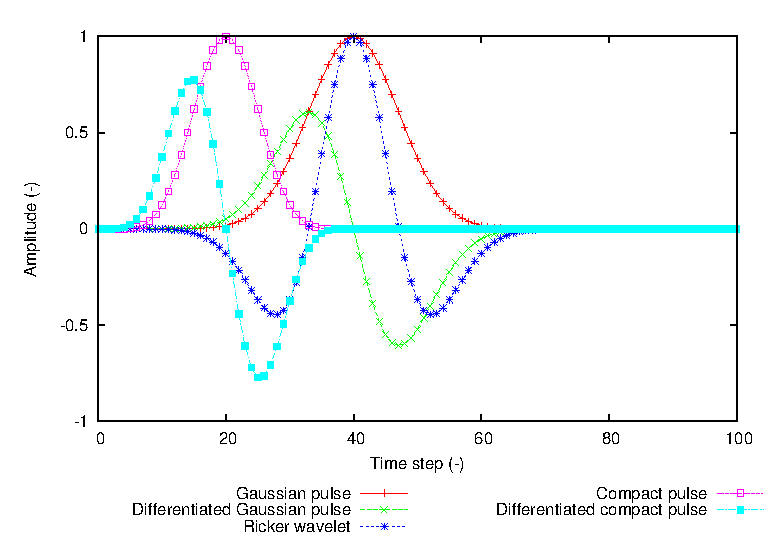
\includegraphics[width=0.9\linewidth]{figures/waveforms_td}
  \end{center}
  \caption{\label{fg:wfpulsetd}Default pulse waveforms and their derivatives.}
  \begin{center}
    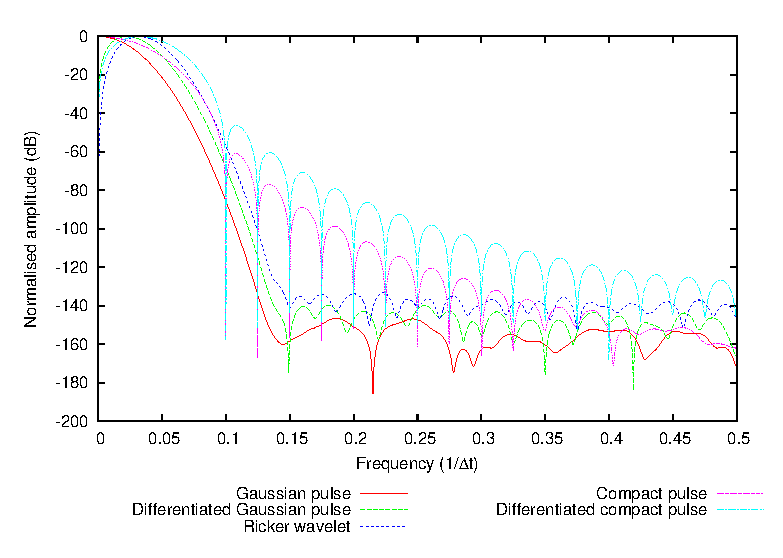
\includegraphics[width=0.9\linewidth]{figures/waveforms_fd}
  \end{center}
  \caption{\label{fg:wfpulsefd}Spectra of the pulse waveforms and their derivatives.}
\end{figure}

\begin{figure}[p]
  \begin{center}
    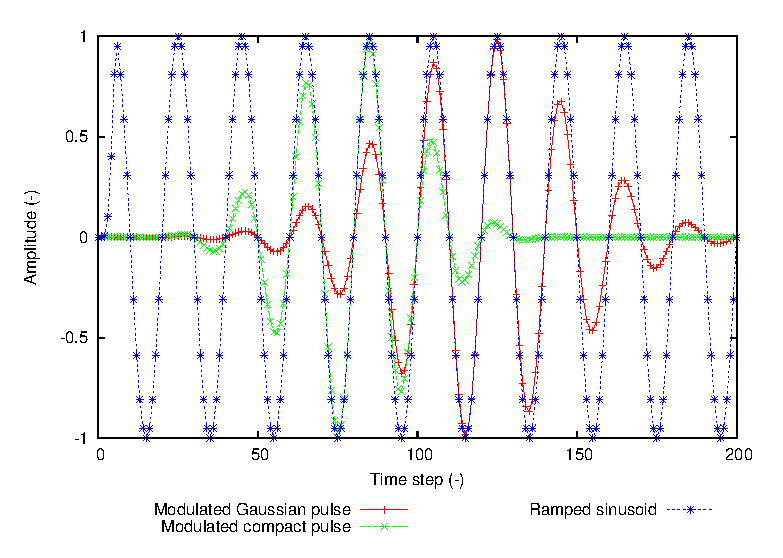
\includegraphics[width=0.9\linewidth]{figures/waveforms_mod_td}
  \end{center}
  \caption{\label{fg:wfmodtd}Default modulated waveforms.}
  \begin{center}
    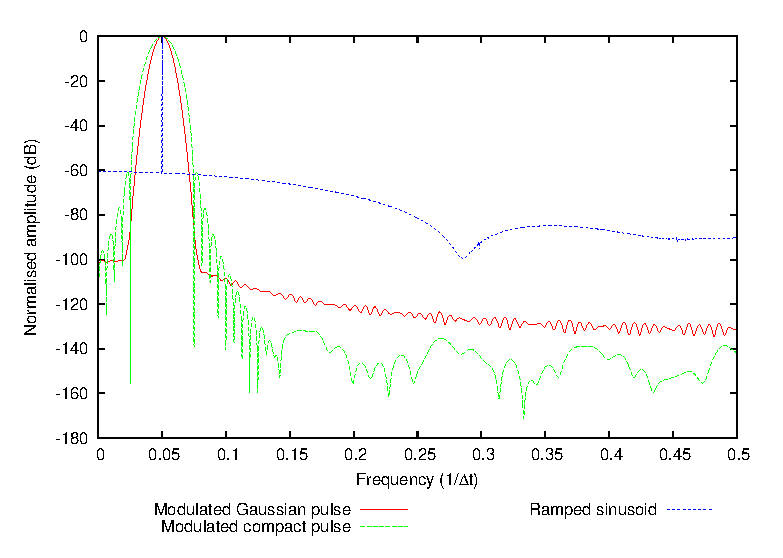
\includegraphics[width=0.9\linewidth]{figures/waveforms_mod_fd}
  \end{center}
  \caption{\label{fg:wfmodfd}Spectra of the default modulated waveforms.}
\end{figure}

\subsubsection{\texttt{EXTERNAL} waveform type}

A user defined waveform can be provided as a time-series in an external
ASCII file using the \texttt{EXTERNAL} waveform type:
\begin{verbatim}
WF <t: name> EXTERNAL <s: fileName> [ <r: size> [ <r: delay> ] ]
\end{verbatim}
\texttt{<s:~fileName>} is the path to an ASCII file containing two columns with monotonically increasing
time (seconds) and waveform values (-). The file format does not support any comment lines or blank lines!  The waveform 
is assumed zero outside the range of times in the file and is interpolated using cubic splines for 
values in between those given in the file. The waveform is scaled by
\texttt{<r:~size>} and delayed by \texttt{<r:~delay>} seconds.

% --
\subsection{Current and field sources: \texttt{EX}}
% --

Current and field sources are applied to the grid using the \texttt{EX} directive, 
which has two forms:
\begin{verbatim}
EX <i: ilo> <i: ihi> <i: jlo> <i: jhi> <i: klo> <i: khi> <t: name> <t: type> \
   <t: wfName> [ <r: size> [ <r: delay> ] ]
EX <i: ilo> <i: ihi> <i: jlo> <i: jhi> <i: klo> <i: khi> <t: name> <t: type> \
   <t: wfName> <r: param> [ <r: size> [ <r: delay> ] ]
\end{verbatim}
The first form is valid for all the distributed field and current sources while
the second form is used for lumped sources with finite internal impedance. 
Field and current sources are applied to the grid in the order they are defined
in the mesh file before any plane-wave sources.

The common source parameters are defined in Table~\ref{tb:exparm}. The waveform
to be used for the source, \texttt{<t:~wfName>}, must have been previously defined 
in a \texttt{WF} directive. The delay of the source relative to its waveform,
\texttt{<r:~delay>}, is {\em in addition to} any delay specified in the \texttt{WF} directive.

\begin{table}[ht]
\begin{center}
\begin{tabular}{|l|l|c|c|c|}
\hline
Parameter            &Quantity      &Symbol         &Units &Default \\ 
\hline
\texttt{<t:~name>}   &Source name   &n/a            &n/a   &none    \\ 
\texttt{<t:~type>}   &Source type   &n/a            &n/a   &none    \\ 
\texttt{<t:~wfName>} &Waveform name &n/a            &n/a   &$^*$    \\
\texttt{<r:~size>}   &Magnitude     &$A$            &$^*$  &1.0     \\
\texttt{<r:~delay>}  &Delay         &$t_\mathrm{d}$ &s     &0.0     \\ 
\hline
\end{tabular}
\caption{\label{tb:exparm}Source type common parameters. $^*$ depends on type.}
\end{center}
\end{table}

\subsection{Distributed ``soft`` current source types}

\begin{verbatim}
EX <i: ilo> <i: ihi> <i: jlo> <i: jhi> <i: klo> <i: khi> <t: name>  <t: type> \
   <t: wfName> [ <r: size> [ <r: delay> ] ]
\end{verbatim}

\begin{figure}[ht]
  \begin{center}
   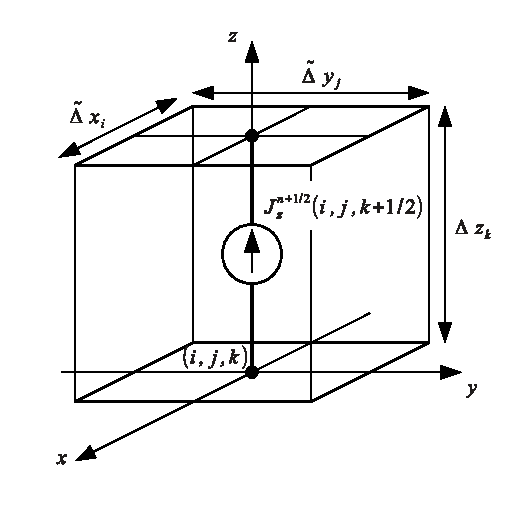
\includegraphics[width=0.4\linewidth]{figures/curr_src}
  \end{center}
  \vspace{-5mm}
  \caption{\label{fg:curr_src}Spatial region occupied by a soft electric current density source.}
\end{figure}

``Soft sources'' are added to the fields already on the computational
grid and as such do not cause reflections of waves scattered back towards them. 
Formally {\em all} such sources are ideal {\em current sources} with infinite impedance,
presenting an open-circuit to any waves incident upon them.
The field at the source location is the superposition of the incident field from the impressed
current and the scattered field (which may be the reaction of the grid to the incident field 
of the source itself or from another source in the grid).
The distributed soft sources supported are shown in Table~\ref{tb:exsoft}.
For surface current densities the first coordinate direction in the tag denotes the polarisation
direction of the current and the second denotes the other tangential direction of the current
sheet. So \texttt{JMSYZ} would denote a magnetic surface current density on an $x$-normal surface
polarised in the $y$-direction. For all other types the single coordinate direction in the tag 
denotes the polarisation, so \texttt{JY} would denote a $y$-polarised electric current density.

Electric current sources are excited on primary grid edges and magnetic current sources 
on secondary grid edges. Figure~\ref{fg:curr_src} shows the case of a $z$-polarised electric 
current density source on edge $[i,i,j,j,k,k+1]$. Note that the electric current is evaluated 
at half-intergral times $(n+\half) \Delta t$; magnetic currents are evaluated at integral times
$n \Delta t$.
For sources distributed over more than one edge the current density is distributed evenly over
the cross-sectional area of the source using parallel current sources and uniformly along the 
polarisation direction of the source using equal series current sources.
Essentially all the soft current sources excite the grid in the same way - the only difference
is the normalisation, and units, of the amplitude of the source. Depending on the type of
source been modelled one choice may be more natural than the other. If all outputs are
referenced to a calibration value measured on the computational grid then the amplitude
normalisation is unimportant. The normalisations for $z$-polarised electric current 
sources are
\begin{eqnarray}
J^{n+\half}_z(i,j,k+\half) 
= \mathtt{JZ} 
= \frac{\mathtt{JSZX}}{\tDelta y_j}
= \frac{\mathtt{JSZY}}{\tDelta x_i}  
= \frac{\mathtt{IZ}}{\tDelta x_i \tDelta y_j}
= \frac{\mathtt{IDZ}}{\tDelta x_i \tDelta y_j \Delta z_k}
= -\frac{\mathtt{EZ}}{\eta_0 c_0 \Delta t} 
= \frac{\mathtt{VZ}}{\eta_0 c_0 \Delta t  \Delta z_k}.
\end{eqnarray}
For an $x$-polarised magnetic current source the equivalent normalisation is
\begin{eqnarray}
J^{n+\half}_\mathrm{Mx}(i,j+\half,k+\half) 
= \mathtt{JMX} 
= \frac{\mathtt{JMSXY}}{\Delta z_k}
= \frac{\mathtt{JMSXZ}}{\Delta y_j}  
= \frac{\mathtt{IMX}}{\Delta y_j \Delta z_k}
= \frac{\mathtt{IMDX}}{\tDelta x_i \Delta y_j \Delta z_k}
= -\frac{\eta_0 \mathtt{HX}}{c_0 \Delta t}.
\end{eqnarray}
In the above, the normalisations for the fields and voltage assume that the source is imposed 
in free-space.

Note that isolated current sources in free-space often lead to permanent DC charging of the 
computational grid due to the lack of charge dynamics in the FDTD method. As a waveform is 
impressed by a current source the divergent fields implicitly displace charge between cells
in the grid according to the Gauss' Laws for electric and magnetic fields. This charging will
be temporary if the waveform has no DC component, however, for waveforms with DC components (like
a Gaussian pulse) a permanent static field will be left on the comptutational grid. If there 
is a conductive path between the end-points of the current source then the charge can discharge
with a time constant determined by the grid capacitance and conductance.

\begin{table}[ht]
\begin{center}
\begin{tabular}{|l|l|c|}\hline
Source type                                       &Description                        &Units       \\
\hline
\texttt{JX, JY, JZ}                               &Electric (volume) current density  &A\,m$^{-2}$ \\
\texttt{JMX, JMY, JMZ}                            &Magnetic (volume) current density  &V\,m$^{-2}$ \\
\texttt{JSXY, JSXZ, JSYZ, JSYX, JSZX, JSZY}       &Electric surface current density   &A\,m$^{-1}$ \\
\texttt{JMSXY, JMSXZ, JMSYZ, JMSYX, JMSZX, JMSZY} &Magnetic surface current density   &V\,m$^{-1}$ \\
\texttt{IX, IY, IZ}                               &Electric (line) current            &A           \\
\texttt{IMX, IMY, IMZ}                            &Magnetic (line) current            &V           \\
\texttt{IDX, IDY, IDZ}                            &Electric current moment            &A\,m        \\
\texttt{IMDX, IMDY, IMDZ}                         &Magnetic current moment            &V\,m        \\
\texttt{VX, VY, VZ}                               &Voltage                            &V           \\
\texttt{EX, EY, EZ}                               &Electric field                     &V\,m$^{-1}$ \\
\texttt{HX, HY, HZ}                               &Magnetic field                     &A\,m$^{-1}$ \\
\hline
\end{tabular}
\caption{\label{tb:exsoft}Distributed ``soft'' current source types. 1\,Wb = 1\,V\,s.}
\end{center}
\end{table}

\subsubsection{\texttt{JX}, \texttt{JY}, \texttt{JZ}, \texttt{JMX}, \texttt{JMY} and \texttt{JMZ} volume current density sources}

Volume current densities are applied directly to grid edges - primary grid edges for electric current densities and secondary grid 
edges for magnetic current densities. They can be regarded as existing across an area normal to their polarisation ditrection
given by the area of the dual grid faces associated with the edges excited.
For example,
\begin{verbatim}
# A soft electric current density source
EX 16 17 16 17 16 17 current_density JY 1.0
\end{verbatim}
would correspond to a $y$-polarised electric current density of 1\,A\,m$^{-2}$ impressed on four primary
grid edges in the volume bounded by \texttt{[15.5,17.5,15.5,17.5,16,17]}.

\subsubsection{\texttt{JSXY}, \texttt{JSXZ}, \texttt{JSYX}, \texttt{JSYZ}, \texttt{JSZX}, \texttt{JSZY},
\texttt{JMSXY}, \texttt{JMSXZ}, \texttt{JMSYX}, \texttt{JMSYZ}, \texttt{JMSZX}, \texttt{JMSZY} surface current density sources}
\label{sc:softsurfcur}

Surface current density sources are useful for impressing ``current sheet'' sources across surfaces of the grid. 
According to Love's Surface Equivalence Principle the sources within a surface
S can be replaced by the equivalent surface currents 
\begin{eqnarray}
\vJ_\mathrm{Ms} &=& -\left. \uvn \times \vE \right|_S \\
\vJ_\mathrm{s}  &=&  \left. \uvn \times \vH \right|_S
\end{eqnarray}
on the surface, leaving a null field inside the surface and the original
field outside the surface. An aperture in a PEC surface for 
example can be modelled using a magnetic surface current density 
$\vJ_\mathrm{Ms} = -\left. \uvn \times \vE \right|_S$
radiating on a PEC surface with the aperture closed (the electric current
density is shorted out in this case). The known electric
field in an aperture can be impressed using
\begin{verbatim}
# An equivalent magnetic current density source for an
# aperture with an electric field of 1 V/m.
TB  0 10 10 10  0 10 PEC
EX  5  6 10 10  5  6 aperture_efield JMSZY 1.0
\end{verbatim}
Note that this will radiate into both the $j<10$ and $j>10$ half-spaces which is 
probably not what is intended. A volumetic PEC backing needs to be used on the 
non-radiating side, say the $j<10$ half-space:
\begin{verbatim}
# An equivalent magnetic current density source for an
# aperture with a uniform electric field of 1 V/m.
MB  0 10  0 10  0 10 PEC
EX  5  6 10 10  5  6 aperture_efield JMSZY 1.0
\end{verbatim}

Another example is
\begin{verbatim}
# A soft electric surface current density source
EX 15 20 15 20 10 10 current_sheet JSXY 1.0
\end{verbatim}
which corresponds to an $x$-polarised electric surface current density of 1\,A\,m$^{-1}$ impressed on 36 primary
grid edges on the $z$-normal surface bounded by \texttt{[15,20,14.5,20.5,9.5,10.5]}. The equivalent volume current density
is determined by dividing surface current density by the dual grid edge length normal to the surface, 
in this case $\tDelta z_{10}$.

For infinitesimal sources that are not aligned with the grid it may be better to distributed the source over two edges
for each polarisation so that each polarisation has the same phase centre~\cite{Noetscher2012}. For example an electric
dipole moment with amplitude 1\,A\,m, aligned along unit vector $(1\sqrt{3},1\sqrt{3},1\sqrt{3})$ can be implemented using
\begin{verbatim}
# Non-aligned source with same phase centre for each polarisation.
EX 10 11 10 10 10 10 current_sheet IDX 0.5773
EX 10 10 10 11 10 10 current_sheet IDY 0.5773
EX 10 10 10 10 10 11 current_sheet IDZ 0.5773
\end{verbatim}

\subsubsection{\texttt{IX}, \texttt{IY}, \texttt{IZ}, \texttt{IMX}, \texttt{IMY} and \texttt{IMZ} line current sources}

Line current sources are related to current densities using the area of the dual grid face normal to and centred on the 
excited edge. For example, 
\begin{verbatim}
# A soft electric current source
EX 15 15 15 15 14 16 line_current IZ 1.0
\end{verbatim}
impresses a $z$-directed current of 1\, A flowing in the volume 
\texttt{[14.5,15.5,14.5,15.5,14,16]}. The current density is determined as
$1/(\tDelta x_{15} \tDelta y_{15})$\,A\,m$^{-2}$. Current sources can be specified
on volumetric bounding boxes as well. So,
\begin{verbatim}
# A soft volumetric electric current source
EX 15 16 15 16 14 16 line_current IZ 1.0
\end{verbatim}
would distribute the 1\,A current across the area $(\tDelta x_{15} + \tDelta x_{16})\times (\tDelta y_{15} + \tDelta y_{16}) $ 
normal to the current direction.

\subsubsection{\texttt{IDX}, \texttt{IDY}, \texttt{IDZ}, \texttt{IMDX}, \texttt{IMDY} and \texttt{IMDZ} current moment sources}

Current moments impress the specified current moment on a volume, surface or edge. The current
is determined by dividing the moment by the total length of the bounding box in the polarisation
direction and then the current density is found by dividing by the area of the normal dual grid
faces. For example,
\begin{verbatim}
# A soft volumetric electric current moment source
EX 15 16 15 16 14 16 current_moment IDZ 1.0
\end{verbatim}
would distribute the 1\,A\,m current moment across the area $(\tDelta x_{15} + \tDelta x_{16})\times (\tDelta y_{15} + \tDelta y_{16}) $ 
normal to the current direction and length $\Delta z_{14}+\Delta x_{15}$.

\subsubsection{\texttt{EX}, \texttt{EY}, \texttt{EZ}, \texttt{HX}, \texttt{HY} and \texttt{HZ} soft ``field'' sources}

Soft ``field'' sources are added directly to the fields already on the grid, however, as noted above they
are formally {\em current sources} with respect to their physical behaviour. The field they impress on the grid
is dependent on the time-step (and hence CFLN). In general this means they are difficult to use on a
non-uniform mesh. In Vulture the soft electric field source is normalised such that on a uniform grid with the
default CFLN of $\sqrt{3}/2$ an infinite plane of colinearly polarised edges would launch a plane 
wave with the specified electric/magnetic field amplitude in to the grid. Explicitly,
\begin{verbatim}
# A soft electric ``field'' source
EX  1 10  1 10  5  5 eplane EZ 1.0
\end{verbatim}
would launch a ``plane-wave'' of amplitude 1\,V/m in both the positve and negative $z$-directions
on a uniform mesh with the default CFLN. {\em Note that in practice the source plane is usually not infinite 
and therefore this give a poor representation of a plane-wave:} There will be always be diffraction 
from the edges of the source plane. However, within an infinite parallel-plate waveguide, simulated using
PEC and PMC external boundaries, the source plane is effectively infinite and in this case a well defined
TEM wave is launched (in both directions). The PEC external boundaries also effectively remove any displaced charge from the
grid and prevent DC charging of the grid for this case too.

\subsubsection{\texttt{VX}, \texttt{VY} and \texttt{VZ} soft ``voltage'' sources}

Soft voltage sources are just soft field sources normalised by the total edge length of 
the bounding box in the direction of polarisation, so all the comments above for field sources 
apply equally here.

\subsection{Distributed ``hard`` field source types}

\begin{verbatim}
EX <i: ilo> <i: ihi> <i: jlo> <i: jhi> <i: klo> <i: khi> <t: name>  <t: type> \
   <t: wfName> [ <r: size> [ <r: delay> ] ]
\end{verbatim}

\begin{figure}[ht]
  \begin{center}
   \includegraphics[width=0.4\linewidth]{figures/volt_src}
  \end{center}
  \vspace{-5mm}
  \caption{\label{fg:volt_src}Spatial region occupied by a hard electric field source.}
\end{figure}

``Hard sources'' replace the fields already on the computational
grid and as such cause reflections of waves scattered back towards them. 
Formally such sources are ideal {\em voltage sources} with zero impedance,
presenting a short-circuit to any waves incident upon them.
For sources distributed over more than one edge the voltage is distributed uniformly over
the cross-sectional area of the source using equal parallel voltage sources and evenly 
along the polarisation direction of the source using series voltage sources.
The edges on which hard sources are impressed appear as PEC or PMC materials
as far as waves scattering from them are concerned. Indeed, one practical
use of a hard source is to impress the equivalent surface currents of an 
aperture field onto a PEC surface, however, it must always be bourne in mind
that any waves reflected back towards such a source may suffer unphysical 
reflections. This is discussed futher below.
The distributed hard sources supported are shown in Table~\ref{tb:exsoft}.

Electric sources are excited on primary grid edges (centres of secondary grid faces) 
and magnetic sources at the centres of primary grid faces (on secondary grid edges). 
Figure~\ref{fg:volt_src} shows the case of a $z$-polarised hard electric 
field source on edge $[i,i,j,j,k,k+1]$. Note that electric field sources are evaluated 
at intergral times $n \Delta t$; magnetic field sources are evaluated at half-integral times
$(n+\half) \Delta t$.
Essentially all the hard field sources excite the grid in the same way - the only difference
is the normalisation, and units, of the amplitude of the source. Depending on the type of
source been modelled one choice may be more natural than the other. If all outputs are
referenced to a calibration value measure on the computational grid then the amplitude
normalisation is unimportant. The normalisations for a $z$-polarised hard electric
field source are
\begin{eqnarray}
E^{n+\half}_z(i,j,k+\half) 
&=& \mathtt{EZ}
= -\frac{\mathtt{VZ}}{\Delta z_k}
= -\eta_0 c_0 \Delta t \mathtt{JZ}
= -\eta_0 c_0 \Delta t \frac{\mathtt{JSZX}}{\tDelta y_j}
= -\eta_0 c_0 \Delta t \frac{\mathtt{JSZY}}{\tDelta x_i} \nonumber \\
&=& -\eta_0 c_0 \Delta t \frac{\mathtt{IZ}}{\tDelta x_i \tDelta y_j}
= -\eta_0 c_0 \Delta t \frac{\mathtt{IDZ}}{\tDelta x_i \tDelta y_j \Delta z_k}
\end{eqnarray}
For an $x$-polarisaed hard magnetic field source the equivalent normalisation is
\begin{eqnarray}
H^{n+\half}_\mathrm{x}(i,j+\half,k+\half) 
&=& \mathtt{HX}
= -\frac{c_0 \Delta t}{\eta_0}\mathtt{JMX}
= -\frac{c_0 \Delta t}{\eta_0}\frac{\mathtt{JMSXY}}{\Delta z_k}
= -\frac{c_0 \Delta t}{\eta_0}\frac{\mathtt{JMSXZ}}{\Delta y_j} \nonumber \\
&=& -\frac{c_0 \Delta t}{\eta_0}\frac{\mathtt{IMX}}{\Delta y_j \Delta z_k}
= -\frac{c_0 \Delta t}{\eta_0}\frac{\mathtt{IMDX}}{\tDelta x_i \Delta y_j \Delta z_k}.
\end{eqnarray}
The above the normalisations for the fields and voltage assume that the source is imposed 
in free-space. Note that the fields induced on the grid for all the current related hard sources
depend on the time-step (and CFLN).

\begin{table}[ht]
\begin{center}
\begin{tabular}{|l|l|c|}\hline
Source type                                             &Description                        &Units       \\
\hline
\texttt{=EX, =EY, =EZ}                                  &Electric field                     &V\,m$^{-1}$ \\
\texttt{=HX, =HY, =HZ}                                  &Magnetic field                     &A\,m$^{-1}$ \\
\texttt{=VX, =VY, =VZ}                                  &Voltage                            &V           \\
\texttt{=JX, =JY, =JZ}                                  &Electric (volume) current density  &A\,m$^{-2}$ \\
\texttt{=JMX, =JMY, =JMZ}                               &Magnetic (volume) current density  &V\,m$^{-2}$ \\
\texttt{=JSXY, =JSXZ, =JSYZ, =JSYX, =JSZX, =JSZY}       &Electric surface current density   &A\,m$^{-1}$ \\
\texttt{=JMSXY, =JMSXZ, =JMSYZ, =JMSYX, =JMSZX, =JMSZY} &Magnetic surface current density   &V\,m$^{-1}$ \\
\texttt{=IX, =IY, =IZ}                                  &Electric (line) current            &A           \\
\texttt{=IMX, =IMY, =IMZ}                               &Magnetic (line) current            &V           \\
\texttt{=IDX, =IDY, =IDZ}                               &Electric current moment            &A\,m        \\
\texttt{=IMDX, =IMDY, =IMDZ}                            &Magnetic current moment            &V\,m        \\
\hline
\end{tabular}
\caption{\label{tb:exhard}Distributed ``hard'' field source types.}
\end{center}
\end{table}

\subsubsection{\texttt{=EX}, \texttt{=EY}, \texttt{=EZ}, \texttt{=HX}, \texttt{=HY} and \texttt{=HZ} hard field sources}

Hard field source can be used to impress known field distributions on surfaces, similar to the use
of current sheets in Section~\ref{sc:softsurfcur} above. With a hard source an aperture field can be imposed directly
on a PEC surface, for example:
\begin{verbatim}
# Direct Dirchlet boundary condition for
# aperture with a uniform electric field of 1 V/m.
MB  0 10  0 10  0 10 PEC
EX  5  6 10 10  5  6 aperture_efield =EZ 1.0
\end{verbatim}

\subsubsection{\texttt{=VX}, \texttt{=VY} and \texttt{=VZ} hard voltage sources}

Hard voltage sources are just hard field sources normalised by the total edge length of 
the bounding box in the direction of polarisation. They can be used in cases where
an ideal voltage source excitation is required.

\subsubsection{\texttt{=JX}, \texttt{=JY}, \texttt{=JZ}, \texttt{=JMX}, \texttt{=JMY} and \texttt{=JMZ} hard 
current density sources}

These source types are provided for completeness but may not be practically useful.

\subsubsection{\texttt{=JSXY}, \texttt{=JSXZ}, \texttt{=JSYX}, \texttt{=JSYZ}, \texttt{=JSZX}, \texttt{=JSZY},
\texttt{=JMSXY}, \texttt{=JMSXZ}, \texttt{=JMSYX}, \texttt{=JMSYZ}, \texttt{=JMSZX}, \texttt{=JMSZY} hard surface current density sources}

These source types can be used to impose current sheets, however, the field induced on the mesh is dependent on the
time-step and will only have the correct normalisation on uniform cubic grids with the default CFLN. It is usually
better to imposed field values directly using \texttt{=EX} etc.

\subsubsection{\texttt{=IX}, \texttt{=IY}, \texttt{=IZ}, \texttt{=IMX}, \texttt{=IMY} and \texttt{=IMZ} hard 
current sources}

These source types are provided for completeness but may not be practically useful.

\subsubsection{\texttt{=IDX}, \texttt{=IDY}, \texttt{=IDZ}, \texttt{=IMDX}, \texttt{=IMDY} and \texttt{=IMDZ} hard 
current moment sources}

These source types are provided for completeness but may not be practically useful.

\subsection{Other source types}

\subsubsection{\texttt{VRX}, \texttt{VRY}, \texttt{VRZ}, \texttt{IRX}, \texttt{IRY} and \texttt{IRZ} finite impedance lumped sources}

\begin{verbatim}
EX <i: ilo> <i: ihi> <i: jlo> <i: jhi> <i: klo> <i: khi> <t: name> VRX|VRY|VRZ|IRX|IRY|IRZ \
   <t: wfName> <r: resist> [ <r: size> [ <r: delay> ] ]
\end{verbatim}

\begin{figure}[ht]
  \begin{center}
   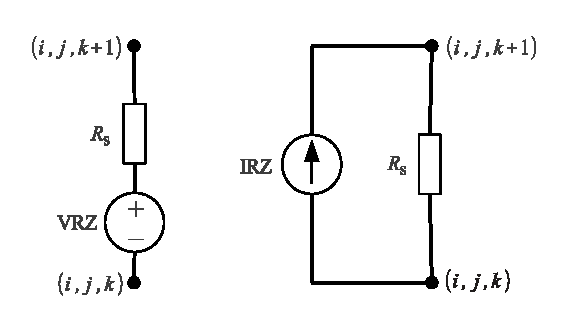
\includegraphics[width=0.4\linewidth]{figures/lumped_src}
  \end{center}
  \vspace{-5mm}
  \caption{\label{fg:lumped_src}Schematic illustration of lumped Th{\'e}venin voltage source (left)
  and Norton current source (right) on a $z$-polarised edge.}
\end{figure}

This form of the \texttt{EX} directive is used to introduce lumped Th{\'e}venin voltage and
Norton current sources with finite internal impedance. For Th{\'e}venin voltage sources
the amplitude \texttt{<r:~size>} is the open circuit voltage of the source in volts and
\texttt{<r:~resist>} is the internal resistance in ohms. For Norton current sources
the amplitude \texttt{<r:~size>} is the short circuit current of the source in amps and
\texttt{<r:~resist>} is the internal resistance in ohms. Both sources are implement as soft 
current sources on the corresponding electric field edge, together with an appropriate
conductive loading of the edge to account for the source resistance, as shown in Figure~\ref{fg:lumped_src}.
Currently the bounding box must be a single edge!

Examples:
\begin{verbatim}
# A soft z-polarised lumped voltage source of ampltiude 1 V
# and internal resistance 50 ohms applied on the grid edge 
# from (16,16,16) to (16,16,17).
EX 16 16 16 16 16 17 feed VRZ 50.0 1.0
\end{verbatim}

\subsubsection{\texttt{VDX}, \texttt{VDY} and \texttt{VDZ} delta-gap thin wire voltage sources}

{\color{red}\it Delta-gap sources are currently not implemented!\\ \\}

% --
\subsection{Plane-wave sources: \texttt{PW}}
% --

Plane-waves can be launched into the computational grid using the
\texttt{PW} directive:
\begin{verbatim}
PW <i: ilo> <i: ihi> <i: jlo> <i: jhi> <i: klo> <i: khi> <t: name> <t: wfName> \
   <r: theta> <r: phi> <r: psi> [ <s: mask> [<r: size> [ <r: delay> ] ] ]
\end{verbatim}
Plane-wave sources partition the grid into two regions:
\begin{itemize}
 \item A total field region inside of the bounding box.
 \item A scattered field region outside of the bounding box.
\end{itemize}
Such source are also known as Huygen's sources or total-field
scattered-field (TFSF) sources or boundaries. The bounding box must 
define a volume and {\em must not cut across any objects on the mesh}; it can
however butt-up against an internal PEC surface or external PEC, PMC or PERIODIC 
surface in certain cases (see \texttt{<t:~mask>} below).
Plane-wave sources are applied in the order they are given in the mesh file
after all other types of sources.

\begin{table}[ht]
\begin{center}
\begin{tabular}{|l|l|c|c|c|}
\hline
Parameter            &Quantity           &Symbol         &Units   &Default \\ 
\hline
\texttt{<t:~name>}   &Plane-wave name    &n/a            &n/a     &none    \\
\texttt{<t:~wfName>} &Waveform name      &n/a            &n/a     &none    \\
\texttt{<r:~theta>}  &Polar angle        &$\theta$       &degrees &none    \\
\texttt{<r:~phi>}    &Azimuthal angle    &$\phi$         &degrees &none    \\
\texttt{<r:~psi>}    &Polarisation angle &$\psi$         &degrees &none    \\
\texttt{<t:~mask>}   &Face activity mask &n/a            &n/a     &111111  \\
\texttt{<r:~size>}   &Magnitude          &$E_0$          &V/m     &1.0     \\
\texttt{<r:~delay>}  &Delay              &$t_\mathrm{d}$ &s       &0.0     \\ 
\hline
\end{tabular}
\caption{\label{tb:pwparm}Plane-wave source type parameters.}
\end{center}
\end{table}

The plane-wave source type parameters are:
\begin{itemize}
 \item \texttt{<t:~name>}: The unique name of the plane-wave.
 \item \texttt{<t:~wfName>}: The name of the waveform to use for the source. 
 This must have been defined already in a \texttt{WF} directive.
 \item \texttt{<r:~theta>}: The polar angle, $0 \le \theta \le 180$, of the wave vector in degrees.
 \item \texttt{<r:~phi>}: The azimuthal angle, $0 \le \phi < 360$, of the wave vector in degrees.
 \item \texttt{<r:~psi>}: The polarisation angle, $0 \le \psi \le 360$, of the electric field vector relative
 to $\hat{\mathbf{k}}^\mathrm{inc} \mathbf{\times} \hat{\mathbf{z}}$ in degrees.
 \item \texttt{<s:~mask>}: A bit mask of six binary digits indicating which faces
 (\texttt{XLO XHI YLO YHI ZLO ZHI}) of the plane-wave bounding box are active. e.g \texttt{111111}
 indicates all faces are active while \texttt{011111} indicates that the \texttt{XLO} face is inactive. 
 This can be used to terminate one face (the inactive one) of the TFSF surface with a PEC plate to
 construct a semi-infinite space. The reflected wave must be included using a second \texttt{PW}
 directive with opposite wave-vector and polarisation in this case to obtain accurate results - see the examples later.
 \item \texttt{<r:~size>}: The source amplitude, $E_0$, in V/m. The default 
 value is 1.0 V/m. 
 \item \texttt{<r:~delay>}: The delay of the source relative to the waveform in seconds. This
 delay is in addition to any delay specified in the \texttt{WF} directive.
\end{itemize}
These parameters are summarised in Table~\ref{tb:pwparm} and Figure~\ref{fg:pw} shows how the angles are 
defined. The incident wave-vector, electric field vector and magnetic field vector are given by 
\begin{eqnarray}
\hat{\mathbf{k}}^\mathrm{inc} = \hat{\mathbf{r}}
=  \left[
\begin{array}{c}
\sin( \theta ) \cos( \phi ) \\
\sin( \theta ) \sin( \phi ) \\
\cos( \theta )
\end{array}
\right]
\label{eq:kinc}
\end{eqnarray}
\begin{eqnarray}
\mathbf{E}^\mathrm{inc}
= E_0 \left[
\begin{array}{c}
 \cos( \psi ) \sin( \phi ) - \sin( \psi ) \cos( \theta ) \cos( \phi ) \\
-\cos( \psi ) \cos( \phi ) - \sin( \psi ) \cos( \theta ) \sin( \phi ) \\
 \sin( \psi ) \sin( \theta )
\end{array}
\right]
\label{eq:Einc}
\end{eqnarray}
\begin{eqnarray}
\mathbf{H}^\mathrm{inc}
= \frac{E_0}{\eta_0} \left[
\begin{array}{c}
 \sin( \psi ) \sin( \phi ) + \cos( \psi ) \cos( \theta ) \cos( \phi ) \\
-\sin( \psi ) \cos( \phi ) + \cos( \psi ) \cos( \theta ) \sin( \phi ) \\
-\cos( \psi ) \sin( \theta )
\end{array}
\right].
\label{eq:Hinc}
\end{eqnarray}
The angles for common directions and polarisations are given in Table~\ref{tb:pwangles}. 

\begin{figure}[ht]
  \begin{center}
   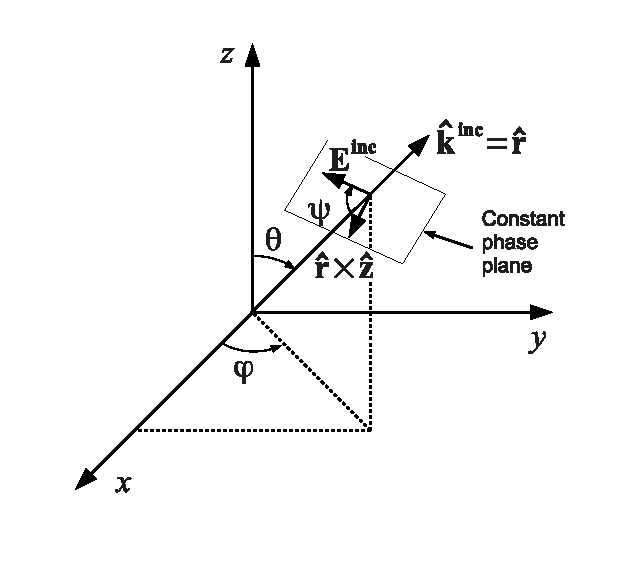
\includegraphics[width=0.4\linewidth]{figures/planewave}
  \end{center}
  \caption{\label{fg:pw}Definition of the angles of the wave-vector and electric field vector for the plane-wave source.}
\end{figure}

\begin{table}[ht]
\begin{center}
\begin{tabular}{|c|c|c|c|c|c|}
\hline
$\hat{\mathbf{k}}^\mathrm{inc}$ &$\hat{\mathbf{E}}^\mathrm{inc}$ &$\hat{\mathbf{H}}^\mathrm{inc}$ 
&$\theta\,(^\circ)$             &$\phi\,(^\circ)$                &$\psi\,(^\circ)$                \\  
\hline
$k_x \hat{\mathbf{x}}$          &$E_y \hat{\mathbf{y}}$          &$H_z \hat{\mathbf{z}}$    
&90                             &0                               &180                             \\
$k_x \hat{\mathbf{x}}$          &$E_z \hat{\mathbf{z}}$          &$H_y \hat{\mathbf{y}}$    
&90                             &0                               &90                              \\
$k_y \hat{\mathbf{y}}$          &$E_x \hat{\mathbf{x}}$          &$H_z \hat{\mathbf{z}}$    
&90                             &90                              &0                               \\
$k_y \hat{\mathbf{y}}$          &$E_z \hat{\mathbf{z}}$          &$H_x \hat{\mathbf{x}}$    
&90                             &90                              &90                              \\
$k_z \hat{\mathbf{z}}$          &$E_x \hat{\mathbf{x}}$          &$H_y \hat{\mathbf{y}}$    
&0                              &0                               &270                             \\
$k_z \hat{\mathbf{z}}$          &$E_y \hat{\mathbf{y}}$          &$H_x \hat{\mathbf{x}}$    
&0                              &0                               &180                             \\
$-k_x \hat{\mathbf{x}}$         &$-E_y \hat{\mathbf{y}}$         &$H_z \hat{\mathbf{z}}$    
&90                             &180                             &180                             \\
$-k_x \hat{\mathbf{x}}$         &$-E_z \hat{\mathbf{z}}$         &$-H_y \hat{\mathbf{y}}$    
&90                             &180                             &270                             \\
$-k_y \hat{\mathbf{y}}$         &$-E_x \hat{\mathbf{x}}$         &$-H_z \hat{\mathbf{z}}$    
&90                             &270                             &0                               \\
$-k_y \hat{\mathbf{y}}$         &$-E_z \hat{\mathbf{z}}$         &$H_x \hat{\mathbf{x}}$    
&90                             &270                             &270                             \\
$-k_z \hat{\mathbf{z}}$         &$-E_x \hat{\mathbf{x}}$         &$H_y \hat{\mathbf{y}}$    
&180                            &0                               &270                             \\
$-k_z \hat{\mathbf{z}}$         &$-E_y \hat{\mathbf{y}}$         &$-H_x \hat{\mathbf{x}}$    
&180                            &0                               &0                               \\
\hline
\end{tabular}
\caption{\label{tb:pwangles}Angles for common directions of propagation and polarisation.}
\end{center}
\end{table}

On a cubic mesh an auxiliary 1D grid is used to accurately account for dispersion across the total field
region. On non-cubic uniform meshes and non-uniform meshes a basic analytic incident field is used: This 
has low accuracy on electrically large meshes. In any case it is advisable to make the plane-wave bounding
box as small as possible to minimise any dispersion errors.

%
% ----------------------------------------------------------------------- 
%
\section{Observers}
\label{sc:obs}
%
% ----------------------------------------------------------------------- 
%

{\color{red}\it The observer directive format and assocaited output file formats are under review and may change in a future version of Vulture.}

% --
\subsection{Simulation output control: \texttt{OT}, \texttt{OF}}
% --

The \texttt{OT} directive determines for which time-steps data are output by the time-domain observers:
\begin{verbatim}
OT <i: tstart> <i: tstop>
\end{verbatim}
The data for all time-steps between and including  \texttt{<i:~tstart>} and  \texttt{<i:~tstop>} will be
written out. By default the data for all time-steps is output if no \texttt{OT} directive is given.

For frequency domain observers, including waveforms and far-fields calculations, the frequencies to be output
are determined by the \texttt{OF} directive:
\begin{verbatim}
OF <r: fstart> <r: fstop> <i: numFreq>
\end{verbatim}
By default,  if no \texttt{OF} directive is given, the frequencies  
\begin{eqnarray}
f_k  = \frac{k}{N_\mathrm{s}\Delta t}\,\,\,\,\,k=0,\ldots,\frac{N_\mathrm{s}}{10}
\end{eqnarray}
are output, where $N_\mathrm{s}$ is the number of time-steps and $\Delta t$ is the time-step.
The DFTs are computed using the time-series within the bounds specified by any \texttt{OT} directive
or the full time series if there is no \texttt{OT} directive.

% --
\subsection{Implicit waveform observers}
% --
% 

For every waveform directive found in the mesh file two implicit ```waveform observers'' are
automatically created which monitor the waveform's time-series and frequency spectrum. 
Waveform time-series are output into ASCII files called \texttt{wf\_<t:~name>\_td.asc}, where 
\texttt{<t:~name>} is the name of the waveform in the mesh-file. The associated frequency
spectra are similarly stored in ASCII files called \texttt{wf\_<t:~name>\_fd.asc}. The
output format are given in Tabe~\ref{tb:opwf}.

\begin{table}[th]
{\footnotesize
\begin{Verbatim}[frame=single]
# Waveform# 0
# ts (-)            t (s)           wf (-)
       0   0.00000000e+00   0.00000000e+00    
       .   ..............   ..............
\end{Verbatim}
\begin{Verbatim}[frame=single]
# Waveform# 0
#         f (Hz)       Re(wf) (-)       Im(wf) (-)
  0.00000000e+00   0.00000000e+00   0.00000000e+00
  ..............   ..............   ..............
\end{Verbatim}
}
\caption{\label{tb:opwf} Output formats for implicit waveform obserbvers: Time series (top) and frequency spectra (bottom).}
\end{table}

% --
\subsection{Near-field observers: \texttt{OP}}
% --

Near-field output requests are made using \texttt{OP} directives which have two forms depending on the type:
\begin{verbatim}
OP <i: ilo> <i: ihi> <i: jlo> <i: jhi> <i: klo> <i: khi> <t: name> <t: type> \
   [ <t: wfName> ]
OP <i: ilo> <i: ihi> <i: jlo> <i: jhi> <i: klo> <i: khi> <t: name> <t: type> \
   [ <i: xstep> <i: ystep> <i: zstep> ] ]
\end{verbatim}
These directives place observers on the computational grid that output the fields on and within 
the specified bounding box. 

\subsubsection{\texttt{TDOM\_BINARY} type observers}

\begin{verbatim}
OP <i: ilo> <i: ihi> <i: jlo> <i: jhi> <i: klo> <i: khi> <t:name> TDOM_BINARY \
   [ <i: xstep> <i: ystep> <i: zstep> ]
\end{verbatim}

The \texttt{TDOM\_BINARY} type requests time-domain field outputs over a volumetric region in the 
University of York finite methods binary output format~\cite{procman}. The electric and
magnetic field components in each cell enclosed by the bounding box are output with a cell index stride 
length in each coordinate direction given by \texttt{<i:~xstep>}, \texttt{<i:~ystep>} and \texttt{<i:~zstep>}.
The default stride lengths are one in all directions. The time-series of the first waveform defined in the
mesh file will be stored in the \texttt{excite.dat} to be used as a reference in frequency domain calculations.

The observer outputs are indexed by cell numbers but are sampled at their respective positions and times in 
the Yee cell shown in Figure~\ref{fg:yeecell}. For example \texttt{Ex[i][j][k]} is sampled at position 
$(x_i + \frac{dx_i}{2} , y_j , z_k )$ and \texttt{Hx[i][j][k]} is sampled at position 
$(x_i , y_j + \frac{dy_j}{2}, z_k + \frac{dz_k}{2} )$. Time domain fields are output with electric field times. 
The magnetic fields are half a time step later than the time specified. 

Frequency domain outputs are divided by the spectrum of the (complex) reference waveform, defined by 
the \texttt{<t:~wfName>} parameter, to give the frequency response of the observerable
relative to the source waveform. Any amplitude factor in the waveform directive is therefore divided out, however,
amplitude factors in excitation directives are retained. The default reference waveform is the first one found in mesh. 
Magnetic field spectra have a phase shift (advance) corresponding to half a time step.

The results are stored in a binary output file called \texttt{impulse.dat}. Results from multiple
\texttt{TDOM\_BINARY} types observers are stored in the same \texttt{impulse.dat} file. Two other
files are also created when \texttt{TDOM\_BINARY} type observers are present: 
\begin{itemize}
 \item \texttt{excite.dat}: An ASCII file containing the reference excitation waveform time series.
 \item \texttt{process.dat}: A template ASCII file for controlling other post processing tools.
\end{itemize}
See Section~\ref{sc:binarypp} for information on using the binary output data. Note that the name tag is currently
not propagated in to the output data files.

For example the directive 
\begin{verbatim}
OP  4 10 14 20 10 10 output1 TDOM_BINARY 2 2 1
\end{verbatim}
will output electric and magnetic fields on a 2D grid of cells with 
\begin{itemize}
 \item $x$ indices 4, 6, 8 and 10.
 \item $y$ indices 14, 16, 18 and 20. 
 \item $z$ index 10. 
\end{itemize}

\subsubsection{\texttt{TDOM\_ASCII} and \texttt{FDOM\_ASCII} type observers}

\begin{verbatim}
OP <i: ilo> <i: ihi> <i: jlo> <i: jhi> <i: klo> <i: khi> <t: name> TDOM_ASCII
OP <i: ilo> <i: ihi> <i: jlo> <i: jhi> <i: klo> <i: khi> <t: name> FDOM_ASCII [ <t: wfName> ]
\end{verbatim}

The \texttt{TDOM\_ASCII} and \texttt{FDOM\_ASCII} observer types requests time-domain and 
frequency-domain ASCII format field outputs respectively in a single mesh cell. As such the 
bounding box {\em must} be a single cell. 

Time-domain outputs for each observer of type \texttt{TDOM\_ASCII} are written to separate files 
with names \texttt{eh\_<t:~name>\_td.asc}. The file format is given in Table~\ref{tb:opasctd}.
The outputs are sampled at their respective positions and times in the Yee cell shown in 
Figure~\ref{fg:yeecell}. For example \texttt{Ex[i][j][k]} is sampled 
at position  $(x_i + \frac{dx_i}{2} , y_j , z_k )$ and \texttt{Hx[i][j][k]} is sampled at position 
$(x_i , y_j + \frac{dy_j}{2}, z_k + \frac{dz_k}{2} )$. Time domain fields are output with electric field times. 
The magnetic fields are half a time step later than the time specified. 

Frequency-domain outputs for each observer of type \texttt{FDOM\_ASCII} are written to separate 
files with names \texttt{eh\_<t:~name>\_fd,asc}. The file format is given in Table~\ref{tb:opascfd}.
Frequency domain outputs are divided by the spectrum of the (complex) reference waveform, defined by 
the \texttt{<t:~wfName>} parameter, to give the frequency response of the observerable
relative to the source waveform. Any amplitude factor in the waveform directive is therefore divided out, however,
amplitude factors in excitation directives are retained. If no reference waveform is given the first one found 
in the mesh file is used. Magnetic field spectra have a phase shift corresponding to half a time step.

\begin{table}[th]
{\footnotesize
\begin{Verbatim}[frame=single]
# [<i: ilo>,<i: jlo>,<i: klo>] -> (x_ilo,y_jlo,z_klo)
# ts (-)            t (s)         Ex (V/m)         Ey (V/m)         Ez (V/m)         Hx (A/m) ...
       0   0.00000000e+00   0.00000000e+00   0.00000000e+00   0.00000000e+00   0.00000000e+00 ... 
       .   ..............   ..............   ..............   ..............   .............. ...
\end{Verbatim}
}
\caption{\label{tb:opasctd} Output format of the \texttt{TDOM\_ASCII} observer types.}
\end{table}

\begin{table}[th]
{\footnotesize
\begin{Verbatim}[frame=single]
# [<i: ilo>,<i: jlo>,<i: klo>] -> (x_ilo,y_jlo,z_klo)
#         f (Hz)     Re(Ex) (V/m)     Im(Ex) (V/m)     Re(Ey) (V/m)     Im(Ey) (V/m)  ...
  0.00000000e+00   0.00000000e+00   0.00000000e+00   0.00000000e+00   0.00000000e+00  ...
  ..............   ..............   ..............   ..............   ..............  ...
\end{Verbatim}
}
\caption{\label{tb:opascfd} Output format of the \texttt{FDOM\_ASCII} observer types.}
\end{table}

\subsubsection{\texttt{HDF5} type observers}

{\color{red}\it HDF5 observers are currently not implemented!\\ \\}

\begin{verbatim}
OP <i: ilo> <i: ihi> <i: jlo> <i: jhi> <i: klo> <i: khi> <t: name> TDOM_HDF5 [<t: wfName>]
\end{verbatim}

These will have the following characteristics:
\begin{itemize}
 \item Nodal observers.
 \item All outputs to one file called \texttt{output.h5}.
 \item Maybe AMELET format.
 \item Optional compilation using \texttt{USE\_HDF5=ON/OFF}.
\end{itemize}

% --
\subsection{Far-field observers: \texttt{FF}}
% --

{\color{red}\it Far-field observers are currently not implemented!\\ \\}

{\color{red}
The \texttt{FF} directive requests a near-field to far-field transformation of the 
fields over the bounding box:
\begin{verbatim}
FF <i: ilo> <i: ihi> <i: jlo> <i: jhi> <i: klo> <i: khi> <t: name> <t: wfName> \
   <r: theta1> <r: theta2> <i: num_theta> <r: phi1> <r: phi2> <i: num_phi> [ <t: mask> ]
\end{verbatim}

These will have the following characteristics:
\begin{itemize}
 \item Calculate the frequency domain far-field from the near-field sampled on the bounding box.
 \item Calculate the total radiated power in far field by integrating the pattern.
 \item Calculate the frequency domain power flowing out of the bounding box by integrating the
 Poynting flux.
 \item Check the power balance between the previous two powers.
 \item Use a running DFT via ``internal'' surface observers.
 \item Use frequencies from the OF card or those automatically determined.
 \item The bounding box must be a volume.
 \item \texttt{<r:~theta1>}: Start polar angle in degrees [0,180).
 \item \texttt{<r:~theta2>}: Stop polar angle in degrees (0,180), $>=$ \texttt{r:~theta1}
 \item \texttt{<i:~num\_theta>}: Number of polar angles, $>=$ 0.
 \item \texttt{<r:~phi1>}: Start azimuthal angle in degrees [0,360).
 \item \texttt{<r:~phi2>}: Stop azimuthal angle in degrees (0,360], $>=$ \texttt{r:~phi1}.
 \item \texttt{<i: num\_phi>}: Number of azimuthal angles, $>=$ 0.
 \item \texttt{<t:~mask>} is a bitmap that defines which faces (XLO XHI YLO YHI ZLO ZHI) are included e.g 111111, 011111.
 \item Origin is the centre of bounding box - may need to make it a parameter?
 \item Phase reference - is the waveform? Distance for phase calculation?
 \item Output is $\theta$, $\phi$, $E_\theta$, $E_\phi$, power gain/RCS 
 in files called \texttt{rcs\_<i:~freqNum>.asc} where \texttt{<i:~freqNum>} is the frequency number.
\end{itemize}
}

%
% ----------------------------------------------------------------------- 
%
\section{Viewing the mesh}
%
% ----------------------------------------------------------------------- 
%

% --
\subsection{\texttt{gvulture}}
% --

The program \texttt{gvulture} converts a Vulture mesh into a set of files suitable for 
3D viewing of the mesh using Gnuplot~\cite{gnuplotweb} or Gmsh~\cite{gmshweb}. The 
\texttt{gvulture} program  takes a Vulture mesh file as input and writes out a number
of files to the current directory.

A typical command line for running \texttt{gvulture} is
\begin{verbatim}
$ gvulture -p antenna.mesh
\end{verbatim}
where \texttt{antenna.mesh} is the name of the input mesh file and the \texttt{-p} option 
requests the output to be in physical mesh units rather than the default which uses the
mesh line indices as coordinates. The default output format is for Gnuplot. To generate Gmsh
output format add the \texttt{-m} flag:
\begin{verbatim}
$ gvulture -p -m antenna.mesh
\end{verbatim}
\texttt{gvulture} also creates a log file called \texttt{gvulture.log}.
To suppress the inclusion of representations of the external mesh surfaces in the 
output files use the \texttt{-e} options:
\begin{verbatim}
$ gvulture -p -m -e antenna.mesh
\end{verbatim}
Further specific details on the two output format are given in the following sub-sections.

% --

% --
\subsection{Gnuplot}
% --

Gnuplot is public domain graph plotting program that will run on most display devices~\cite{gnuplotweb}. It 
can also produce (Encapsulated) Postscript, Latex picture environment and various bitmap image format outputs.
When used in the default mode to generate Gnuplot output \texttt{gvulture} generates a number of files:
\begin{itemize}
 \item \texttt{mesh.gnp}: An ASCII Gnuplot script that must be executed in either batch or
 interactive mode to create the image of the mesh.
 \item \texttt{gnuplot-lines.dat}: An ASCII data file containing a Gnuplot compatible
 description of the mesh lines.
 \item \texttt{gnuplot-external.dat}: An ASCII data file containing a Gnuplot compatible
 description of the external surfaces of the mesh. The edges of the cuboid forming the
 simulation space are shown.
 \item \texttt{gnuplot-surface.dat}: An ASCII data file containing a Gnuplot compatible
 description of the internal surfaces in the mesh. The outer perimeter of the surfaces
 are shown.
 \item \texttt{gnuplot-blocks.dat}: An ASCII data file containing a Gnuplot compatible
 description of the materials blocks in the mesh. The outer surface of the volume of
 the material block are shown.
 \item \texttt{gnuplot-sources.dat}: An ASCII data file containing a Gnuplot compatible
 description of the sources in the mesh. These are shown as the bounding box of the
 sources with an arrow indicating the direction of the electric field polarisation.
 \item \texttt{gnuplot-planewaves.dat}: An ASCII data file containing a Gnuplot compatible
 description of the plane-waves in the mesh. These are shown as the bounding boxes of the
 active faces of the plane-wave excitation surface. An orthogonal set of arrows are added
 to the corner of the plane-wave surface where the wavefront first enters the mesh. The direction of
 propagation is denoted by an open arrow, the electric field direction by a closed arrow and
 the magnetic field direction by a double closed arrow.
 \item \texttt{gnuplot-observers.dat}: An ASCII data file containing a Gnuplot compatible
 description of the observers in the mesh. These are rendered as points at the
 nodes where outputs are generated.
\end{itemize}

An image of the mesh from the default viewing direction can created in batch mode from the
command line using
\begin{verbatim}
$ gnuplot mesh.gnp
\end{verbatim}
resulting in an Encapsulated Postscript file \texttt{mesh.eps}. To view the mesh
interactively start gnuplot in interactive mode and use the \texttt{load} command
to load the \texttt{mesh.gnp} file:
\begin{verbatim}
$ gnuplot
gnuplot> load 'mesh.gnp'
\end{verbatim}
The viewing direction can then be changed using the mouse or by issuing commands 
to the Gnuplot interpreter~\cite{gnuplotman}.

% --
\subsection{Gmsh}
% --

When used with the \texttt{-m} option to generate Gmsh format output \texttt{gvulture} 
generates a single output Gmsh ASCII format file called \texttt{mesh.msh}. This can 
be loaded into Gmsh using
\begin{verbatim}
$ gmsh mesh.msh
\end{verbatim}
Details on using the \texttt{gmsh} program can be found in its manual~\cite{gmshman}.
The most useful actions for viewing Vulture meshes include:
\begin{itemize}
 \item Rotating and scaling the view using the mouse.
 \item Selecting the physical groups in the mesh that are visible.
 \item Altering the appearance of the mesh items that are rendered.
 \item Saving the current view as an image file.
\end{itemize}

%
% ----------------------------------------------------------------------- 
%
\section{Post-processing tools}
%
% ----------------------------------------------------------------------- 
%

%--
\subsection{\texttt{TDOM\_ASCII} and \texttt{FDOM\_ASCII} type outputs}
\label{sc:asciipp}
%--

These observer type have outputs that are flat ASCII files which can easily be plotted using Gnuplot
or GNU Octave or imported into spreadsheets etc.

%--
\subsection{\texttt{TDOM\_BINARY} type outputs}
\label{sc:binarypp}
%--

% --
\subsubsection{Overview}
% --

A suite of programs is available for post-processing the time response stored in the \texttt{impulse.dat} 
file created by \texttt{TDOM\_BINARY} type observers. The processing can be done in either the time-domain 
or, via a Fast Fourier Transform (FFT), in the frequency-domain. Full details can be found in the Processing 
Tools Manual~\cite{procman}.

These programs require the files \texttt{impulse.dat}, \texttt{process.dat} and \texttt{excite.dat} which are 
generated by Vulture for \texttt{TDOM\_BINARY} types observers. The files \texttt{impulse.dat} 
and \texttt{excite.dat} should be not be modified; only the file \texttt{process.dat} require alterations to control
the output programs described below. The format of \texttt{process.dat} is shown in Table~\ref{tb:ppprocdat}.

\begin{table}[th]
{\footnotesize
\begin{Verbatim}[frame=single]
<i: nobs>
<i: ilo> <i:ihi> <i:istep> <i:jlo> <i:jhi> <i:jstep> <i:klo> <i:khi> <i:kstep>
.................
<i: ilo> <i:ihi> <i:istep> <i:jlo> <i:jhi> <i:jstep> <i:klo> <i:khi> <i:kstep>
<i: n1> <i: n2> <i: nstep>
<r: f1> <r: f2> <r: fstep>
<r: meshsize>
<i: ilo> <i: ihi> <i: jlo> <i: jhi> <i: klo> <i: khi> <i: field>
\end{Verbatim}
}
\caption{\label{tb:ppprocdat} Format of the \texttt{process.dat} file.}
\end{table}

The parameters in the file have the following interpretations:
\begin{itemize}
 \item \texttt{<i:~nobs>}: is the number of \texttt{TDOM\_BINARY} type observers. Do not modify.
 \item The following \texttt{<i:~nobs>} lines are the bounding boxes 
 \texttt{[<i:~ilo>,<i:~ihi>,<i:~jlo>,<i:~jhi>, <i:~klo>,<i:~khi>]} and stride lengths 
 \texttt{[<i:~istep>,<i:~ijstep>,<i:~kstep>]} of these \texttt{TDOM\_BINARY} observers in the order given in the mesh file. 
 Do not modify.
 \item \texttt{<i:~n1>}, \texttt{<i:~n2>} and \texttt{<i:~nstep>} give the start time-step, stop time-step
  and number of time time-steps respectively, initially as defined in the \texttt{OT} and \texttt{NT} directives.
  These can be modified to the time or frequency iterations for which data should be output.
 \item \texttt{<r:~f1>}, \texttt{<r:~f2>} and \texttt{<f:~fstep>} are the first frequency, last frequency
 and frequency step, initially as defined in the \texttt{OF} directive (or determined automatically by the solver). Do not modify.
 \item \texttt{<r:~meshsize>} is the mesh size. For non-cubic meshes this value is not meaningful - the processing 
 tools do not fully support non-uniform meshes and only work with mesh line indices. Do not modify.
 \item The last can be modified to give the bounding box \texttt{[<i:~ilo>,<i:~ihi>,<i:~jlo>,<i:~jhi>,<i:~klo>,<i:~khi>]} and the
 field component \texttt{<i:~field>} of the outputs to be extracted as described in the following. The meaning of the
  \texttt{<i:~field>} parameter is defnied in Table~\ref{tb:ppfield}.
\end{itemize}

\begin{table}[ht]
\begin{center}
\begin{tabular}{|c|c|}
\hline
\texttt{<i:~field>} & Field component \\ 
\hline
1                   & $E_x$           \\
2                   & $E_y$           \\
3                   & $E_z$           \\
4                   & $H_x$           \\
5                   & $H_y$           \\
6                   & $H_z$           \\ 
\hline
\end{tabular}
\caption{\label{tb:ppfield}Definition of the \texttt{<i:~field>} parameter in the \texttt{process.dat} file.}
\end{center}
\end{table}

% --
\subsubsection{Calculation of frequency spectra: \texttt{xtransall}}
% --

If the frequency spectra of points in the \texttt{TDOM\_BINARY} observer are required, an FFT can be applied to all the time 
series in \texttt{impulse.dat} and the resulting spectra stored in another binary file called \texttt{frequency.dat}. This
is accomplished using the program \texttt{xtransall}, which reads in \texttt{impulse.dat}, the output point 
information stored in \texttt{process.dat} and the excitation waveform information in \texttt{excite.dat} and 
then transforms all of the output points:
\begin{verbatim}
$ xtransall
\end{verbatim}
By default only magnitude data is computed. If phase information is also required then 
\begin{verbatim}
$ xtransall phase
\end{verbatim}
should be used.

The frequency spectra are written to \texttt{frequency.dat} are truncated at a maximum frequency. This maximum 
frequency is the smallest value of:
\begin{itemize}
 \item The frequency which corresponds to a mesh size of $\lambda/5$.
 \item Half of the points in the frequency response computed by the FFT.
\end{itemize}

% --
\subsubsection{Data extraction at a point or along a line: \texttt{xtime}, \texttt{xfreq}}
% --

The programs \texttt{xtime} and \texttt{xfreq} allow the extraction of time series and frequency spectra
of a field component, either at a point or along a line, from the \texttt{impulse.dat} and \texttt{frequency.dat} files respectively.

In the \texttt{process.dat} file the parameters \texttt{n1} and \texttt{n2} should be set to specify the start and stop 
time-step or frequency numbers to be extracted. The parameters \texttt{ilo}, \texttt{ihi}, \texttt{jlo}, \texttt{jhi}, \texttt{klo}
and \texttt{khi} should be set to the required position(s) and \texttt{ifield} to the required field component as described in 
Table~\ref{tb:ppfield}. The data is then extracting using
\begin{verbatim}
$ xtime
\end{verbatim}
or
\begin{verbatim}
$ xfreq phase
\end{verbatim}
if phase information is required.

The output ASCII file written is one of either \texttt{tdex.dat}, \texttt{tdey.dat} or \texttt{tdez.dat} for the time series data 
or either \texttt{fdex.dat}, \texttt{fdey.dat} or \texttt{fdez.dat} for the frequency spectra. A comment is inserted at the 
start of the data file showing the indices of the cell(s) of the point(s) chosen. The format of the output file is either time (ns) 
and field (V/m) for the time series, or frequency (MHz), logarithmic field (dB V/m or dB A/m), and field (V/m or A/m) for the frequency spectra.
If phase information is requested another column is written with the phase in degrees.
If more than one point is specified, an extra carriage return is inserted after each point, thus allowing a mesh plot of the field 
along a line against the position along the line and either time or frequency.

% --
\subsubsection{Data extraction along a line or across plane: \texttt{xplane}, \texttt{xfplane}}
% --

% ----------------------------------------------------------

The programs \texttt{xplane} and \texttt{xfplane} allow the extraction of the time series and frequency spectra
of a field component, either along a line or across a plane, from the \texttt{impulse.dat} and \texttt{frequency.dat} files respectively.

In the \texttt{process.dat} file the parameters \texttt{n1} and \texttt{n2} should {\em both} be set to the 
time-step or frequency number to be extracted, i.e. both numbers must be the same. 
The parameters \texttt{ilo}, \texttt{ihi}, \texttt{jlo}, \texttt{jhi}, \texttt{klo}
and \texttt{khi} should be set to the required position(s) and \texttt{ifield} to the required field component as described in 
Table~\ref{tb:ppfield}. The data is then extracting using
\begin{verbatim}
$ xplane
\end{verbatim}
or
\begin{verbatim}
$ xfplane phase
\end{verbatim}
where the \texttt{phase} is needed if phase information is required.

The output ASCII file written is one of either \texttt{tdex.dat}, \texttt{tdey.dat} or \texttt{tdez.dat} for the time series data 
or either \texttt{fdex.dat}, \texttt{fdey.dat} or \texttt{fdez.dat} for the frequency spectra. 
A comment is inserted at the start of the data file showing the value 
of the time (s) or frequency (Hz) chosen. The data is then written in the format of $i$-index, $j$-index, 
$k$-index and field (V/m or A/m) for both the time series and the frequency spectra. 
If phase information is requested another column is written with the phase in degrees. If only one coordinate varies, 
the data will just be along a line.

% --
\subsubsection{Animated plots: \texttt{mxplane}, \texttt{mxfplane}}
% --

The programs \texttt{mxplane} and \texttt{mxfplane} allow the extraction of multiple time series and frequency spectra
of a field component, either along a line or across a plane, from the \texttt{impulse.dat} and \texttt{frequency.dat} 
files respectively.

In the \texttt{process.dat} file the parameters \texttt{n1} and \texttt{n2} should be set to specify the start and stop 
time-step or frequency numbers to be extracted. The parameters \texttt{ilo}, \texttt{ihi}, \texttt{jlo}, \texttt{jhi}, \texttt{klo}
and \texttt{khi} should be set to the required position(s) and \texttt{ifield} to the required field component as described in 
Table~\ref{tb:ppfield}. The data is then extracting using
\begin{verbatim}
$ mxplane
\end{verbatim}
or
\begin{verbatim}
$ mxfplane phase
\end{verbatim}
if phase information is required.

Each plane of data is written to a separate ASCII file, suitable for plotting as a mesh plot in Gnuplot. The files written are 
called \texttt{tds1.dat}, \texttt{tds2.dat}, etc, for the time domain data or \texttt{fds1.dat}, \texttt{fds2.dat}, etc, 
for the frequency domain data. A comment is inserted at the start of each file showing the value of the time (s) or frequency 
(Hz) chosen. The data is written in the format of the two changing coordinates and the field (V/m or A/m) for both the time 
series and the frequency spectrum. If only one iteration is specified, that and the next iteration will be output.
If only one coordinate varies, the data will just be along a line and will not be suitable for plotting in an animated sequence.

The programs also create a file called \texttt{plot} that contains a Gnuplot script to animate the sequence of data files. This 
can be loaded into Gnuplot using 
\begin{verbatim}
gnuplot> load 'plot'
\end{verbatim}
to view the animation sequence.

% --
\subsubsection{Interleaving of multiple \texttt{TDOM\_BINARY} observer data}
% --

The tools in the processing toolbox work simultaneously on all the outputs points
in the \texttt{impulse.dat} file, regardless of whether they ``belong'' to different
\texttt{OP} directives. Thus, if multiple \texttt{OP} directives of type \texttt{TDOM\_BINARY} are
used in the same simulation and the sets of output cells in the different directives
are not disjoint any shared point will be output multiple times. If this is not accounted for 
then spurious lines can appear in graphs generated from the data. One way to mitigate this 
problem for lines plots is to sort the data according to position before plotting it.

%--
\subsection{\texttt{HDF5} format output}
%--

{\color{red}\it Python and Octave scripts are currently not implemented!\\ \\}

%
% ----------------------------------------------------------------------- 
%
\section{Tutorial}
%
% ----------------------------------------------------------------------- 
%

The mesh files and processing scripts for these examples are included in the Vulture software
distribution in the \texttt{examples} directory.

% --
\subsection{Example 1: Free-space}
% --

This first example is worked through in detail.

\subsubsection{Creating and viewing the mesh}

The simplest example of a FDTD simulation is an empty volume of space. 
Create an ASCII text file called \texttt{free\_space.mesh} with the 
following contents using a text editor:
\begin{verbatim}
VM 1.0.0
CE Vulture example: An empty space with absorbing boundaries.
# The mesh extents are 20x40x20 cells.
DM 20 40 20
GS
# Define all external surfaces to be Mur ABCs.
BT XLO MUR
BT XHI MUR
BT YLO MUR
BT YHI MUR
BT ZLO MUR
BT ZHI MUR
# The waveform is a Gaussian pulse with default paramters.
WF wf1 GAUSSIAN_PULSE
# The source is a surface of z-polarised soft electric fields.
EX  0 20 10 10  0 20 source EZ wf1 1.0
# Observe the fields on a plane, every second cell.
OP  0 20 0  40 10 10 plane TDOM_BINARY 2 2 2
# Observe the fields at the centre of the mesh.
OP 10 10 20 20 10 10 centre1 TDOM_ASCII
OP 10 10 20 20 10 10 centre2 FDOM_ASCII
GE
# Run for 400 time-steps.
NT 400 
# The mesh size is 1 m.
MS 1.0
EN
\end{verbatim}

Now run \texttt{gvulture}
\begin{verbatim}
$ gvulture -p free_space.mesh
\end{verbatim}
to create Gnuplot format output files and then create an image of the mesh using
\begin{verbatim}
$ gnuplot mesh.gnp
\end{verbatim}
The resulting image in the file \texttt{mesh.eps} is shown in Figure~\ref{fg:free_space_mesh}.
The mesh shows the source plane and observer output points. Note the direction arrow
on the source plane indicating the direction of polarisation of the electric field.

\begin{figure}[ht]
\centerline{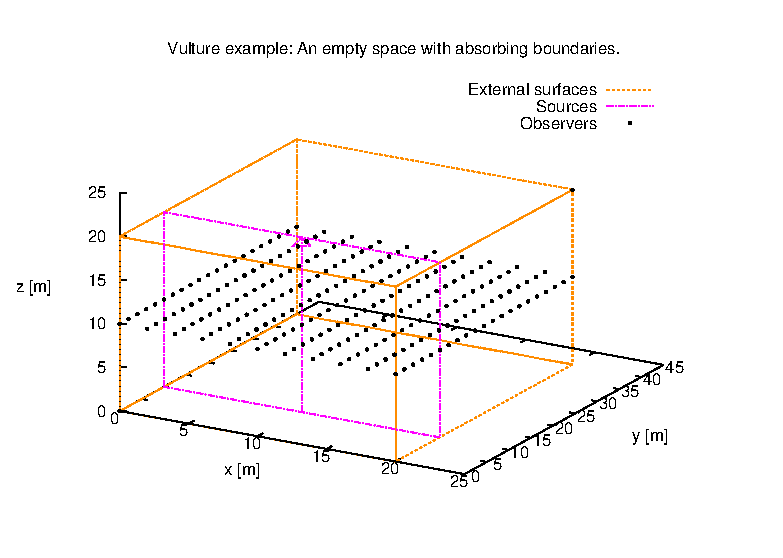
\includegraphics[width=14cm]{figures/free_space_mesh}}
\caption{\label{fg:free_space_mesh} Example 1 - Mesh geometry created by \texttt{gvulture} and \texttt{gnuplot}.}
\end{figure}

\begin{figure}[ht!]
 \centerline{\includegraphics[width=12cm]{figures/free_space_td}}
 \caption{\label{fg:free_space_td} Example 1 - Time response for $E_z$ at the centre of the mesh.}
 \centerline{\includegraphics[width=12cm]{figures/free_space_fd}}
 \caption{\label{fg:free_space_fd} Example 1 - Frequency response for $E_z$ at the centre of the mesh.}
\end{figure}

\subsubsection{Running the solver}

Now run the solver with the command
\begin{verbatim}
$ vulture -v free_space.mesh
\end{verbatim}
The progress of the simulation can be checked in the log file \texttt{vulture.log}, though
this example should run in only a few seconds.

\subsubsection{Viewing ASCII data}

The time response at the centre of the mesh from the ASCII observer will be
stored in the file \texttt{eh\_centre1\_td.dat}. This can be plotted with Gnuplot
using
\begin{verbatim}
set terminal post eps enhanced color 'Helvetica' 18
set output 'free_space_td.eps'
set xlabel 'Time (ns)'
set ylabel 'Electric field, E_z(10,20,10) (V/m)'
plot 'eh_centre1_td.asc' us ($2/1e-9):5 ti '' w l ls 1
\end{verbatim}
creating the image file \texttt{free\_space\_td.eps} shown in Figure \ref{fg:free_space_td}.

The response exhibits two interesting effects:
\begin{itemize}
 \item There is a non-physical DC response due to the charging of the grid capacitance associated
 with the discretised space. FDTD does not include explicit charge dynamics - charges only appear implicitly
 in the field distributions as determined by Gauss's Law. Hence,  since the Gaussian waveform has a DC component it displaces
 charge across the source plane leaving a net static field on the grid.  
 \item ``Spurious'' reflections from the edge of the mesh can be seen due to the truncation
 of the source plane. The source plane only has a finite size and hence the edge launches waves
 into the mesh.
\end{itemize}

The frequency spectrum at the centre of the mesh from the ASCII observer will be
stored in the file \texttt{eh\_centre2\_fd.dat}. This can be plotted with Gnuplot
using
\begin{verbatim}
set terminal post eps enhanced color 'Helvetica' 18
set output 'free_space_fd.eps'
se xlabel 'Frequency (MHz)'
se ylabel 'Electric field, |E_z|(10,20,10) (dB V/m)'
db20ri( r , i ) = 10.0 * log10 ( r**2 + i**2 )
plot 'eh_centre2_fd.asc' us ($1/1e6):(db20ri($6,$7)) ti '' w l lw 2
\end{verbatim}
creating the image file \texttt{free\_space\_fd.eps} shown in Figure \ref{fg:free_space_fd}.
The spurious DC response is
now isolated from the physical response. The ripples in the spectrum are
again a manifestation of the finite size of the source plane. In order to
increase the resolution of the spectrum the simulation needs to be run for
more time-steps.

\subsubsection{Post-processing binary data in the time-domain}

Edit the last line of the \texttt{process.dat} file created by the solver so that the file contains
\begin{verbatim}
CE  Vulture example: An empty space with absorbing boundaries.
1
 0 20 2 0 40 2 10 10 2
1 400
0 5.99585e+08 1.49896e+06
1
 10 10 20 20 10 10 3
\end{verbatim}
and then extract the time data at the centre of the mesh using
\begin{verbatim}
$ xtime
\end{verbatim}
which should create the output ASCII file \texttt{tdez.dat}.
This can be plotted with the previous ASCII data using the Gnuplot script
\begin{verbatim}
set terminal post eps enhanced color 'Helvetica' 18
set output 'free_space_td2.eps'
set xlabel 'Time (ns)'
set ylabel 'Electric field, E_z(10,20,10) (V/m)'
plot 'eh_centre1_td.asc' us ($2/1e-9):5 ti 'ASCII'  w l ls 1 , \
     'tdez.dat'          us 1:2         ti 'Binary' w l lw 2
\end{verbatim}
and should give identical results.

\subsubsection{Post-processing binary data in the frequency-domain}

The frequency response of all the data in the binary \texttt{impulse.dat}
file can be calculated using the command
\begin{verbatim}
$ xtransall phase
\end{verbatim}
where the \texttt{phase} argument requests that phase information is included - 
by default \texttt{xtransall} only generates magnitude information. Using the same \texttt{process.dat}
as in the previous section the command
\begin{verbatim}
$ xfreq phase
\end{verbatim}
will then extract the frequency response at the centre of the mesh into
the ASCII file \texttt{fdez.dat}. This can be plotted with
\begin{verbatim}
se xla 'Frequency (MHz)'
se yla 'Electric field, |E_z|(10,20,10) (dB V/m)'
plot 'fdez.dat' us 1:2 ti '' w l lw 2
se term post eps enhanced color 'Helvetica' 18
se ou 'um_eg1_plotfd.eps'
replot
\end{verbatim}
and again should be identical to the output from the ASCII observer.

\subsection{Example 2: An infinite parallel plate transmission line}

Another simple example is a parallel plate transmission line 
of ``infinite'' width. The top and bottom plates are represented using
PEC boundaries on the external surfaces of the mesh, while the infinite width of the
waveguide can by modelled by using PMC boundary conditions on 
the ``sides'' of the mesh. Compared to Example~1 we only need to change the 
boundary conditions on the external surfaces. The complete mesh file is 
\begin{verbatim}
VM 1.0.0
CE Vulture example: An empty parallel-plate waveguide.
# The mesh extents are 20x40x20 cells.
DM 20 40 20
GS
# Side walls are PMC.
BT XLO PMC
BT XHI PMC
# End walls are absorbing ABC.
BT YLO PML
BT YHI PML
# Top wals are PEC.
BT ZLO PEC
BT ZHI PEC
# The waveform is a Gaussian pulse with default paramters.
WF wf1 GAUSSIAN_PULSE
# The source is a surface of z-polarised soft electric fields.
EX  0 20 10 10  0 20 source EZ wf1 1.0
# Observe the fields on a plane, every second cell.
OP  0 20 0  40 10 10 plane TDOM_BINARY 2 2 2
# Observe the fields at the centre of the mesh.
OP 10 10 20 20 10 10 centre1 TDOM_ASCII
OP 10 10 20 20 10 10 centre2 FDOM_ASCII
GE
# Run for 400 time-steps.
NT 400 
# The mesh size is 1 m.
MS 1.0
EN
\end{verbatim}
and the output from \texttt{gvulture} looks exactly like the free-space example is 
Figure~\ref{fg:free_space_mesh}. We have also chosen to use PML absorbing 
boundaries on the open ends of the waveguide rather than the Mur ABCs used in Example~1.

\begin{figure}[ht!]
 \centerline{\includegraphics[width=12cm]{figures/parallel_plate_td}}
 \caption{\label{fg:parallel_plate_td} Example 2 - Time response for $E_z$ at the centre of the mesh.}
 \centerline{\includegraphics[width=12cm]{figures/parallel_plate_fd}}
 \caption{\label{fg:parallel_plate_fd} Example 2 - Frequency response for $E_z$ at the centre of the mesh.}
\end{figure}

The processing steps are exactly the same as for Example~1. The time response at the centre 
of the mesh is shown in Figure~\ref{fg:parallel_plate_td} and the frequency spectrum at the
smae point in Figure~\ref{fg:parallel_plate_td}. The ``spurious'' reflections from the edge of 
the mesh in the previous example 
have now disappeared since the source plane is now consistent with the boundary
conditions on the external surfaces of the mesh. The DC response has also disappeared
since the charge on the source plane edges can discharge into the PEC plates. A
soft electric field source can therefore excite an accutate TEM wave in a parallel-plate
waveguide structure, however, it launches a wave in both directions!

\begin{figure}[ht]
 \centerline{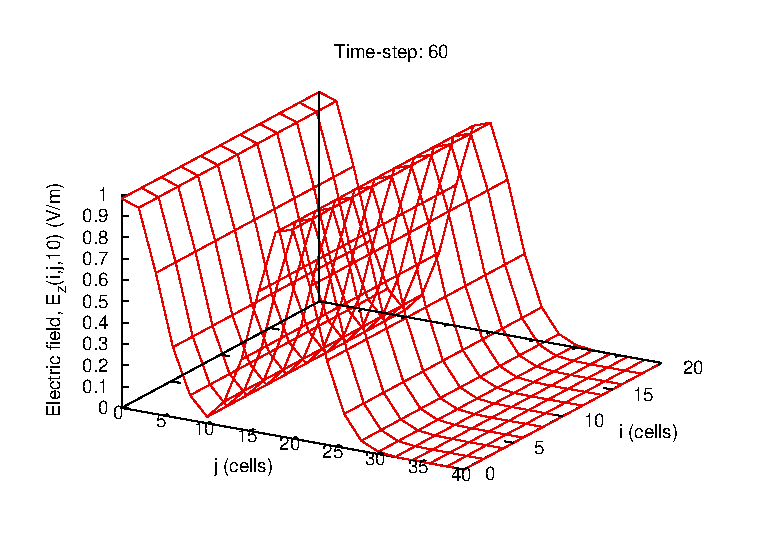
\includegraphics[width=12cm]{figures/parallel_plate_tds60}}
 \caption{\label{fg:parallel_plate_tds} Example 2 - Time response of $E_z$ across the $k=10$ plane at time-step 60.}
\end{figure}

The time response of the electric field can be extract from the binary observer
over a whole plane. To accomplish this for time-step number 60 modify the 
\texttt{process.dat} file to contain
\begin{verbatim}
CE  Vulture example: An empty parallel-plate waveguide.
1
 0 20 2 0 40 2 10 10 2
60 60
0 5.99585e+08 1.49896e+06
1
 0 20 0 40 10 10 3
\end{verbatim}
Here the parameters \texttt{n1} and \texttt{n2} are used to set the required output time-step
and the bounding box in the last line ranges over the whole observer plane.
Now run the \texttt{xplane} program
\begin{verbatim}
$ xplane
\end{verbatim}
This should generate an output file called \texttt{tdez.dat} containing mesh plot
data for the field that can be plotted using the Gnuplot script
\begin{verbatim}
set terminal post eps enhanced color 'Helvetica' 18
set output 'parallel_plate_tds60.eps'
set xlabel 'i (cells)'
set ylabel 'j (cells)'
set zlabel 'Electric field, E_z(i,j,10) (V/m)' rotate by 90 offset -1.5,1.5
set ticslevel 0
set title "Time-step: 60"
set view 120,60
splot 'tdez.dat' us 1:2:4 ti '' w l ls 1
\end{verbatim}
The result is shown in Figure~\ref{fg:parallel_plate_tds}. Note how the soft field source
excites a wave of amplitude one in both directions normal to the surface over which it is 
imposed. The amplitude depends on the CFLN as can be investigated by adding a \texttt{CN}
directive, such as
\begin{verbatim}
CN 0.99
\end{verbatim}
to section 3 of the mesh file. As the CFLN is increased the amplitude of the TEM wave
launched is reduce and visa-vera. 

The presence of both forward and backwards waves may or
may not be a problem depending on the application. The use of a PML in the open ends of
the waveguide is advisable to provide low reflection of the backward travelling wave into the mesh. 

\subsection{Example 3: An accurate plane-wave in free-space}

To launch an accurate plane-wave in free-space a total-field scattered-field plane-wave
source can be used. Starting from the mesh of Example~1 again we replace the distributed
electric field source with a plane-wave source and also change the external surfaces
to be PMLs rather than Mur ABCs. The complete mesh is now
\begin{verbatim}
VM 1.0.0
CE Vulture example: Plane wave in free-space.
# The mesh extents are 20x40x20 cells.
DM 20 40 20
GS
# Define all external surfaces to be PML.
BT XLO PML
BT XHI PML
BT YLO PML
BT YHI PML
BT ZLO PML
BT ZHI PML
# The waveform is a Gaussian pulse with default paramters.
WF wf1 GAUSSIAN_PULSE
# Plane-wave in +ve y direction, Ez polarisation.
PW  3 17  3  37  3 17 pw1 wf1 90 90 90 111111 1.0 0.0
# Observe the fields on a plane, every cell.
OP  0 20 0  40 10 10 plane TDOM_BINARY 1 1 1
# Observe the fields at the centre of the mesh.
OP 10 10 20 20 10 10 centre1 TDOM_ASCII
OP 10 10 20 20 10 10 centre2 FDOM_ASCII
GE
# Run for 400 time-steps.
NT 400 
# The mesh size is 1 m.
MS 1.0
EN
\end{verbatim}
The mesh now looks like Figure~\ref{fg:planewave_mesh}. The TFSF surface is shown as a box on the mesh
with arrows at the corner where the plane-wave first enters the total-field zone depicting the direction
of propagation (open arrow), polarisation direction the electric field (closed arrow) and polarisation
direction of the magnetic field (double open arrow). A higher density of observation points have been 
requested by changing the stride lengths in the binary observer to one cell.

\begin{figure}[ht]
\centerline{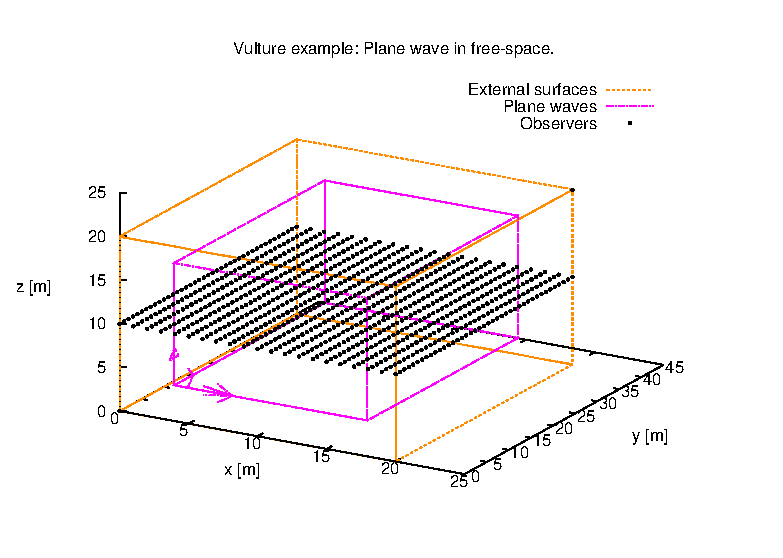
\includegraphics[width=12cm]{figures/planewave_mesh}}
\caption{\label{fg:planewave_mesh} Example 3 - Mesh geometry created by \texttt{gvulture} and \texttt{gnuplot}.}
\end{figure}

\begin{figure}[ht!]
 \centerline{\includegraphics[width=12cm]{figures/planewave_td}}
 \caption{\label{fg:planewave_td} Example 3 - Time response for $E_z$ at the centre of the mesh.}
 \centerline{\includegraphics[width=12cm]{figures/planewave_fd}}
 \caption{\label{fg:planewave_fd} Example 3 - Frequency response for $E_z$ at the centre of the mesh.}
\end{figure}

Proceeding with the same proccessing steps as before we obtain the time response and frequency spectrum at the
centre of the mesh shown in Figures~\ref{fg:planewave_td} and~\ref{fg:planewave_fd} respectively. Compared to Example~1 we
observe that a substantially improved plane-wave is excited within the total-field zone in the mesh. Up to a 
frequency corresponding to a mesh-size of one-tenth of a wavelength the amplitude of the wave remains within
0.1\,dB of the ideal value.

\begin{figure}[ht!]
\begin{center}
 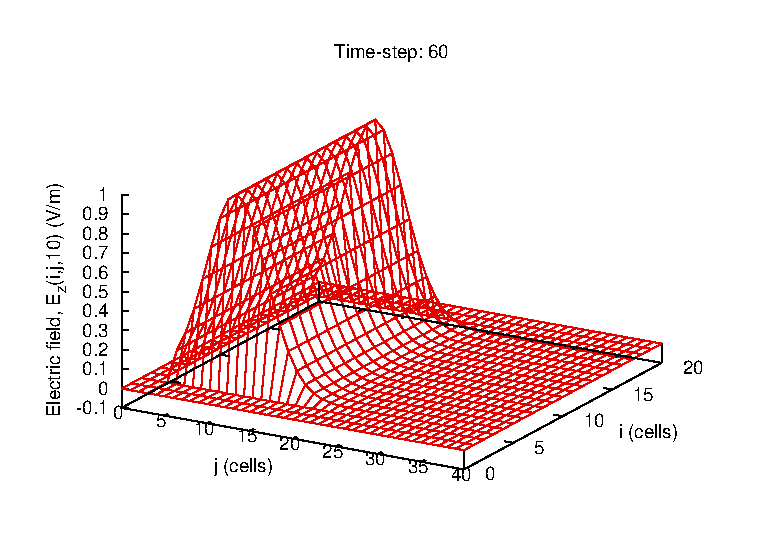
\includegraphics[width=0.49\linewidth]{figures/planewave_tds60}
 \includegraphics[width=0.49\linewidth]{figures/planewave_tds100}
 \caption{\label{fg:planewave_tds} Example 3 - Time responses of $E_z$ across the $k=10$ plane at time-steps 60 and 100.}
\end{center}
\end{figure}

Surface plots of the electric field over the plane of the binary observer can be obtained as before. For example
to get the response at time-step 60 modify the \texttt{process.dat} file to be
\begin{verbatim}
CE  Vulture example: Plane wave in free-space.
1
 0 20 1 0 40 1 10 10 1
60 60
0 5.99585e+08 1.49896e+06
1
 0 20 0 40 10 10 3
\end{verbatim}
and run 
\begin{verbatim}
$ xplane
\end{verbatim}
Figure~\ref{fg:planewave_tds} shows surface plots for time-steps 60 and 100. Notice how there is no field in the
scattered field zone since there are no scattering objects inside the TFSF surface. The plane-wave is completely
``reabsorbed'' by the TFSF surface at $j=37$.

An animation of the whole time response in the plane can be created by changing the time-step intervals in the
\texttt{process.dat} file to cover the whole time range:
\begin{verbatim}
CE  Vulture example: Plane wave in free-space.
1
 0 20 1 0 40 1 10 10 1
1 400
0 5.99585e+08 1.49896e+06
1
 0 20 0 40 10 10 3
\end{verbatim}
Using the command
\begin{verbatim}
$ mxplane
\end{verbatim}
a series of 400 data files with names \texttt{tds<nnn>.dat} are created that can be viewed in sequence to 
create an animation.
\begin{verbatim}
$ gnuplot
gnuplot> load 'plot'
\end{verbatim}

\subsection{Example 4: Transmission and reflection from a dielectric slab}

\begin{figure}[ht!]
  \centerline{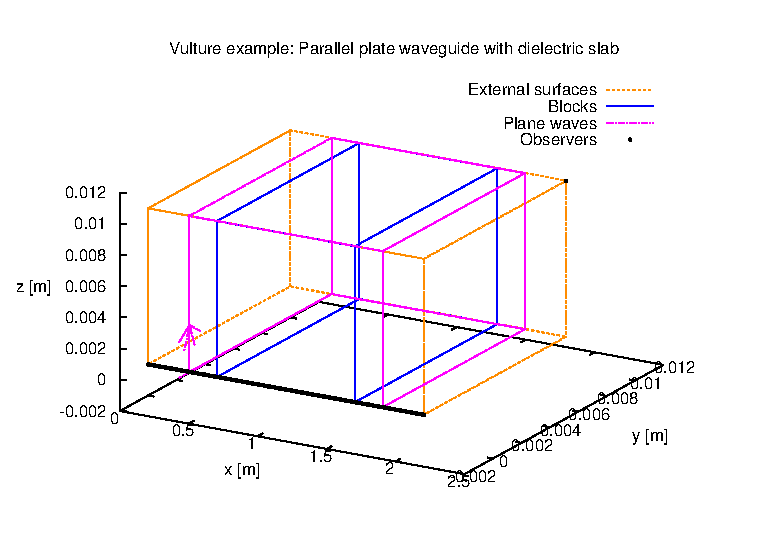
\includegraphics[width=12cm]{figures/parplate1D_dielslab_mesh}}
  \caption{\label{fg:parplate1D_dielslab_mesh} Example 4 - Mesh geometry created by \texttt{gvulture} and \texttt{gnuplot}.}
\end{figure}

This example calculates the reflection and transmission coefficient of an infinite dielectric slab to a normally
incident TEM wave. To simulate the infinite extent of the slab it is placed in the cross-section of 
a parallel-plate waveguide as was used in Example~2. Since the problem is invariant along the directions parallel 
to the plane of the slab only one cell needs to be used in those directions. The 
effectively one-dimensional mesh is given by
\begin{verbatim}
VM 1.0.0
CE Vulture example: Parallel plate waveguide with dielectric slab
DM 200   1   1
GS
# Parallel-plate waveguide boundary conditions.
BT XLO PML
BT XHI PML
BT YLO PEC
BT YHI PEC
BT ZLO PMC
BT ZHI PMC
# Simple dielectric medium.
MT dielectric SIMPLE 2.0 0.01 1.0
MB  50 150   0   1   0   1 dielectric
# Gaussian source.
WF wf1 GAUSSIAN_PULSE
# Partial TF/SF.
PW  30 170   0   1   0   1 pw1 wf1 90 0 180 110000 1.0 0.0
# Observe field reflected field if SF zone.
OP  20  20   0   0   0   0 ref1 TDOM_ASCII
OP  20  20   0   0   0   0 ref2 FDOM_ASCII
# Observe transmitted field in TF zone.
OP 160 160   0   0   0   0 trans1 TDOM_ASCII
OP 160 160   0   0   0   0 trans2 FDOM_ASCII
# Observe field along waveguide.
OP   0 200   0   0   0   0 line TDOM_BINARY 1 1 1
GE
NT 5000
MS 0.01
EN
\end{verbatim}
The lossy dielectric has a relative permittivity of 2 and a conductivity of 10\,mS/m. These
parameters are defined by the \texttt{MT} directive. The material parameters are applied to the mesh
between $i=50$ and $i=150$ by the \texttt{MB} directive. A TEM wave could be excited using
a plane of soft electric field sources as was done in Example~2. However, in this case we
use a partial TFSF plane-wave source, which has the advantage of allowing the reflected 
wave to be observed directly in the scattered field zone.

The mesh geometry is shown in Figure~\ref{fg:parplate1D_dielslab_mesh}. Only the \texttt{XLO} and \texttt{XHI} 
surfaces of the TFSF are active, as set by the mask \texttt{110000} in the \texttt{PW} directive. 
The wave is excited at $i=30$ and the upper surface of the TF-SF boundary is at $i=170$.  
Therefore the transmitted wave can be observed at the point $i=160$ in the total field zone 
and the reflected wave at $i=20$ in the scattered field zone. 

\begin{figure}[ht!]
\begin{center}
  \includegraphics[width=0.49\linewidth]{figures/parplate1D_dielslab-frame000050}
  \includegraphics[width=0.49\linewidth]{figures/parplate1D_dielslab-frame000100}
  \includegraphics[width=0.49\linewidth]{figures/parplate1D_dielslab-frame000150}
  \includegraphics[width=0.49\linewidth]{figures/parplate1D_dielslab-frame000200}
  \includegraphics[width=0.49\linewidth]{figures/parplate1D_dielslab-frame000250}
  \includegraphics[width=0.49\linewidth]{figures/parplate1D_dielslab-frame000350}
  \caption{\label{fg:parplate1D_dielslab_td} Example 4 - Time response at time-steps 50, 100, 150 and 350.} 
\end{center}
\end{figure}

\begin{figure}[ht!]
  \centerline{\includegraphics[width=12cm]{figures/parplate1D_dielslab_Smag}}
  \centerline{\includegraphics[width=12cm]{figures/parplate1D_dielslab_Sarg}}
  \caption{\label{fg:parplate1D_dielslab_fd} Example 4 - Scattering parameters of the dielctric slab: Magntitude (top) and phase (bottom).
  The phase reponse is only shown to 2\,GHz for clarity.}
\end{figure}

The solver is run in the usual way and the response along the length of the waveguide from the
binary observer is extracted at all time steps by editing the \texttt{process.dat} to read
\begin{verbatim}
CE  Vulture example: Parallel plate waveguide with dielectric slab
1
 0 200 1 0 0 1 0 0 1
1 1000
0 5.99585e+10 1.19917e+07
0.01
 0 200 0 0 0 0 2
\end{verbatim}
and then running
\begin{verbatim}
$ mxplane
\end{verbatim}
to obtain data files \texttt{tds<nnn>.dat} for the response along a line at each time-step. These can be
plotted using, for example, the Gnuplot script
\begin{verbatim}
set terminal post eps enhanced color 'Helvetica' 16
set output 'frame100.eps'
set style data lines 
set xrange [0:200]
set yrange [-1:1]
set xlabel 'x (cells)'
set ylabel 'E_y (V/m)'
set title 'time-step: 100'
set arrow 1 from  30,-1 to  30,1 nohead lt 0
set arrow 2 from 170,-1 to 170,1 nohead lt 0
set label 1 'SF' at  26,-0.9 left rotate by 90
set label 2 'TF' at  34,-0.9 left rotate by 90
set label 3 'TF' at 166,-0.9 left rotate by 90
set label 4 'SF' at 174,-0.9 left rotate by 90
set arrow 3 from  50,-1 to  50,1 nohead lt 0
set arrow 4 from 150,-1 to 150,1 nohead lt 0
set label 5 'Free-space' at  46,-0.9 left rotate by 90
set label 6 'Dielectric' at  54,-0.9 left rotate by 90
set label 7 'Dielectric' at 146,-0.9 left rotate by 90
set label 8 'Free-space' at 154,-0.9 left rotate by 90
plot 'tds100.dat' us 1:2 ti ''
\end{verbatim}

Figure \ref{fg:parplate1D_dielslab_td} shows the spatial variation of the field at a series of time-steps.
At time-step 50 the pulse is emerging from the lower TFSF boundary
and is approaching the dielectric's surface. By time-step 100 the pulse is approximately centred on the lower dielectric
interface and the reflected pulse is just becoming visible. At time-step 150 the reflected pulse has propagated away 
into the lower scattered-field zone and the transmitted pulse has cleared the dielectric interface and propagates 
into the medium. The attenuation of the pulse due to the dielectric loss can be observed at time-steps 200 and 250.
At time-step 350 the {\em incident field} has entered the upper scattered-field zone. Note, if there were no dielectric
present this field would be cancelled by the field which propagates through the total-field zone, giving zero scattered field.
However, the dielectric slab attenuates and delays the wave in the total-field zone and so a non-zero scattered field is 
manifested in the upper scattered-field zone.

The scattering parameters of the slab with reference to its surfaces are:
\begin{eqnarray}
S_{11} &=& \frac{E^-_z(50)}{E^+_z(50)} \\
S_{21} &=& \frac{E^+_z(150)}{E^+_z(50)}.
\end{eqnarray}
These can be calculated analytically~\cite{Orfanidis2010}. The fields at the slab surfaces are related to those at the observation and excitation points by
\begin{eqnarray}
\frac{E^+_z(160)}{E^+_z(150)} &=& \re^{ -\jmath \omega \cdot 10 \Delta t / c_0} \\
\frac{E^+_z(50)}{E^+_z(29)} &=& \re^{ -\jmath \omega \cdot 21 \Delta t / c_0} \\
\frac{E^-_z(20)}{E^-_z(50)} &=& \re^{ -\jmath \omega \cdot 30 \Delta t / c_0}
\end{eqnarray}
Note that in terms of the phase reference the plane-wave is effectively launched from one cell inside the
scattered field zone, hence the field $E^+_z(29)$ is used as the reference for the FDTD spectra. It
is usually more reliable to calibrate the incident field at the location of the front face of the 
dielectric by running a reference simulation with the dielectric slab removed and an observation
point at $i=50$ rather than relying on knowledge on the internal implementation of the code. Using the above we find that
\begin{eqnarray}
S_{11} &=& \re^{ \jmath \omega \cdot 51 \Delta t / c_0} \frac{E^-_r(20)}{E^+_z(29)} \\
S_{21} &=& \re^{ \jmath \omega \cdot 31 \Delta t / c_0} \frac{E^+_z(160)}{E^+_z(29)}.
\end{eqnarray}

Figure \ref{fg:parplate1D_dielslab_fd} shows the scattering parmeters of the dielectric slab compared with the analytical solution. 
It can be seen that the lower frequencies give accurate results whereas the higher frequency 
results are not so reliable. For high accuracy simulations the standard $\lambda/10$ rule of thumb is not
sufficient and a maximum mesh edge length of $\lambda/20$ should not be exceeded at the highest frequency of 
interest. In the analytic result a slab thickness of 101 cells was used - one more than
the thickness of the FDTD bounding box. This is because the simulation was run using an executable without
the averaged media support enabled and hence the dielectric material parameters are applied ``in-full'' on 
both the front and back (\texttt{XLO} and \texttt{XHI}) surfaces of the slab. Applied in this way the 
material parameters are effective to about half a cell from these surfaces leading to an overall
effective thickness one cell greater than the bounding box thickness.

\subsection{Example 5: Transmission and reflection from a thin boundary}

\subsection{Example 6: Radiation from an infinitesimal Hertzian dipole}

\subsection{Example 7: Radiation from a half-wave dipole}

\subsection{Example 8: Plane-wave penetration through an aperture}

This example looks at the transmission through a small square aperture in an infinite PEC plate using
a truncated plane-wave excitation. The mesh for the problem is:
\begin{verbatim}
VM 1.0.0
CE Vulture example: Aperture in infinite plane
DM 60 40 40
GS
# Free-space boundaries.
BT XLO PML
BT XHI PML
BT YLO PML
BT YHI PML
BT ZLO PML
BT ZHI PML
# Solid PEC sheet
#TB 30 30  0 40  0 40 PEC
# PEC sheet with 2x2 cell square aperure.
# TB 30 30  0 40  0 19 PEC
# TB 30 30  0 40 21 40 PEC
# TB 30 30  0 19 19 21 PEC
# TB 30 30 21 40 19 21 PEC
# Differentiated Gaussian pulse waveform
WF wf1 DIFF_GAUSSIAN_PULSE 1.0
# Full plane-wave for empty mesh case.
PW  5 55  5 35  5 35 pw1 wf1 90.0   0.0  90.0 111111 1.0 0.0
# Truncated incident wave.
PW  5 30  5 35  5 35 pw1 wf1 90.0   0.0  90.0 101111 1.0 0.0
# Add reflected wave using second plane-wave, delay by flight time along bbox.
# PW  5 30  5 35  5 35 pw2 wf1 90.0 180.0 270.0 101111 1.0 8.339e-11
# Magnetic moment source using differential waveform
# dt = 1.667818e-12
# dl = 1e-3
# a = 2 * dl
# alpha = 4 * a^3 / 3 / pi^1.5
# Hsc = 2 / eta0
# m = -alpha * Hsc
# sigma = 5 * sqrt(2) * dt
# Imdl = mu0 * m * 1 / sigma * d/dt WF
# delay = ( 25 + 0.5 ) * dl / c0 
# WF wf2 RICKER_WAVELET 1.0
# EX 30 31 19 19 19 21 dipmom IMDY wf2 1.0836e-06 8.5059e-11
# Observe incident field point.
OP 29 29 20 20 20 20 inc1 TDOM_ASCII
OP 29 29 20 20 20 20 inc2 FDOM_ASCII
# Observe transmitted field on axis of aperture.
OP 50 50 20 20 20 20 trans1 TDOM_ASCII
OP 50 50 20 20 20 20 trans2 FDOM_ASCII
# Observe fields in plane through aperture.
OP  0 60  0 40 20 20 plane TDOM_BINARY 1 1 1 
GE 
NT 200
MS 0.001
EN
\end{verbatim}
Some parts of the mesh are commented out and will be used later. The active parts currently simulate a 
plane-wave in free space to use as a reference case. The simulation is run and the data post-processed using
the same steps as in the previous examples. The tangential magnetic field spectrum at mesh point $(29,20,20)$ 
is shown in Figure~\ref{fg:aperture-incident} and as expected it has a uniform magnitude of $1/\eta_0$\,A/m.

\begin{figure}[ht]
 \centerline{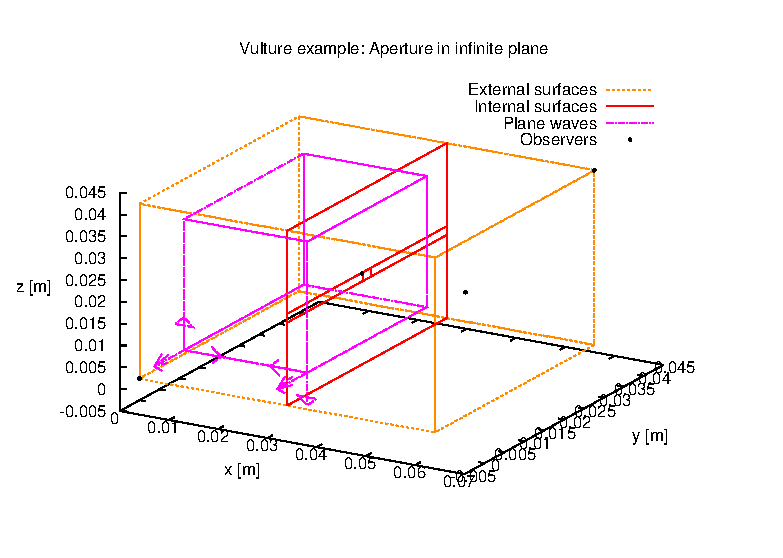
\includegraphics[width=0.80\linewidth]{figures/aperture-mesh}}
 \caption{\label{fg:aperture-mesh} Example 8 - Geometry of the aperture transmission problem, showing
 the TFSF bounding box, aperture and observation points either side of the aperture plane. The plane observer
 points are not shown for clarity.}
\end{figure}

\begin{figure}[ht!]
 \includegraphics[width=0.49\linewidth]{figures/aperture-solid-frame000120}
 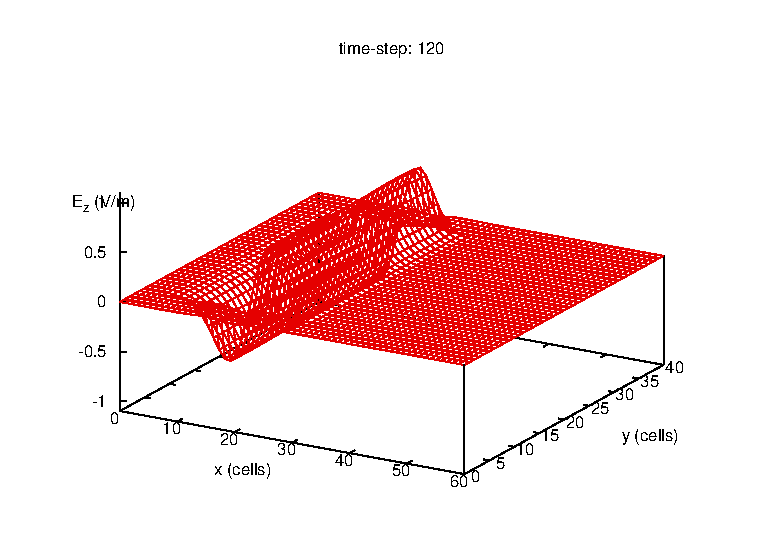
\includegraphics[width=0.49\linewidth]{figures/aperture-solidreflect-frame000120}
 \centerline{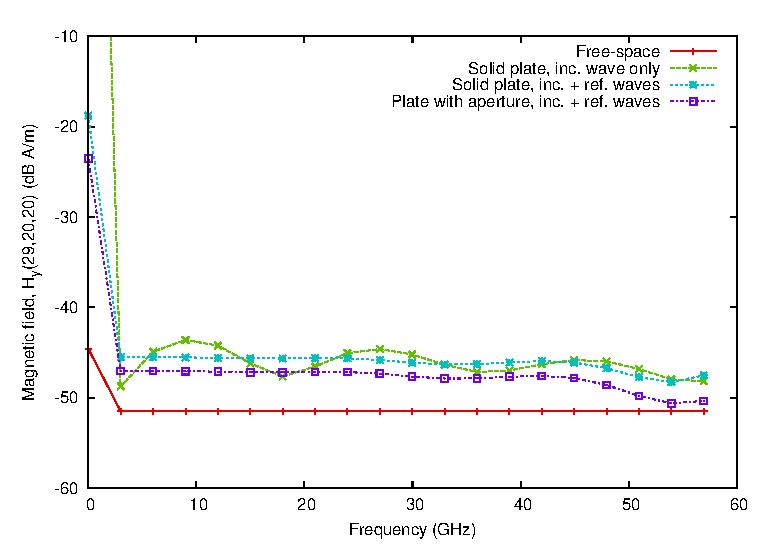
\includegraphics[width=0.80\linewidth]{figures/aperture-Hsc}} 
 \caption{\label{fg:aperture-incident} Example 8 - Spatial response of electric across a plane for a plane-wave incident on a
 solid PEC plate at time step 120 without (top left) and with (top right) the reflected wave 
 included in the TF-SF exciation. The frequency reponse of the tangential magnetic field directly next to the
 PEC plane is shown below.}
\end{figure}

Now the problem space is cut by introducing a solid PEC surface in the $i=30$ plane
\begin{verbatim}
# Solid PEC sheet
TB 30 30  0 40  0 40 PEC
...
\end{verbatim}
and replacing the full TFSF surface by a partial surface
\begin{verbatim}
...
# Truncated incident wave.
PW  5 30  5 35  5 35 pw1 wf1 90.0   0.0  90.0 101111 1.0 0.0
...
\end{verbatim}
which only extends as far as the PEC plate and where the \texttt{XHI} surface has been deactivated 
using the mask \texttt{101111}. The wave at time-step 120, after the wave has reflected from the PEC surface,
is shown in the top-left of Figure~\ref{fg:aperture-incident}. It can be seen that it is quite distorted compared to
the expected superposition of incident and reflected plane-waves. This is because the TFSF surface only
injects the incident field into the total field region and the reflected field ``spills out'' into the
scattered field region. The effect can also be seen in the amplitude spectrum of the tangential magnetic 
field at the PEC surface, which exhibits some ripples compared to the expected flat value of $2/\eta_0$.
This can be thought of as arising from secondary Huygen's sources located along the edges
where the TFSF and PEC plate intersect; on these edge the field injected by the TFSF surface does not satisfy the
PEC boundary conditions. To remedy this the reflected wave can be included in the field injected by the TFSF surface.
In Vulture this can be accomplished by adding a second \texttt{PW} directive with a wave travelling in the opposite direction, with
the opposite polarisation:
\begin{verbatim}
...
# Add reflected wave using second plane-wave, delay by flight time along bbox.
PW  5 30  5 35  5 35 pw2 wf1 90.0 180.0 270.0 101111 1.0 8.339e-11
...
\end{verbatim}
The wave is also delayed by a time of $(30-5)\Delta /\mathrm{c}_0=8.339$\,ps, corresponding to the propagation time along the
partial Huygen's surface, so the reflected wave begins as the incident wave strikes
the PEC plate. The wave at time-step 120 with this reflected wave included is shown in the top-right 
of Figure~\ref{fg:aperture-incident}. This shows a substantial improvement in the wave shape. There is still some
distortion due to the fact that the incident wave undergoes dispersion as it propagates towards the PEC
plate that is not accounted for by the injected reflected wave. In a ``real'' simulation the length of the TFSF
box would be reduced to one or two cells as in
\begin{verbatim}
...
# Add reflected wave using second plane-wave, delay by flight time along bbox.
PW 28 30  5 35  5 35 pw2 wf1 90.0 180.0 270.0 101111 1.0 8.339e-11
# Truncated incident wave.
PW 28 30  5 35  5 35 pw1 wf1 90.0   0.0  90.0 101111 1.0 0.0
...
\end{verbatim}
in order to mitigate these dispersion effect. Here, for the sake of presentation, the TFSF has been
made sufficiently long to allow the incident and reflected waves to be seen clearly. 

Now that we have an accurate incident field, a small square aperture of side length $a=2\Delta l$ is cut 
in the PEC plate by replacing the solid plate \texttt{TB} directive with
\begin{verbatim}
...
# PEC sheet with 2x2 cell square aperure.
TB 30 30  0 40  0 19 PEC
TB 30 30  0 40 21 40 PEC
TB 30 30  0 19 19 21 PEC
TB 30 30 21 40 19 21 PEC
...
\end{verbatim}
The mesh for this case is shown in Figure~\ref{fg:aperture-mesh}. The transmitted wave is shown in the
top-left of Figure~\ref{fg:aperture-radiation} at time-step 130. A ``spherical'' wave can be seen radiating from
the aperture. The transmitted electric field is observed at mesh cell $(50,20,20)$ and its time series 
is shown in the graph in the lower part of Figure~\ref{fg:aperture-radiation}.

\begin{figure}[ht!]
 \includegraphics[width=0.49\linewidth]{figures/aperture-frame000130}
 \includegraphics[width=0.49\linewidth]{figures/aperture-equivdipole-frame000130}
 \centerline{\includegraphics[width=0.80\linewidth]{figures/aperture-Erad}} 
 \caption{\label{fg:aperture-radiation} Example 8 - Spatial response of the electric field transmitted by the aperture 
 across a plane at time-step 130 for the physical aperture (top left) and equivlanet dipole (top right).
 The time reponse of the electric field at a point on the axis of the aperture is shown below.}
\end{figure}

The field radiated by a small aperture can be approximated by the field from a set of equivalent dipole
moments~\cite{Chen1974}. For a normally incident plane-wave only the magnetic dipole moment polarised in the direction of the
magnetic field is excited and this is given by
\begin{eqnarray}
m_y = \alpha_{\mathrm{M};yy} H^\mathrm{SC}_y = 2 \alpha_{\mathrm{M};yy} H^\mathrm{inc}_y,
\end{eqnarray}
where $\alpha_{\mathrm{M};yy}$ is the magnetic polarisability of the aperture and $H^\mathrm{SC}_y$ is 
the short-circuited magnetic field on the incident field side, equal to twice the incident magnetic
field $H^\mathrm{inc}_y$~\cite{McDonald1987}. The polarisability of the aperture is approximately
\begin{eqnarray}
\alpha_{\mathrm{M};yy} = \frac{4 a^3}{3 \sqrt{\pi}^3},
\end{eqnarray}
where $a$ is the side length. The current moment of the equivalent infinitesimal magnetic dipole is
given by
\begin{eqnarray}
I_{\mathrm{M};y}(t) \dif{y} = \mu_0 \deriv{m_y}{t}
\end{eqnarray}
and from the above we can write this
\begin{eqnarray}
I_{\mathrm{M};y}(t) \dif{y} &=& \mu_0 \frac{8 a^3}{3 \sqrt{\pi}^3} \deriv{H^\mathrm{inc}_y}{t}.
\end{eqnarray}
In the ``real'' aperture similation the incident waveform was a differentiated Gaussian pulse, $\psi_\mathrm{DGP}(t)$, so
accounting for the delay between the waveform and the location of the equivalent dipole moment of the aperture is
\begin{eqnarray}
I_{\mathrm{M};y}(t) \dif{y} 
&=& \frac{\mu_0}{\eta_0} \frac{8 a^3}{3 \sqrt{\pi}^3} \left. \deriv{\psi_\mathrm{DGP}}{t} \right|_{t-25.5\Delta t}.
\end{eqnarray}
The derivative of the differentiated Gaussian pulse waveform is just a scaled version of the Ricker Wavelet
waveform so finally
\begin{eqnarray}
I_{\mathrm{M};y}(t) \dif{y}
&=& \frac{\mu_0}{\eta_0} \frac{8 a^3}{3 \sqrt{\pi}^3} \frac{1}{\sigma_\mathrm{GP}} \psi_\mathrm{RW}(t-25.5\Delta t).
\end{eqnarray}
This can be implemented in the simulation by removing the plane-wave source, closing the aperture in the PEC
plate and then introducing the magnetic moment source
\begin{verbatim}
...
# WF wf2 RICKER_WAVELET 1.0
EX 30 31 19 19 19 21 dipmom IMDY wf2 1.0836e-06 8.5059e-11
...
\end{verbatim}

The top-right part of Figure~\ref{fg:aperture-radiation} shows the wave radiated by this equivalent 
dipole moment source. While it is similar to that of the aperture it is not the same. Looking at
the wave at $(50,20,20)$ is can be seen that the wave from the equivalent dipole moment is larger 
and slightly ahead of that of the physical aperture simulation. The reasons for this are:
\begin{itemize}
 \item The effective size of the aperture on the discretised FDTD grid is smaller than $a=2\Delta l$.
 The PEC conditions are enforced on the aperture edges, but have an effective ``range of influnence'' of
 the order of $\Delta l/2$. The effective size of the aperture is there somewhat smaller than $2\Delta l$.
 \item The grid dispersion of the incident wave in the physical aperture simulation is not accounted for
 in the equivalent dipole simulation.
 \item The physical aperture may have some dispersion (delay) associated with its finite size.
\end{itemize}
Good agreement between the physical aperture simulation and equivalent dipole simulation can be obtained
using an effective aperture size of $a=1.49\Delta l$ and adding an excess delay of 7\,ps, as shown in
Figure~\ref{fg:aperture-radiation}. By varying the number of cells in the aperture while keeping the
physical aperture size fixed it can be shown that at least 8 cells per side are required to obtain
an accuracy of 12\,\% or better.

\subsection{Example 9: Shielding effectiveness of an enclosure with an aperture}

\begin{figure}[ht]
 \centerline{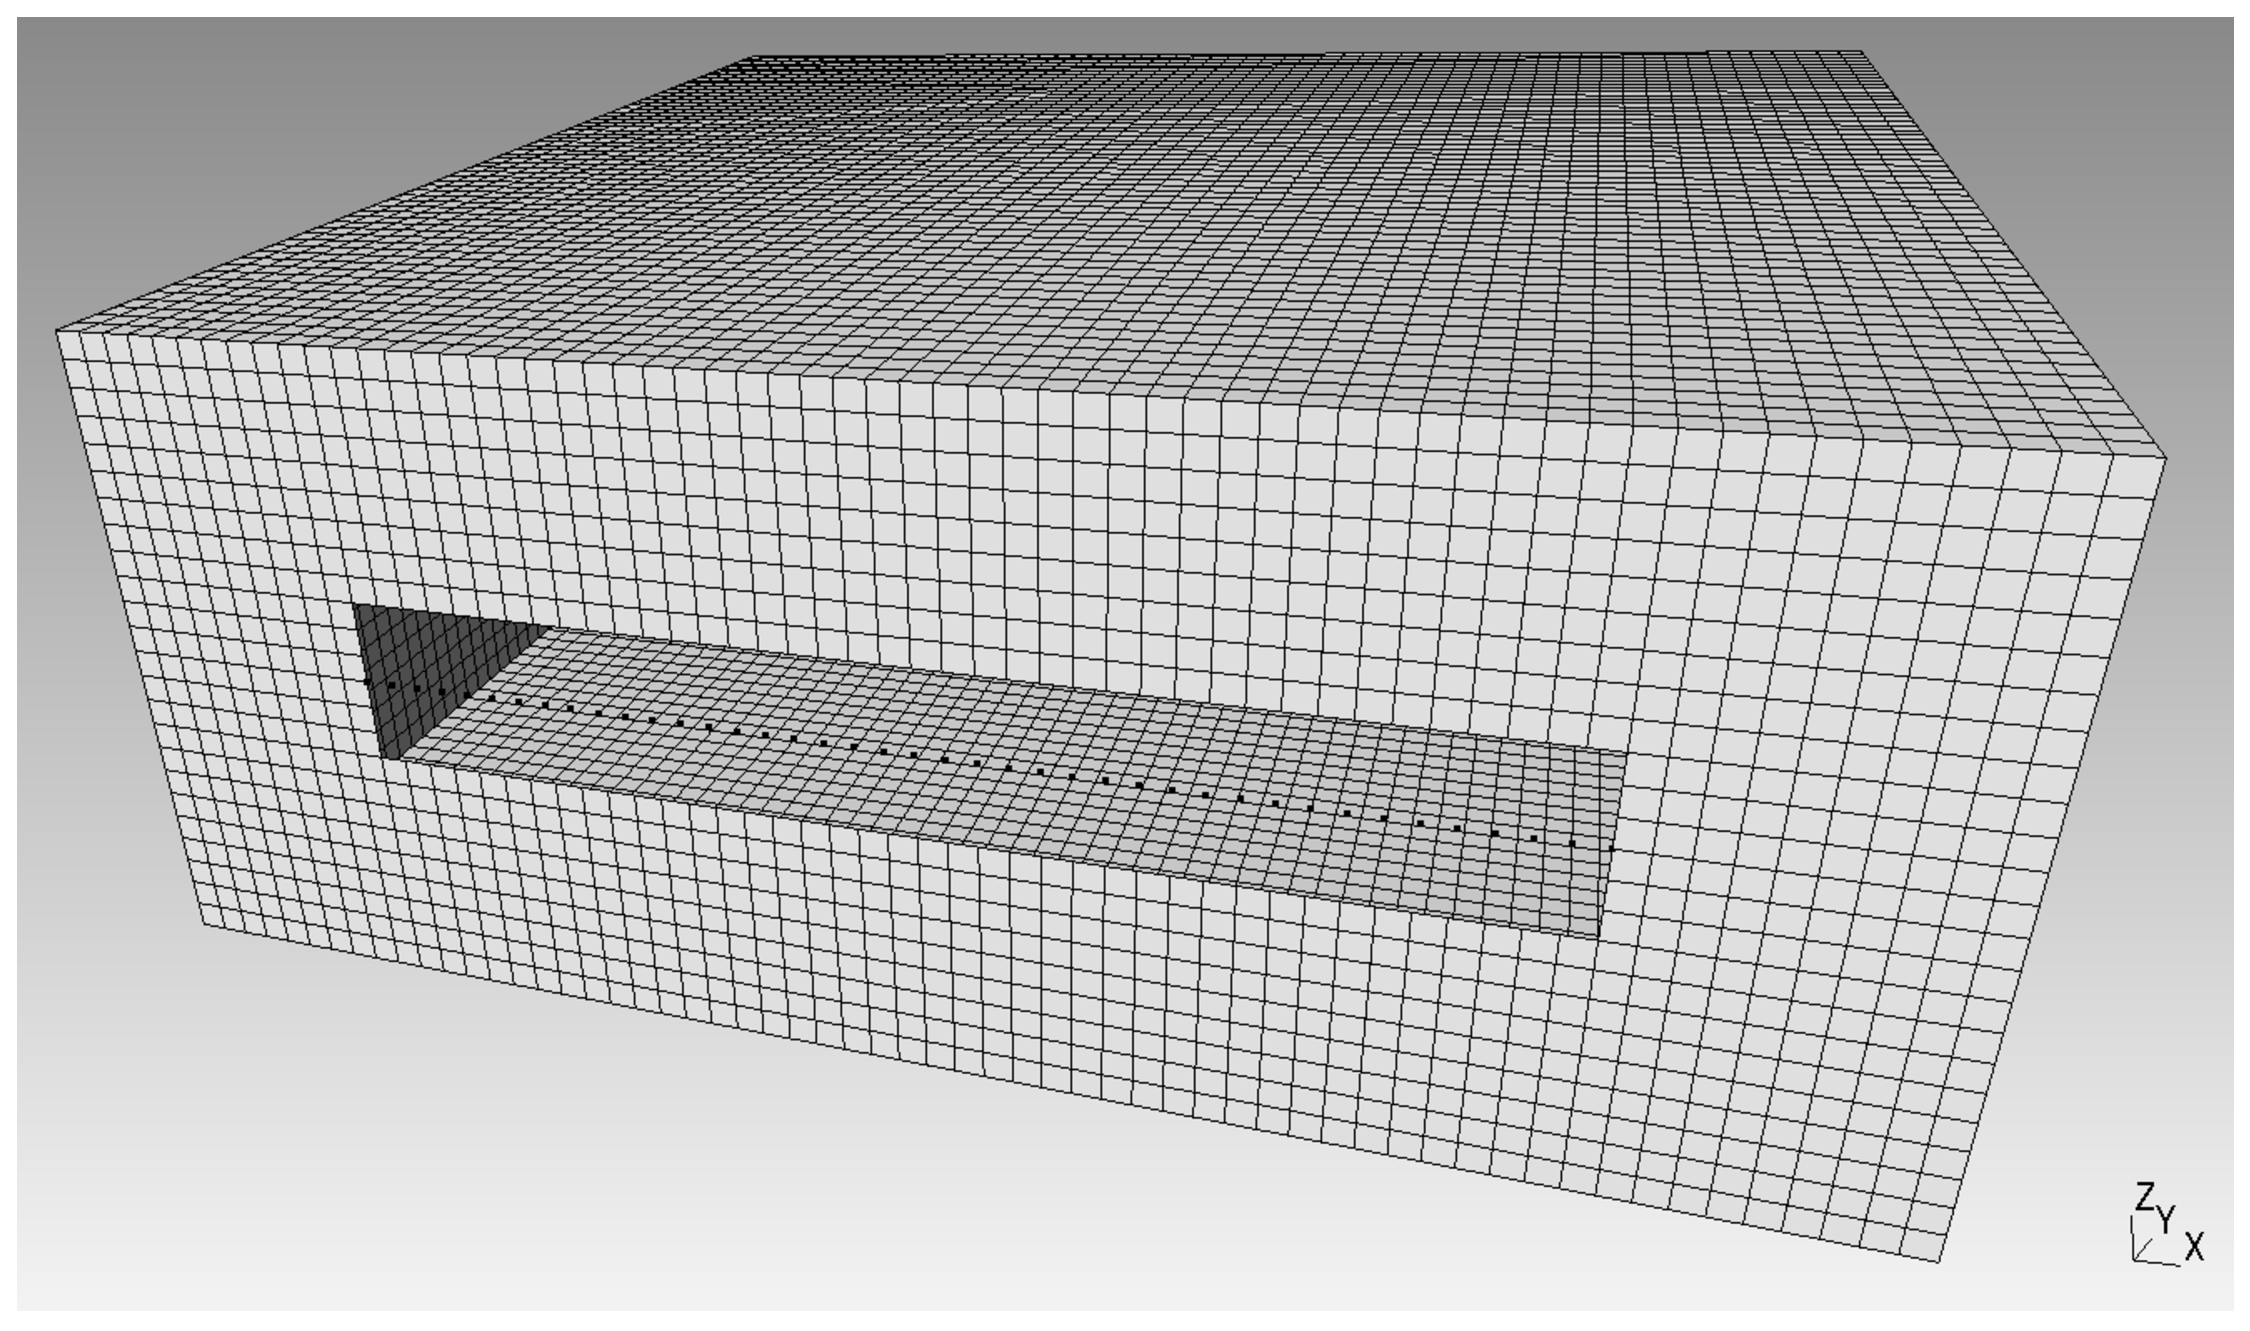
\includegraphics[width=12cm]{figures/enclosure_se-mesh}}
 \caption{\label{fg:enclosure_se-mesh} Example 9 - Mesh geometry created by \texttt{gvulture} and \texttt{gmsh}.}
\end{figure}

This example consists of a metal sided enclosure of dimensions $300\times 120\times 300$\,mm with a $200\times 30$\,mm slot in the centre of one
side. The enclosure is illuminated by a plane-wave which is normally incident on the slot. 
The input mesh file is:
\begin{verbatim}
VM 1.0.0
CE Vulture example: Enclosure with slot.
DM 80 100 44
GS
# Front face of enlcosure with slot..
TB 10 70 30 30 10 19 PEC
TB 10 70 30 30 25 34 PEC
TB 10 20 30 30 19 25 PEC
TB 60 70 30 30 19 25 PEC
# Back face.
TB 10 70 90 90 10 34 PEC
# Top face.
TB 10 70 30 90 34 34 PEC
# Bottom face.
TB 10 70 30 90 10 10 PEC
# Left face.
TB 10 10 30 90 10 34 PEC
# Right face.
TB 70 70 30 90 10 34 PEC
# Gaussian waveform.
WF wf1 GAUSSIAN_PULSE
# Incident plane-wave.
PW 15 65 10 30 14 30 pwinc wf1 90.0  90.0  90.0 111011 1.0 0.0
# Reflected plane-wave.
PW 15 65 10 30 14 30 pwref wf1 90.0 270.0 270.0 111011 1.0 3.3356e-10
# Observers at centre of top face.
OP 40 40 60 60 22 22 centre1 TDOM_ASCII
OP 40 40 60 60 22 22 centre2 FDOM_ASCII
# Observer for field in the slot.
OP 40 40 29 29 22 22 slot1 TDOM_ASCII
OP 40 40 29 29 22 22 slot2 FDOM_ASCII
GE
NT 80000
MS 5e-3
EN
\end{verbatim}
The enclosure is constructed from PEC surface materials. A partial TFSF is again used to introduce the plane-wave 
excitation of the slot and the reflected wave and we observe the fields in the slot and at the centre of the enclosure.
The geometry as viewed in Gmsh is shown in Figure \ref{fg:enclosure_se-mesh}. The Gmsh input file can be created using
\begin{verbatim}
$ gvulture -e -p -m enclsoure_se.mesh
\end{verbatim}
and then viewed in Gsmh with
\begin{verbatim}
$ gmsh mesh.msh
\end{verbatim}

\begin{figure}[ht!]
 \centerline{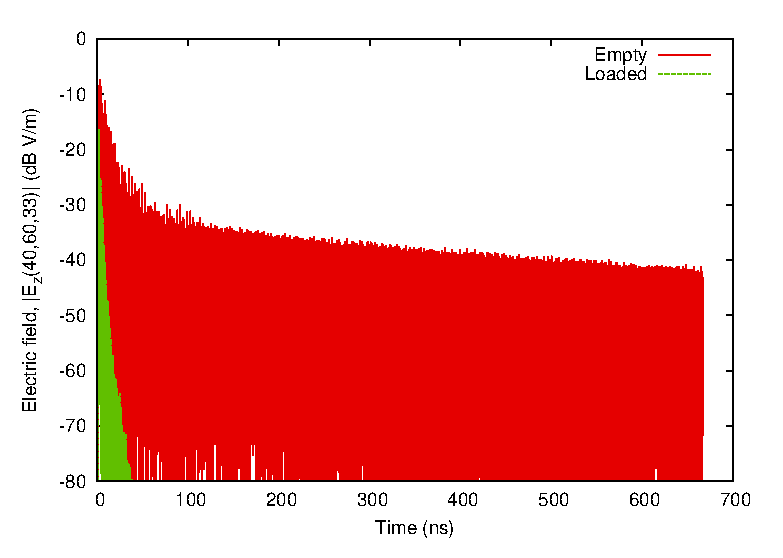
\includegraphics[width=12cm]{figures/enclosure_se_tdlog}}
 \caption{\label{fg:enclosure_se_td} Example 9 - Time response at centre of enclosure. The amplitude of the electric 
 field is plotted in decibels, showing the long exponential decay of the field inside the unloaded enclosure compared to
 the rapid decay when the enclosure is loaded with an LS22 block.}
 \centerline{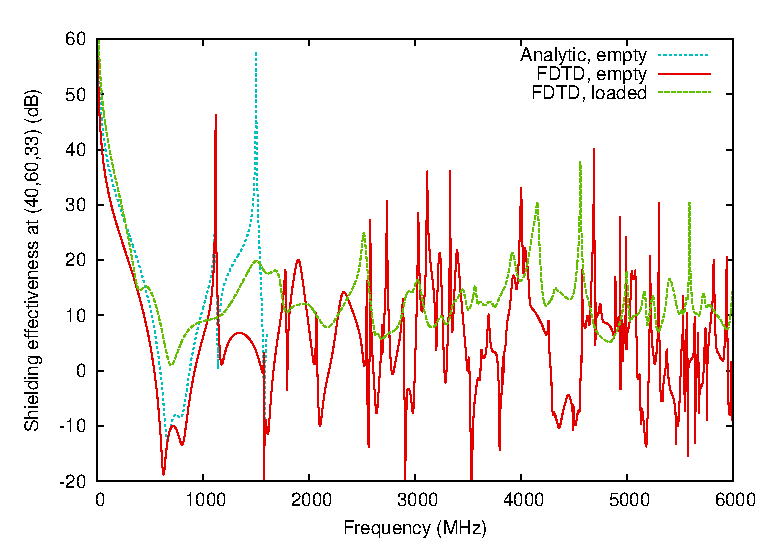
\includegraphics[width=12cm]{figures/enclosure_se_fd}}
 \caption{\label{fg:enclosure_se_fd} Example 9 - Shielding effectiveness at centre of enclosure with and without loading. The analytic model
 is only valid up to the first resonance of the enclosure.}
\end{figure}

The time response of the observation point at the centre of the enclosure is shown in 
Figure~\ref{fg:enclosure_se_td}. The attenuation of the signal is entirely due to re-radiation of energy
back through the slot since there are no other loss mechanisms inside the enclosure.
The shielding effectiveness of the enclosure can be defined as the amount by which the incident 
field is attenuated by the enclosure's presence. If the incident plane-wave field amplitude is $|E^\mathrm{inc}|$ and the internal
field amplitude is $|E^\mathrm{int}|$ then we can define
\begin{eqnarray}
S_\mathrm{E} = \frac{|E^\mathrm{inc}|}{|E^\mathrm{int}|}.
\end{eqnarray}
In order to obtain an accurate frequency spectrum from a time response a rule-of-thumb is that the time response
should have decayed by 60\,dB from its maximum value. The response in Figure~\ref{fg:enclosure_se_td} has only
decayed by about 35\,dB so a spectrum obtained from it should be treated with caution. 

Clearly the field inside the enclosure is highly non-uniform so the shielding effectiveness depends
on the position within the enclosure.  Figure \ref{fg:enclosure_se_fd} shows the shielding effectiveness
at the centre of the cavity, which since the incident field amplitude is unity is just the reciprocal of $|E_z(40,60,22)|$, 
compared to the prediction of a simple analytical model~\cite{Robinson1996}. The two results agree well up 
to just over 1\,GHz. Beyond this frequency the analytic model becomes invalid due to the excitation of higher order modes.

Once a cavity is loaded by contents the response will change. To respresent this effect we introduce a 100\,mm
sided cube of radio absorbing material into the enclsoure. The material is a commercially available absorber, 
Eccosorb LS22~\cite{eccosorb}. The material's complex permittivity, obtained from the manufacturer's data-sheet, is shown in figure~\ref{fg:ls22fit}
together the result of applying a genetic algorithm to fit the complex permittivity to a third order Debye dispersion
relationship. The Debye parameters obtained are given in Table~\ref{tb:ls22debye}.

\begin{table}[ht]
\begin{center}
\begin{tabular}{|c|c|c|c|c|}
\hline
$k$     &$\Delta \epsilon_k$ &$\tau_k$   &$r_k$           &$p_k$           \\
(-)     &(-)                 &           &(rad\,s$^{-1})$ &(rad\,s$^{-1})$ \\
\hline
1       &0.00109             &0.1\,s     &5.45118e-03     &-1.00000e+01    \\
2       &6.632               &0.1062\,ns &3.12249e+10     &-9.41658e+09    \\
3       &3.27                &15.781\,ps &1.03602e+11     &-6.33664e+10    \\
\hline
\end{tabular}
\caption{\label{tb:ls22debye}Example 9 - Debye model for LS22 RAM: $\epsilon_\infty=1$, $\sigma=0.344191$.}
\end{center}
\end{table}

\begin{figure}[ht!]
 \centerline{\includegraphics[width=10cm]{figures/LS22-3pole}}
 \caption{\label{fg:ls22fit} Example 9 - Complex permittivity of LS22 RAM comparing manufacturer's data to
 a third order Debye model obtained using a genetic algorithm.}
\end{figure}

The absorber is introduced to the mesh by adding the following two directives
\begin{verbatim}
MT ls22 DEBYE "LS22-3pole.prm"
MB 30 50 60 80 12 32 ls22
\end{verbatim}
The Debye parameters are then entered into an ASCII file called \texttt{LS22-3pole.prm}
which should contain:
\begin{verbatim}
3  1.00000e+00  3.44191e-01  1.00000e+00
 1.03602e+11  0.00000e+00 -6.33664e+10  0.00000e+00
 5.45118e-03  0.00000e+00 -1.00000e+01  0.00000e+00
 3.12249e+10  0.00000e+00 -9.41658e+09  0.00000e+00
\end{verbatim}

Running the simulation again we obtain the results denoted by ``Loaded'' in Figures~\ref{fg:enclosure_se_td} 
and ~\ref{fg:enclosure_se_fd}. The time response now decays much more quickly than that of the empty enclosure 
and the shielding effectiveness at the centre of the enclosure is generally increased by 20\,dB. The resonant 
features are smeared out and damped by the absorber, though some sharp features remain and there are frequencies
at which the shielding has decreased. 

TBC:
\begin{itemize}
 \item Decay time calculation and graph annotation.
 \item Required energy decay for reliable DFT.
 \item Partial Q-factor and decay rate of aperture.
 \item Partial Q-factor and decay rate of LS22.
\end{itemize}

\subsection{Example 10: Stripline and microstrip line parameters}

\begin{figure}[ht]
\centerline{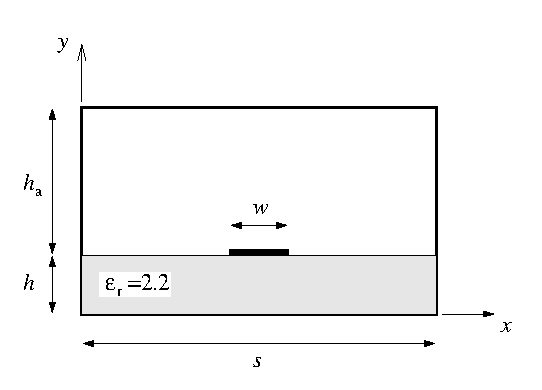
\includegraphics[width=0.4\linewidth]{figures/shielded_microstrip}}
\caption{\label{fg:shielded_microstrip}Cross-section of the shielded 
  microstrip line.}
\end{figure}

This example considers a shielded microstrip structure, as used by 
Gedney~\cite{Gedney1996a}, and shown in Figure~\ref{fg:shielded_microstrip}.  
The dimension of the structure are $w=0.254$\unit{mm}, $h=0.254$\unit{mm}, 
$h_\ra=0.762$\unit{mm}, $s=2.11$\unit{mm} and the permittivity 
is $\epsilon_\rr=2.2$. The structure is modelled on a grid with 
$\Delta l=0.042333\unit{mm}$ giving an overall grid of dimensions 
$50\times 24 \times 400$ and time step of $\Delta t=70.5555\unit{fs}$. 
The line was excited using a plane of $y$-polarised electric field points underneath the track at
the centre of the mesh in the $z$ direction. A broad Gaussian pulse
was used, with a bandwidth of 450\unit{GHz}. PML boundaries were used
to terminate the problem space at the lower and upper $z$ boundaries.
This structure therefore allows the near normal incidence reflection
the inhomogeneous PML to be studied.

\begin{figure}[ht]
\centerline{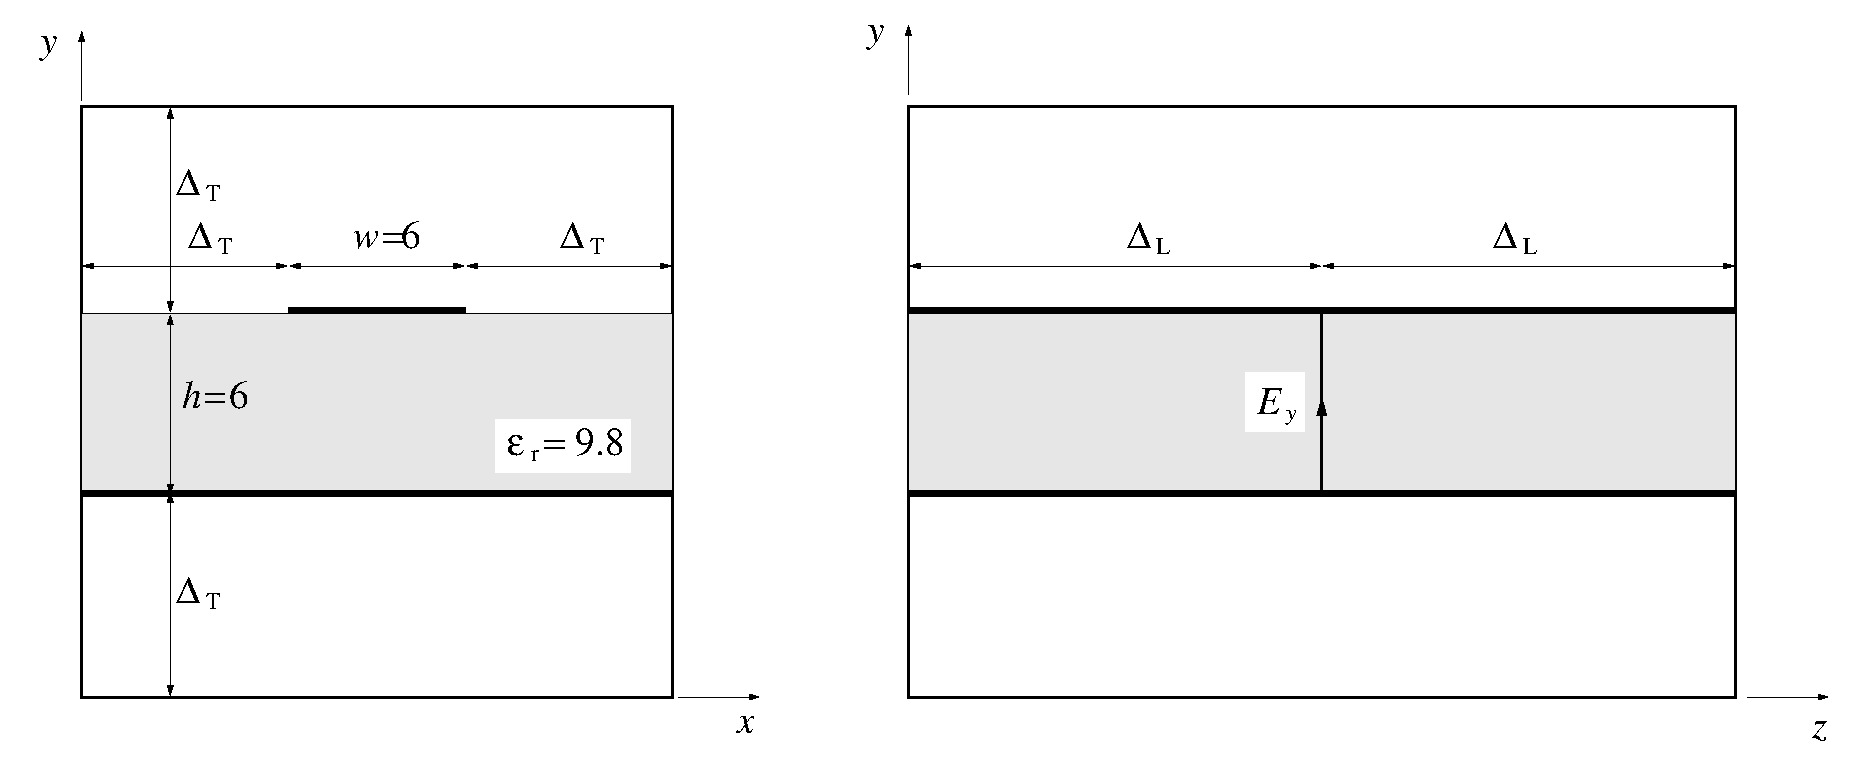
\includegraphics[width=0.75\linewidth]{figures/microstrip}}
\caption{\label{fg:microstrip}Cross-section of the microstrip line.}
\end{figure}

Replacing the PECs on the sides of the mesh with PML we obtain the open microstrip
structure shown in Figure~\ref{fg:microstrip}.

[TBD:  Determination of voltage, current, characterstic impedance, propagation constant 
and effective permittivity.]

%
% ----------------------------------------------------------------------- 
%    
% References
%
% ----------------------------------------------------------------------- 
%
%\nocite{*}
\bibliographystyle{ieeetr} 
\bibliography{References}
\label{sc:references}
\newpage
%
% ----------------------------------------------------------------------- 
%    
% Appendices
%
% ----------------------------------------------------------------------- 
%
\appendix
%
% ----------------------------------------------------------------------- 
%
\section{GNU Free Documentation License}         
\label{ap:copyright}
%
% ----------------------------------------------------------------------- 
%

\begin{center}

       Version 1.3, 3 November 2008


 Copyright \copyright{} 2000, 2001, 2002, 2007, 2008  Free Software Foundation, Inc.
 
 \bigskip
 
     \texttt{<http://fsf.org/>}
  
 \bigskip
 
 Everyone is permitted to copy and distribute verbatim copies
 of this license document, but changing it is not allowed.
\end{center}

\begin{center}
{\bf\large Preamble}
\end{center}

The purpose of this License is to make a manual, textbook, or other
functional and useful document ``free'' in the sense of freedom: to
assure everyone the effective freedom to copy and redistribute it,
with or without modifying it, either commercially or noncommercially.
Secondarily, this License preserves for the author and publisher a way
to get credit for their work, while not being considered responsible
for modifications made by others.

This License is a kind of ``copyleft'', which means that derivative
works of the document must themselves be free in the same sense.  It
complements the GNU General Public License, which is a copyleft
license designed for free software.

We have designed this License in order to use it for manuals for free
software, because free software needs free documentation: a free
program should come with manuals providing the same freedoms that the
software does.  But this License is not limited to software manuals;
it can be used for any textual work, regardless of subject matter or
whether it is published as a printed book.  We recommend this License
principally for works whose purpose is instruction or reference.

\begin{center}
{\Large\bf 1. APPLICABILITY AND DEFINITIONS\par}
\end{center}

This License applies to any manual or other work, in any medium, that
contains a notice placed by the copyright holder saying it can be
distributed under the terms of this License.  Such a notice grants a
world-wide, royalty-free license, unlimited in duration, to use that
work under the conditions stated herein.  The ``\textbf{Document}'', below,
refers to any such manual or work.  Any member of the public is a
licensee, and is addressed as ``\textbf{you}''.  You accept the license if you
copy, modify or distribute the work in a way requiring permission
under copyright law.

A ``\textbf{Modified Version}'' of the Document means any work containing the
Document or a portion of it, either copied verbatim, or with
modifications and/or translated into another language.

A ``\textbf{Secondary Section}'' is a named appendix or a front-matter section of
the Document that deals exclusively with the relationship of the
publishers or authors of the Document to the Document's overall subject
(or to related matters) and contains nothing that could fall directly
within that overall subject.  (Thus, if the Document is in part a
textbook of mathematics, a Secondary Section may not explain any
mathematics.)  The relationship could be a matter of historical
connection with the subject or with related matters, or of legal,
commercial, philosophical, ethical or political position regarding
them.

The ``\textbf{Invariant Sections}'' are certain Secondary Sections whose titles
are designated, as being those of Invariant Sections, in the notice
that says that the Document is released under this License.  If a
section does not fit the above definition of Secondary then it is not
allowed to be designated as Invariant.  The Document may contain zero
Invariant Sections.  If the Document does not identify any Invariant
Sections then there are none.

The ``\textbf{Cover Texts}'' are certain short passages of text that are listed,
as Front-Cover Texts or Back-Cover Texts, in the notice that says that
the Document is released under this License.  A Front-Cover Text may
be at most 5 words, and a Back-Cover Text may be at most 25 words.

A ``\textbf{Transparent}'' copy of the Document means a machine-readable copy,
represented in a format whose specification is available to the
general public, that is suitable for revising the document
straightforwardly with generic text editors or (for images composed of
pixels) generic paint programs or (for drawings) some widely available
drawing editor, and that is suitable for input to text formatters or
for automatic translation to a variety of formats suitable for input
to text formatters.  A copy made in an otherwise Transparent file
format whose markup, or absence of markup, has been arranged to thwart
or discourage subsequent modification by readers is not Transparent.
An image format is not Transparent if used for any substantial amount
of text.  A copy that is not ``Transparent'' is called ``\textbf{Opaque}''.

Examples of suitable formats for Transparent copies include plain
ASCII without markup, Texinfo input format, LaTeX input format, SGML
or XML using a publicly available DTD, and standard-conforming simple
HTML, PostScript or PDF designed for human modification.  Examples of
transparent image formats include PNG, XCF and JPG.  Opaque formats
include proprietary formats that can be read and edited only by
proprietary word processors, SGML or XML for which the DTD and/or
processing tools are not generally available, and the
machine-generated HTML, PostScript or PDF produced by some word
processors for output purposes only.

The ``\textbf{Title Page}'' means, for a printed book, the title page itself,
plus such following pages as are needed to hold, legibly, the material
this License requires to appear in the title page.  For works in
formats which do not have any title page as such, ``Title Page'' means
the text near the most prominent appearance of the work's title,
preceding the beginning of the body of the text.

The ``\textbf{publisher}'' means any person or entity that distributes
copies of the Document to the public.

A section ``\textbf{Entitled XYZ}'' means a named subunit of the Document whose
title either is precisely XYZ or contains XYZ in parentheses following
text that translates XYZ in another language.  (Here XYZ stands for a
specific section name mentioned below, such as ``\textbf{Acknowledgements}'',
``\textbf{Dedications}'', ``\textbf{Endorsements}'', or ``\textbf{History}''.)  
To ``\textbf{Preserve the Title}''
of such a section when you modify the Document means that it remains a
section ``Entitled XYZ'' according to this definition.

The Document may include Warranty Disclaimers next to the notice which
states that this License applies to the Document.  These Warranty
Disclaimers are considered to be included by reference in this
License, but only as regards disclaiming warranties: any other
implication that these Warranty Disclaimers may have is void and has
no effect on the meaning of this License.


\begin{center}
{\Large\bf 2. VERBATIM COPYING\par}
\end{center}

You may copy and distribute the Document in any medium, either
commercially or noncommercially, provided that this License, the
copyright notices, and the license notice saying this License applies
to the Document are reproduced in all copies, and that you add no other
conditions whatsoever to those of this License.  You may not use
technical measures to obstruct or control the reading or further
copying of the copies you make or distribute.  However, you may accept
compensation in exchange for copies.  If you distribute a large enough
number of copies you must also follow the conditions in section~3.

You may also lend copies, under the same conditions stated above, and
you may publicly display copies.


\begin{center}
{\Large\bf 3. COPYING IN QUANTITY\par}
\end{center}


If you publish printed copies (or copies in media that commonly have
printed covers) of the Document, numbering more than 100, and the
Document's license notice requires Cover Texts, you must enclose the
copies in covers that carry, clearly and legibly, all these Cover
Texts: Front-Cover Texts on the front cover, and Back-Cover Texts on
the back cover.  Both covers must also clearly and legibly identify
you as the publisher of these copies.  The front cover must present
the full title with all words of the title equally prominent and
visible.  You may add other material on the covers in addition.
Copying with changes limited to the covers, as long as they preserve
the title of the Document and satisfy these conditions, can be treated
as verbatim copying in other respects.

If the required texts for either cover are too voluminous to fit
legibly, you should put the first ones listed (as many as fit
reasonably) on the actual cover, and continue the rest onto adjacent
pages.

If you publish or distribute Opaque copies of the Document numbering
more than 100, you must either include a machine-readable Transparent
copy along with each Opaque copy, or state in or with each Opaque copy
a computer-network location from which the general network-using
public has access to download using public-standard network protocols
a complete Transparent copy of the Document, free of added material.
If you use the latter option, you must take reasonably prudent steps,
when you begin distribution of Opaque copies in quantity, to ensure
that this Transparent copy will remain thus accessible at the stated
location until at least one year after the last time you distribute an
Opaque copy (directly or through your agents or retailers) of that
edition to the public.

It is requested, but not required, that you contact the authors of the
Document well before redistributing any large number of copies, to give
them a chance to provide you with an updated version of the Document.


\begin{center}
{\Large\bf 4. MODIFICATIONS\par}
\end{center}

You may copy and distribute a Modified Version of the Document under
the conditions of sections 2 and 3 above, provided that you release
the Modified Version under precisely this License, with the Modified
Version filling the role of the Document, thus licensing distribution
and modification of the Modified Version to whoever possesses a copy
of it.  In addition, you must do these things in the Modified Version:

\begin{itemize}
\item[A.] 
   Use in the Title Page (and on the covers, if any) a title distinct
   from that of the Document, and from those of previous versions
   (which should, if there were any, be listed in the History section
   of the Document).  You may use the same title as a previous version
   if the original publisher of that version gives permission.
   
\item[B.]
   List on the Title Page, as authors, one or more persons or entities
   responsible for authorship of the modifications in the Modified
   Version, together with at least five of the principal authors of the
   Document (all of its principal authors, if it has fewer than five),
   unless they release you from this requirement.
   
\item[C.]
   State on the Title page the name of the publisher of the
   Modified Version, as the publisher.
   
\item[D.]
   Preserve all the copyright notices of the Document.
   
\item[E.]
   Add an appropriate copyright notice for your modifications
   adjacent to the other copyright notices.
   
\item[F.]
   Include, immediately after the copyright notices, a license notice
   giving the public permission to use the Modified Version under the
   terms of this License, in the form shown in the Addendum below.
   
\item[G.]
   Preserve in that license notice the full lists of Invariant Sections
   and required Cover Texts given in the Document's license notice.
   
\item[H.]
   Include an unaltered copy of this License.
   
\item[I.]
   Preserve the section Entitled ``History'', Preserve its Title, and add
   to it an item stating at least the title, year, new authors, and
   publisher of the Modified Version as given on the Title Page.  If
   there is no section Entitled ``History'' in the Document, create one
   stating the title, year, authors, and publisher of the Document as
   given on its Title Page, then add an item describing the Modified
   Version as stated in the previous sentence.
   
\item[J.]
   Preserve the network location, if any, given in the Document for
   public access to a Transparent copy of the Document, and likewise
   the network locations given in the Document for previous versions
   it was based on.  These may be placed in the ``History'' section.
   You may omit a network location for a work that was published at
   least four years before the Document itself, or if the original
   publisher of the version it refers to gives permission.
   
\item[K.]
   For any section Entitled ``Acknowledgements'' or ``Dedications'',
   Preserve the Title of the section, and preserve in the section all
   the substance and tone of each of the contributor acknowledgements
   and/or dedications given therein.
   
\item[L.]
   Preserve all the Invariant Sections of the Document,
   unaltered in their text and in their titles.  Section numbers
   or the equivalent are not considered part of the section titles.
   
\item[M.]
   Delete any section Entitled ``Endorsements''.  Such a section
   may not be included in the Modified Version.
   
\item[N.]
   Do not retitle any existing section to be Entitled ``Endorsements''
   or to conflict in title with any Invariant Section.
   
\item[O.]
   Preserve any Warranty Disclaimers.
\end{itemize}

If the Modified Version includes new front-matter sections or
appendices that qualify as Secondary Sections and contain no material
copied from the Document, you may at your option designate some or all
of these sections as invariant.  To do this, add their titles to the
list of Invariant Sections in the Modified Version's license notice.
These titles must be distinct from any other section titles.

You may add a section Entitled ``Endorsements'', provided it contains
nothing but endorsements of your Modified Version by various
parties---for example, statements of peer review or that the text has
been approved by an organization as the authoritative definition of a
standard.

You may add a passage of up to five words as a Front-Cover Text, and a
passage of up to 25 words as a Back-Cover Text, to the end of the list
of Cover Texts in the Modified Version.  Only one passage of
Front-Cover Text and one of Back-Cover Text may be added by (or
through arrangements made by) any one entity.  If the Document already
includes a cover text for the same cover, previously added by you or
by arrangement made by the same entity you are acting on behalf of,
you may not add another; but you may replace the old one, on explicit
permission from the previous publisher that added the old one.

The author(s) and publisher(s) of the Document do not by this License
give permission to use their names for publicity for or to assert or
imply endorsement of any Modified Version.


\begin{center}
{\Large\bf 5. COMBINING DOCUMENTS\par}
\end{center}


You may combine the Document with other documents released under this
License, under the terms defined in section~4 above for modified
versions, provided that you include in the combination all of the
Invariant Sections of all of the original documents, unmodified, and
list them all as Invariant Sections of your combined work in its
license notice, and that you preserve all their Warranty Disclaimers.

The combined work need only contain one copy of this License, and
multiple identical Invariant Sections may be replaced with a single
copy.  If there are multiple Invariant Sections with the same name but
different contents, make the title of each such section unique by
adding at the end of it, in parentheses, the name of the original
author or publisher of that section if known, or else a unique number.
Make the same adjustment to the section titles in the list of
Invariant Sections in the license notice of the combined work.

In the combination, you must combine any sections Entitled ``History''
in the various original documents, forming one section Entitled
``History''; likewise combine any sections Entitled ``Acknowledgements'',
and any sections Entitled ``Dedications''.  You must delete all sections
Entitled ``Endorsements''.

\begin{center}
{\Large\bf 6. COLLECTIONS OF DOCUMENTS\par}
\end{center}

You may make a collection consisting of the Document and other documents
released under this License, and replace the individual copies of this
License in the various documents with a single copy that is included in
the collection, provided that you follow the rules of this License for
verbatim copying of each of the documents in all other respects.

You may extract a single document from such a collection, and distribute
it individually under this License, provided you insert a copy of this
License into the extracted document, and follow this License in all
other respects regarding verbatim copying of that document.


\begin{center}
{\Large\bf 7. AGGREGATION WITH INDEPENDENT WORKS\par}
\end{center}


A compilation of the Document or its derivatives with other separate
and independent documents or works, in or on a volume of a storage or
distribution medium, is called an ``aggregate'' if the copyright
resulting from the compilation is not used to limit the legal rights
of the compilation's users beyond what the individual works permit.
When the Document is included in an aggregate, this License does not
apply to the other works in the aggregate which are not themselves
derivative works of the Document.

If the Cover Text requirement of section~3 is applicable to these
copies of the Document, then if the Document is less than one half of
the entire aggregate, the Document's Cover Texts may be placed on
covers that bracket the Document within the aggregate, or the
electronic equivalent of covers if the Document is in electronic form.
Otherwise they must appear on printed covers that bracket the whole
aggregate.


\begin{center}
{\Large\bf 8. TRANSLATION\par}
\end{center}


Translation is considered a kind of modification, so you may
distribute translations of the Document under the terms of section~4.
Replacing Invariant Sections with translations requires special
permission from their copyright holders, but you may include
translations of some or all Invariant Sections in addition to the
original versions of these Invariant Sections.  You may include a
translation of this License, and all the license notices in the
Document, and any Warranty Disclaimers, provided that you also include
the original English version of this License and the original versions
of those notices and disclaimers.  In case of a disagreement between
the translation and the original version of this License or a notice
or disclaimer, the original version will prevail.

If a section in the Document is Entitled ``Acknowledgements'',
``Dedications'', or ``History'', the requirement (section~4) to Preserve
its Title (section~1) will typically require changing the actual
title.


\begin{center}
{\Large\bf 9. TERMINATION\par}
\end{center}


You may not copy, modify, sublicense, or distribute the Document
except as expressly provided under this License.  Any attempt
otherwise to copy, modify, sublicense, or distribute it is void, and
will automatically terminate your rights under this License.

However, if you cease all violation of this License, then your license
from a particular copyright holder is reinstated (a) provisionally,
unless and until the copyright holder explicitly and finally
terminates your license, and (b) permanently, if the copyright holder
fails to notify you of the violation by some reasonable means prior to
60 days after the cessation.

Moreover, your license from a particular copyright holder is
reinstated permanently if the copyright holder notifies you of the
violation by some reasonable means, this is the first time you have
received notice of violation of this License (for any work) from that
copyright holder, and you cure the violation prior to 30 days after
your receipt of the notice.

Termination of your rights under this section does not terminate the
licenses of parties who have received copies or rights from you under
this License.  If your rights have been terminated and not permanently
reinstated, receipt of a copy of some or all of the same material does
not give you any rights to use it.


\begin{center}
{\Large\bf 10. FUTURE REVISIONS OF THIS LICENSE\par}
\end{center}


The Free Software Foundation may publish new, revised versions
of the GNU Free Documentation License from time to time.  Such new
versions will be similar in spirit to the present version, but may
differ in detail to address new problems or concerns.  See
\texttt{http://www.gnu.org/copyleft/}.

Each version of the License is given a distinguishing version number.
If the Document specifies that a particular numbered version of this
License ``or any later version'' applies to it, you have the option of
following the terms and conditions either of that specified version or
of any later version that has been published (not as a draft) by the
Free Software Foundation.  If the Document does not specify a version
number of this License, you may choose any version ever published (not
as a draft) by the Free Software Foundation.  If the Document
specifies that a proxy can decide which future versions of this
License can be used, that proxy's public statement of acceptance of a
version permanently authorizes you to choose that version for the
Document.


\begin{center}
{\Large\bf 11. RELICENSING\par}
\end{center}

``Massive Multiauthor Collaboration Site'' (or ``MMC Site'') means any
World Wide Web server that publishes copyrightable works and also
provides prominent facilities for anybody to edit those works.  A
public wiki that anybody can edit is an example of such a server.  A
``Massive Multiauthor Collaboration'' (or ``MMC'') contained in the
site means any set of copyrightable works thus published on the MMC
site.

``CC-BY-SA'' means the Creative Commons Attribution-Share Alike 3.0
license published by Creative Commons Corporation, a not-for-profit
corporation with a principal place of business in San Francisco,
California, as well as future copyleft versions of that license
published by that same organization.

``Incorporate'' means to publish or republish a Document, in whole or
in part, as part of another Document.

An MMC is ``eligible for relicensing'' if it is licensed under this
License, and if all works that were first published under this License
somewhere other than this MMC, and subsequently incorporated in whole
or in part into the MMC, (1) had no cover texts or invariant sections,
and (2) were thus incorporated prior to November 1, 2008.

The operator of an MMC Site may republish an MMC contained in the site
under CC-BY-SA on the same site at any time before August 1, 2009,
provided the MMC is eligible for relicensing.

%
% ----------------------------------------------------------------------- 
%
\end{document}
%
% ----------------------------------------------------------------------- 
%
